\documentclass[a4paper,11pt,english,openany]{book}
\usepackage[T1]{fontenc}
\usepackage[utf8]{inputenc}
\usepackage[english]{babel} % for accentuated characters
\usepackage{lmodern} % Latin Modern font
\usepackage{pifont} % DingBats font

\usepackage
[
        a4paper,% other options: a3paper, a5paper, etc
        left=2cm,
        right=2cm,
        top=3cm,
        bottom=4cm,
        % use vmargin=2cm to make vertical margins equal to 2cm.
        % us  hmargin=3cm to make horizontal margins equal to 3cm.
        % use margin=3cm to make all margins  equal to 3cm.
]
{geometry}% layout
\usepackage{graphicx}
\usepackage{amssymb}
\usepackage{amsmath}
\usepackage{listings}
\usepackage{longtable}
\usepackage{adjustbox}
\usepackage{caption}
\captionsetup{font=small}
\usepackage{appendix}
%\usepackage{hyperref}
\renewcommand{\footnotesize}{\scriptsize}
\usepackage[pdftex,% utility for pdf format
    pagebackref=true,% link in biblio with page number of \cite
    hyperfootnotes=false,
    linktocpage=true,% link with page number instead of whole line
    breaklinks=true,% links possible on several lines 
    colorlinks=true,% links in color and no box
    citecolor=blue,
    hyperindex,%
    pdffitwindow,
    pdfpagemode=UseOutlines,%=None,%UseNone,
    hypertexnames=true, %false
    bookmarksopen=true]{hyperref} % hyperlinks for references


\usepackage{color}
\usepackage{multirow}
\usepackage{subfigure}

\makeatother
\definecolor{codegreen}{rgb}{0,0.6,0}
\definecolor{airforceblue}{rgb}{0.36, 0.54, 0.66}
\definecolor{codegray}{rgb}{0.5,0.5,0.5}
\definecolor{codepurple}{rgb}{0.58,0,0.82}
\definecolor{backcolour}{rgb}{0.95,0.95,0.92}

\lstdefinestyle{mystyle}{
	backgroundcolor=\color{backcolour},   
	commentstyle=\color{airforceblue},
	keywordstyle=\color{magenta},
	numberstyle=\tiny\color{codegray},
	stringstyle=\color{codepurple},
	basicstyle=\footnotesize,
	breakatwhitespace=false,         
	breaklines=true,                 
	captionpos=b,                    
	keepspaces=true,                 
	numbers=left,                    
	numbersep=5pt,                  
	showspaces=false,                
	showstringspaces=false,
	showtabs=false,                  
	tabsize=2
}

\usepackage{adjustbox}
\usepackage{longtable}
\usepackage{multirow}
\usepackage{subfigure}
%\renewcommand\UrlFont{\color{blue}\rmfamily}

\newcommand\DMA[1]{\textcolor{black}{#1}}
\newcommand{\ie}{\textit{i.e.,} }
\newcommand{\eg}{\textit{e.g.,} }
\newcommand{\etal}{\textit{et al.}}

\newcommand{\annote}[2]{$\blacktriangleright${\textsc{#1}}{\textcolor{red}{#2}}}
\newcommand\denisse[1]{\textcolor{red}{#1}}
\newcommand{\denisseComment}[1]{\annote{Denisse~}{#1}}
\newcommand{\sophie}[1]{\annote{Sophie}{#1}}

\lstset{style=mystyle}

\begin{document}

\thispagestyle{empty}

\begin{center}
\vfill

\vspace{4cm} 
\begin{Large}
Report
\end{Large}

\vspace{4cm}
{\textbf{\huge
ENACT - ENergy efficiency through ArChitectural Tactics for Software Engineering}}

\vspace{2cm} 
{\textbf{\large Tareq Md Rabiul Hossain CHY}}\\
Masters 1 (M1) in Computer Science (Cyber-Physical Social Systems)

\vspace{1cm}             
Internship Supervisors : {\textbf{\large Sophie CHABRIDON (1) and Denisse MU\~NANTE ARZAPALO (2)}}\\

(1) Institut Polytechnique de Paris / Télécom SudParis / SAMOVAR\\
(2) ENSIIE / SAMOVAR / \'Evry, France\\


\vspace{1 cm}
MSc. Program Supervisor:
\vspace{0.1 cm}
\textbf{Maxime LEFRANCOIS (3)}\\ 
\vspace{0.1 cm} 
(3) Ecole des Mines de Saint-Étienne, Saint-Étienne, France\\

\vspace{1cm}
From 03/04/2023 to 31/08/2023\\

\vfill

%\titlegraphic{
	 \parbox[c]{3cm}{
\includegraphics[height=3cm]{Figures/edm.png}} \hspace{.25cm}
	 \parbox[c]{2.5cm}{
\includegraphics[width=1.5cm,height=2cm]{Figures/tsp.png}}
	 \parbox[c]{2cm}{
\includegraphics[width=1.5cm,height=2cm]{Figures/logo_ENSIIE.png}} 
	 \hspace{.3cm}
	 \parbox[c]{2.5cm}{
\includegraphics[height=0.8cm]{Figures/2022_logo_samovar.png}} \hspace{1.5cm}
%}


%
\includegraphics[height=1.5cm]{Figures/jmu.png}

%
\includegraphics[height=2cm]{Figures/edm.png}
%
\includegraphics[height=1.5cm]{Figures/tsp.png}
%
\includegraphics[height=1cm]{Figures/logo_ENSIIE.png}
%
\includegraphics[height=1cm]{Figures/2022_logo_samovar.png}
\vspace*{2em}
        
\end{center}

\newpage
\thispagestyle{empty}
\pagenumbering{roman}  % <-- Start Roman numbering
\chapter*{Abstract}
\addcontentsline{toc}{chapter}{Abstract}
This internship report provides a comprehensive overview of the research undertaken to explore tactics for enhancing software energy efficiency. We have chosen code refactoring as a tactic to improve energy efficiency in software. Subsequently, we utilized the genetic improvement(gin) tool to obtain an optimized version of the code. We then examined whether this optimized version results in a reduction in energy consumption. Our findings confirmed that the optimized program does indeed consume less energy. Our next step is to integrate code refactoring techniques with the GIN tool. Finally, we will conduct experiments to determine if the integrated gin tool can indeed bring about a significant reduction in energy consumption. The study was conducted under the supervision of Sophie Chabridon from  Télécom SudParis/SAMOVAR Lab and Denisse Muñante Arzapalo from ENSIIE/ SAMOVAR Lab Évry, France. The research methodology involved a combination of experimental analysis and practical experiments.\par

\vspace{5pt}
The initial phase of the research involved an extensive literature review, which provided the foundation for the study. Existing approaches, techniques, and technologies related to software energy efficiency were analyzed, enabling an understanding of the subject matter.\par

\vspace{5pt}
The internship experience was greatly beneficial, and I would like to express gratitude to the internship supervisors for their unwavering support throughout the entire process. Despite their busy schedules, the supervisors demonstrated attentiveness to my needs and facilitated a seamless integration into the team. Their guidance, advice, and assistance contributed significantly to the success of the internship, creating a positive and productive atmosphere.\par

\vspace{5pt}
Furthermore, I would like to extend appreciation to the Télécom SudParis/SAMOVAR Lab, E4C, for providing the opportunity to conduct the internship within their research environment. The collaborative and stimulating atmosphere of the lab enhanced the learning experience and fostered meaningful contributions to the field of software energy efficiency.\par

\vspace{5pt}
Additionally, I acknowledge the contributions of Professor Maxime Lefrançois, Professor Piere Maret, and all the teachers at Ecole des Mines de Saint-Étienne and Jean Monnet University. Their dedication and investment in my academic pursuits have been instrumental in shaping the research skills and knowledge required for this internship. I express gratitude for their ongoing support and mentorship.\par

%\vspace{5em}
%\hfill Tareq Md Rabiul Hossain Chy % Align text to the right side






\newpage
\thispagestyle{empty}

\tableofcontents
\listoffigures
\addcontentsline{toc}{chapter}{List of Figures}

\newpage
\pagenumbering{arabic} % <-- Switch to Arabic numbering

\chapter{Introduction}
\label{ch:Introduction}
\section{Context and Motivation}
Global warming is a significant environmental concern, and carbon emissions play a central role in its occurrence. These emissions, originating from various human activities, directly and indirectly contribute to the warming of the Earth's atmosphere. A primary contributor to global warming is the burning of fossil fuels, namely coal, natural gas, and oil, for the generation of electricity. It is crucial to note that fossil fuels are the largest contributors to global climate change, accounting for more than 75\% of global greenhouse gas emissions and nearly 90\% of all carbon dioxide emissions.\footnote{\url{https://www.un.org/en/climatechange/science/causes-effects-climate-change}}. Unfortunately, despite the availability of alternative energy sources, the majority of electricity production worldwide (almost two-thirds (63.3\%) of global electricity) continues to heavily rely on fossil fuels\footnote{\url{https://ourworldindata.org/electricity-mix}}.
\vspace{-12pt}
\begin{figure}[htbp]
  \centering
  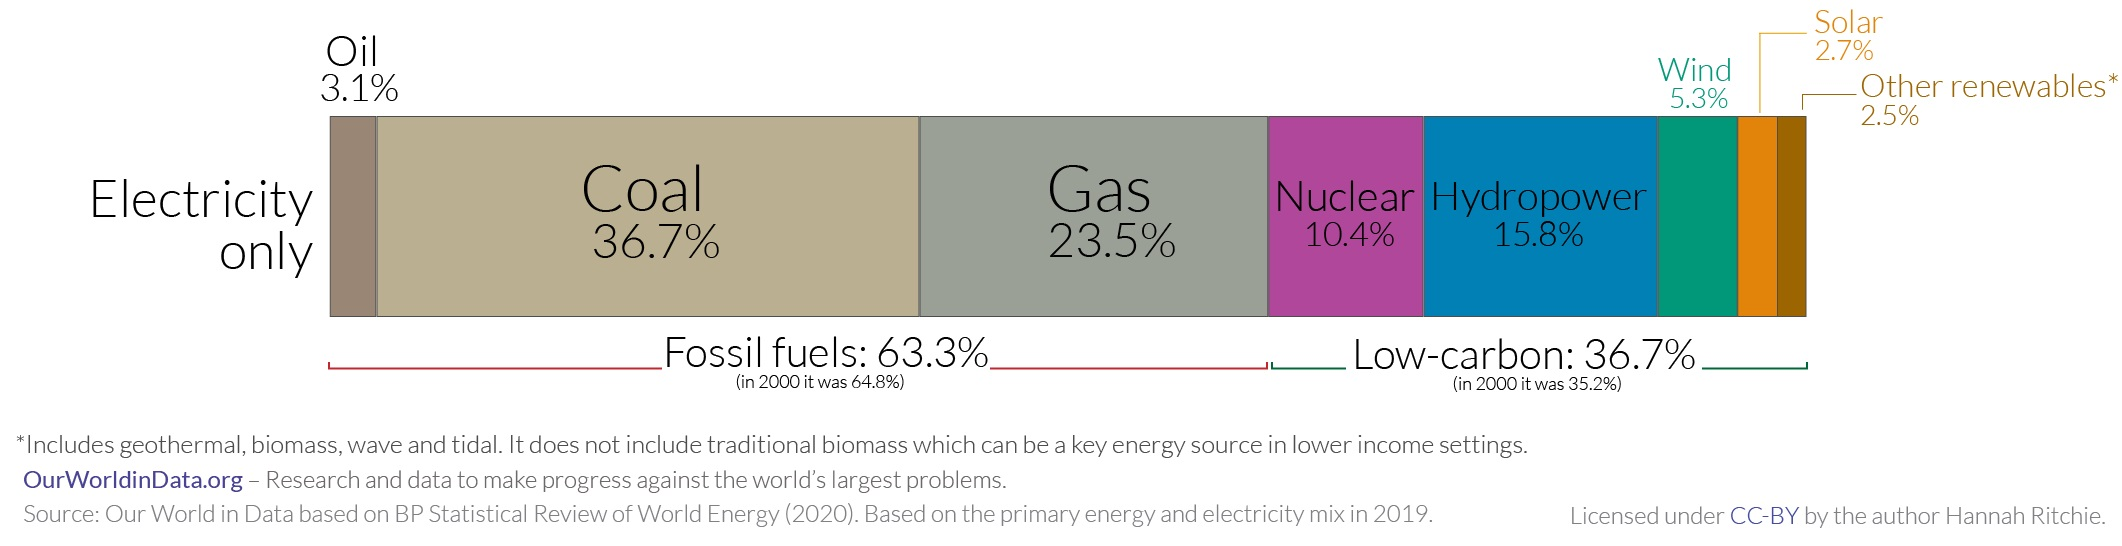
\includegraphics[width=1\textwidth]{img/Global_electricity_from_fossil_fuels.jpg}
  \caption{Global electricity production from fossil fuels\protect\footnotemark.}
  \label{fig:Global_electricity_from_fossil_fuels}
\end{figure}
\footnotetext{\url{https://ourworldindata.org/uploads/2020/08/Global-energy-vs.-electricity-breakdown-1536x812.png}}
\vspace{-10pt}

The consumption of electricity has risen due to the increased use of devices in various sectors such as home, entertainment, and more. Moreover, the number of smart devices (e;g.IoT Devices) is expected to grow more than twice by the end of this decade. By 2040, billions of IoT devices could contribute up to 14 percent of the world’s carbon emissions\footnote{\url{https://www.theguardian.com/environment/2017/dec/11/tsunami-of-data-could-consume-fifth-global-electricity-by-2025}}.

\vspace{-12pt}
\vspace{3em}
\begin{figure}[h]
  \centering
  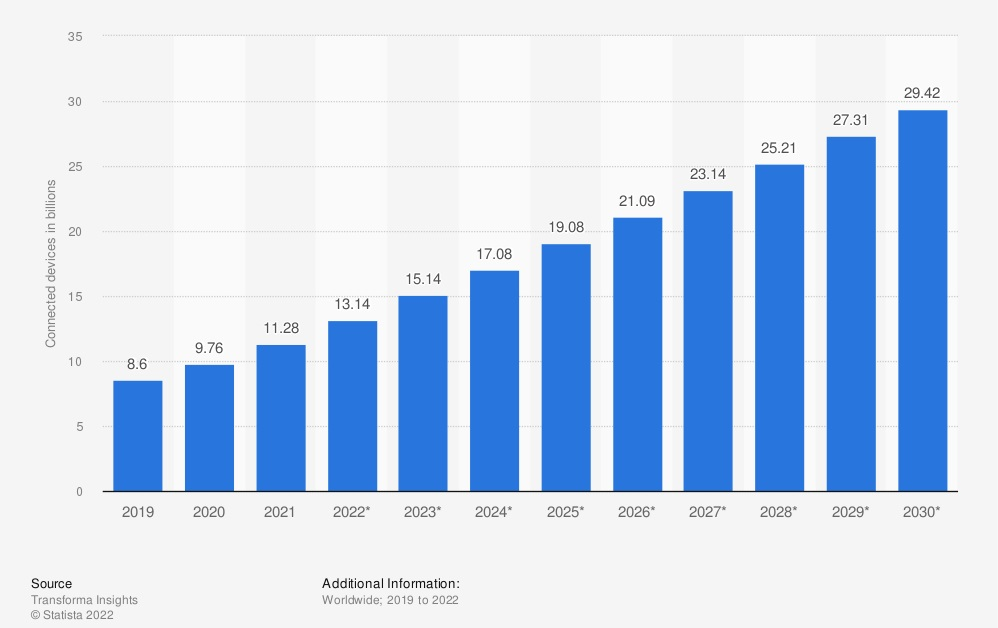
\includegraphics[width=.7\textwidth]{img/Number-of-iot-connected-devices-worldwide-2019-2021-with-forecasts-to-2030.jpg}
  \caption{Number of IOT connected devices worldwide (2019-2021) with forecasts to 2030.\protect\footnotemark}
  \label{fig:Number-of-iot-connected-devices-worldwide-2019-2021-with-forecasts-to-2030.jpg}
\end{figure}
\footnotetext{\url{https://www.statista.com/statistics/1183457/iot-connected-devices-worldwide/}}
\vspace{-15pt}

As the use of IoT devices becomes more widespread, energy consumption has become a major concern. Researchers are working on ways to make both hardware and software components of devices more energy-efficient. While software itself does not consume energy, its architecture, structure, and usage context can influence the energy consumption of hardware. By configuring software to be more energy-efficient, we can reduce energy consumption and carbon emissions, contributing to the preservation of our planet.\par


%\vspace{.5em}
%The increase in  CO\textsubscript{2} emissions leads to global warming and changes in climate and weather patterns, resulting in more floods, droughts, or intense rain, as well as more frequent and severe heat waves. The planet’s oceans and glaciers are also affected—oceans are warming and becoming more acidic, ice caps are melting, and sea level is rising. These changes present challenges to our society and our environment, including health risks from heat waves, worsening air and water quality, and the spread of certain diseases.


\vspace{.5em}
Software, gaming services on various devices, servers, networks infrastructure and data centers generate a significant amount of carbon dioxide emissions. The servers and data centers also need to use a huge amount of energy to maintain the temperature so that the machines can work more efficiently. According to a study by Abraham, every company, studio, and developer he gathered data on including Ubisoft, Nintendo, and Microsoft were all somewhere in the range of generating 1 to 5 tons of CO\textsubscript{2} per year\footnote{\url{https://www.polygon.com/features/22914488/video-games-climate-change-carbon-footprint}}. 

\begin{figure}[htbp]
  \centering
  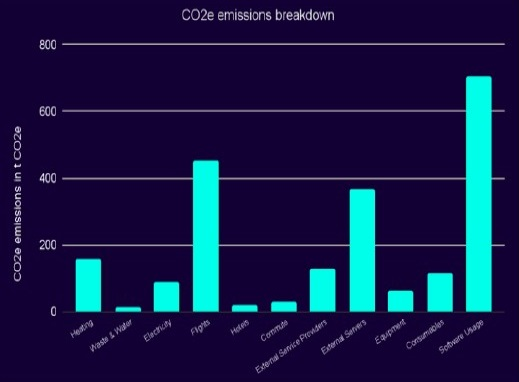
\includegraphics[width=.5\textwidth]{img/CO2_emission_each_level.jpg}
  \caption{CO\textsubscript{2}e emissions breakdown.\protect\footnotemark}
  \label{fig:CO2_emission_each_level}
\end{figure}
\footnotetext{\url{https://www.planetly.com/articles/what-tech-companies-can-do-to-reduce-and-avoid-emissions}}

\vspace{.5em}
To comprehend the energy consumption associated with software, the following examples are provided:
In 2019, researchers found that the energy used to keep the Bitcoin network running was more than the energy used by the whole country of Switzerland\footnote{\url{https://hbr.org/2020/09/how-green-is-your-software}}. Training a single neural network model today can emit as much carbon as five cars in their lifetimes\footnotemark[9]. Researchers trained an AI model to recognize different types of iris flowers. The model was 96.17\% accurate and used 964 joules of energy. To make the model 1.74\% more accurate, it needed 2,815 joules of energy. To make it just 0.08\% more accurate, it needed almost 4 times more energy than the first stage\footnotemark[9].

\vspace{.5em}
Energy consumption plays a pivotal role in contributing to global carbon dioxide emissions, making it crucial to address this issue in the context of software development. While modifying user behavior to reduce energy consumption can be challenging, there are opportunities to assist developers and other stakeholders in integrating energy efficiency considerations throughout the software development life cycle. For example: Puzzling out Software Sustainability \cite{DBLP:journals/suscom/CaleroP17}.

\vspace{.5em}
Energy efficiency is crucial in Cyber-Physical Social Systems (CPSS), which combine computing, physical processes, and social interactions. As these systems grow in complexity, they use more energy, impacting the environment. Making the software in CPSS more energy-efficient can cut down its overall energy use and reduce its carbon footprint. This not only helps the planet but also makes the system run better and be more resilient. The unique blend of tech and social elements in CPSS offers both challenges and opportunities for making it more energy-efficient. Thus, focusing on energy-smart software is key to fighting global climate change.

\vspace{-10pt}
\section{Problem Statement}
\label{sec:problem_statement}
The energy efficiency of software development is often overlooked by software developers, leading to suboptimal energy consumption in software applications. This lack of awareness and consideration for energy efficiency can be attributed to several factors:

\begin{itemize}
\vspace{-5pt}
\item Currently, there is a lack of direct energy awareness that enable software developers to measure and understand the energy consumption of their source code during the development phase. This absence hinders the ability to identify and address energy inefficiencies early on.
\vspace{-5pt}
\item Software developers generally lack sufficient knowledge and awareness about how to save energy by optimizing their source code. Without the necessary guidance and information, they may unknowingly contribute to excessive energy consumption in their software applications.
\end{itemize}

Due to its platform independence and strong security features, Java dominated the programming language landscape as the most popular choice from 2015 to 2020. Despite its decline in recent years, Java still holds a significant position as the fifth most popular programming language and continues to be extensively utilized in server environments\footnote{\url{https://insights.stackoverflow.com/survey/2020#most-popular-technologies}}. Though python is the most energy consuming Programming Language, it is also found by the researchers that Java also consumes more energy than C, C++. For example: Ranking programming languages by energy efficiency \cite{DBLP:journals/scp/PereiraCRRCFS21}. Given Java programming language's historical prominence, machine independence, security capabilities, and widespread adoption in server applications, we have selected Java as our primary focus for further research and development efforts.

\vspace{-10pt}
\section{Objectives}
\label{sec:Objectives}

In our research, we will undertake a thorough exploration of various tactics aimed at improving software energy efficiency. We will not only identify these tactics but also provide detailed insights into their implementation, highlighting practical ways to integrate them into the software development process. The main objective of this study is to explore tactics for enhancing software energy efficiency. From this objective we define 2 research questions:
\begin{itemize}
    \item RQ1: Which tactics help to improve Energy Efficiency?
    \item RQ2: How can we automatise the integration of tactics to reduce energy consumption?
    \begin{itemize}
    \item \small RQ2.1 Does the improvement of \textit{execution time} and  \textit{memory consumption} reduce energy consumption?
    \item \small RQ2.2 Could code refactoring integrate into GI? Which elements need to be extended in the Gin tool?
    \item \small RQ2.3: In which extent code refactoring genetically improve the software to reduce energy consumption?
  \end{itemize}
\end{itemize}

\vspace{-5pt}
In response to Research Question 1 (RQ1), we explore tactics for improving energy efficiency, primarily focusing on code refactoring. We explore code refactoring as our main tactic due to its significant impact on energy conservation. We will delve into various code refactoring methods, including state-of-the-art techniques. Our ultimate goal is to elucidate how this tactical approach contributes to enhancing the energy efficiency of software.\par

\vspace{.5em}
In RQ2, we focus on automating the integration of tactics to lower energy consumption. The approach involves using a genetic improvement, and as part of the research, a tool called GIN will be introduced. GIN is designed to improve existing software using search-based techniques. Three sub-questions have been identified: RQ2.1 aims to verify if improvements in response time and memory consumption(individually or together) can result in energy reduction. Experiments will be conducted using the GIN tool, with optimized versions compared to their original version using JoulerJX to assess energy impact. RQ2.2 investigates the feasibility of integrating code refactoring into Genetic Improvement (GI), identifying necessary extensions to the GIN tool. Finally, RQ2.3 explores the extent to which the integration of code refactoring can genetically enhance software to reduce energy consumption, testing its impact on energy efficiency.\par

\vspace{-10pt}
\section{Conclusion}

The efficient utilization of smart devices and the transition towards sustainable energy sources are crucial topics of global significance. It is essential for individuals and communities to remain cognizant of their electricity consumption and to promote energy efficiency. By raising awareness and making small changes in our daily lives, we can collectively contribute to reducing the strain on non-renewable resources and pave the way for a greener, more sustainable future.

\vspace{.5em}
The research comprised several distinct chapters. In the first chapter, the motivation behind the study, the objectives to be achieved, and the problem statement were discussed. In the second chapter, we delved into tactics for enhancing software energy efficiency, analyzed their respective benefits and limitations, and identified a tactic. Additionally, we emphasized the importance of energy consumption monitoring and selected \textit{JoularJX} as our primary tool for monitoring energy consumption in Java-based applications. The third chapter provided an in-depth literature review focusing on the themes of code refactoring and genetic improvement in software. Chapter four detailed a preliminary study aimed at understanding software energy consumption using the \textit{JoularJX} tool, illustrating its installation process and the initial experiments that were conducted using this tool. In Chapter five, we presented the results of our experiments, compared the energy consumption of the original and optimized programs using the \textit{Gin} tool, and discussed the implications for software energy efficiency. The sixth chapter was for the conclusion and discussions on future work.



\chapter{Background}
The initial motivation and primary focus of this research work is to explore tactics for enhancing software energy efficiency. With this in mind, we  answer the first research question:

\vspace{1em}
\textbf{RQ1}: Which tactics help to improve Energy Efficiency?

\vspace{1em}
Enhancing software energy efficiency is an important goal in the development of modern software systems. Several tactics can be used to achieve this goal, including Architectural Tactics, Design Patterns, and Code Refactoring. 

\begin{itemize}
    \item \textbf{Architectural Tactics}:These tactics focus on adapting the software architecture for energy efficiency. For example, \cite{DBLP:conf/hicss/ParadisKT21} provide a basis for reasoning about design decisions for energy efficiency by deriving a set of reusable architectural tactics derived from the research literature, via a taxonomic literature review. Researchers used an open-search and snowballing methodology to obtain primary studies and then used thematic coding to identify commonalities among the design strategies described. The result of this process is a taxonomy of 10 architectural tactics for energy efficiency, which provide a rational basis for architectural design and analysis for energy efficiency. These tactics are grouped into three broad categories: Resource Monitoring, Resource Allocation, and Resource Adaptation. These categories serve as a high-level checklist for a software architect or a reviewer, and the true design thinking goes into how those categories are refined into specific tactics and how those tactics are in turn translated into code, patterns, and components.
    \item \textbf{Design Patterns}:These are reusable solutions to common problems in software design that can be used to improve energy efficiency. For example, \cite{DBLP:conf/icse/NoureddineR15} presents a vision to automatically detect and transform design patterns during compilation for better energy efficiency without impacting existing coding practices. The authors propose compiler transformations for two design patterns, Observer and Decorator, and perform an initial evaluation of their energy efficiency. 
    \item \textbf{Code Refactoring}:This is the process of restructuring existing code without changing its external behavior(i.e. functionalities) to improve its readability and maintainability. Refactoring techniques aim to reduce the energy consumption of the software. \cite{csanlialp2022energy} examines the effect of code refactoring techniques(e.g. Encapsulate field, Inline temp, Simplify nested loop) on energy consumption. A total of 25 different source codes of applications programmed in the C\# and Java languages are selected for the study, and combinations obtained from refactoring techniques are applied to these source codes. The results show that the combinations significantly improve the software’s energy efficiency.
\end{itemize}

We are providing a comparative analysis between the mentioned tactics. This is not an exhaustive study but it provides a general overview of advantages and limitations of these techniques:
\vspace{1em}
{\footnotesize
\begin{longtable}{|p{1.6cm}|p{3.5cm}|p{3cm}|p{3.5cm}|p{3.5cm}|}
  \hline
  \textbf{Tactic} & \textbf{Purpose} & \textbf{Advantages} & \textbf{Limitations} & \textbf{Example of reference} \\
  \hline
  Architectural Tactics &
 provide a basis for reasoning about design decisions for energy efficiency in software architectures. The paper derives a set of reusable architectural tactics for energy efficiency from the research literature, via a taxonomic literature review. Researchers used an open-search and snowballing methodology to obtain primary studies, and then used thematic coding to identify commonalities among the design strategies described. The result of this process is a taxonomy of 10 architectural tactics for energy efficiency. These tactics provide a rational basis for architectural design and analysis for energy efficiency. & 
 Provide a rational basis for architectural design and analysis for energy efficiency. By using mentioned tactics, software architects can make informed decisions about how to design their systems to be more energy-efficient. This can help reduce the environmental impact of software, as well as improve the battery life of mobile and IoT devices. Additionally, by using an architectural approach to energy efficiency, software engineers can better manage complex system-wide properties, which can be difficult to address through coding alone. & 
 Need for a comprehensive framework that can enumerate relevant contextual factors and assist in reasoning about the consequences of design decisions on energy efficiency and other quality attributes. The absence of such a framework makes it difficult for architects and developers to make informed decisions. &
 ~\cite{DBLP:conf/hicss/ParadisKT21} \\
 \hline
 Design Patterns & 
 Explore the ways to improve the energy efficiency of software design patterns while retaining their essential benefits, such as improved code readability and maintainability. In this study researchers propose compiler transformations for two design patterns, Observer and Decorator, and perform an initial evaluation of their energy efficiency. Their vision is to automatically detect and transform design patterns during compilation for better energy efficiency without impacting existing coding practices & 
 Several advantages of the proposed approach to improving the energy efficiency of software design patterns include: Developer coding practices remain unaffected. Benefits of using design patterns are retained. Energy consumption of software is reduced. & 
 The study focuses on only two patterns (Decorator and Observer), limiting generalization.The empirical evaluation is based on a small set of programs, potentially limiting applicability.Transformations for energy optimization are applied manually, needing automation for scalability.& 
 ~\cite{DBLP:conf/icse/NoureddineR15}\\
 \hline
 Code Refactoring & 
 Restructure existing code without changing its external behavior to enhance reusability and maintainability of software components through improving nonfunctional attributes of the software.& 
 Improve code readability, reduce complexity, and make the code more efficient, maintainable, and easier to understand.  Some refactoring techniques aim to reduce the energy consumption of the software, which can improve its energy efficiency.Refactoring transforms a mess into clean and simple code. & 
 Code refactoring for energy efficiency can be a complex and time-consuming process that requires a deep understanding of the software and its energy consumption characteristics. & 
 ~\cite{csanlialp2022energy}
 and
 ~\cite{DBLP:journals/cluster/KimHYL18}\\
 \hline
\caption{Comparison between the mentioned tactics}
\label{tab:Comparison between all mentioned tactics}
\end{longtable}
}

Unlike other tactics, code refactoring suits various types of software. By applying code refactoring, we can improve code simplicity, readability, reduce complexity, and enhance code efficiency, leading to improved energy efficiency. This answers our \textbf{RQ1}. Further exploration of code refactoring for energy-efficient software will be discussed in chapter \ref{ch:literature_review}.




\vspace{.5em}
Monitoring energy use is a crucial prerequisite before embarking on our main experiments, as accurately measuring energy consumption is paramount. Without understanding the energy usage of programs, progress to our main experiments becomes uncertain. It is essential to determine which tool will be the most efficient for measuring energy consumption. To achieve this, we explore various tools, each with its advantages and drawbacks. In this subsequent section, we will discuss the advantages and drawbacks of various tools.

\section{Energy Consumption Profiling Tools}

Measuring energy consumption is challenging because there's no straightforward way for directly measuring energy usage. To overcome this, we rely on external tools to measure energy. 
Energy consumption measuring tools can be categorized mainly in two categories:
\begin{itemize}
    \item \textbf{Hardware Tools}: Wattmetter ~\cite{bekaroo2014power}
    \item \textbf{Software Tools}:
    \begin{itemize}
    \item {Power Joular ~\cite{DBLP:conf/intenv/Noureddine22}}
    \item {JoularJX ~\cite{DBLP:conf/intenv/Noureddine22}}
    \item {Likwid Powermeter\footnote{\url{https://github.com/RRZE-HPC/likwid/wiki/Likwid-Powermeter}}~\cite{DBLP:journals/corr/abs-1004-4431}}
    \end{itemize}
\end{itemize}

As our aim is to determine which tool will be the most efficient for measuring the energy consumption of a software program, we will mainly focus on software tools. Now, we will provide a description of all the aforementioned software tools.\par \vspace{1em}

\textbf{PowerJoular}: PowerJoular is a command line software to monitor, in real time, the power consumption of software and hardware components.\\

\textbf{Advantages}:
\begin{itemize}
    \renewcommand\labelitemi{}
    \item It can measure the CPU, GPU and memory consumption. It writes the power consumption in a CSV file.
\end{itemize}

\textbf{Disadvantages}:
\begin{itemize}
    \renewcommand\labelitemi{}
    \item Power Joular can only measure the power consumption of Intel RAPL (CPU) and NVIDIA SMI (GPU).
\end{itemize}

\textbf{JoularJX}: JoularJX is a Java-based agent for software power monitoring at the source code level\\

\textbf{Advantages}:
\begin{itemize}
    \renewcommand\labelitemi{}
    \item JoularJX works as a java agent. It hooks to the JVM (Java Virtual Machine) to monitor power consumption. It can get power and energy consumption at the method level.
\end{itemize}

\textbf{Disadvantages}:
\begin{itemize}
    \renewcommand\labelitemi{}
    \item JoularJX can only measure the energy and power consumption for the Java source codes and applications.
\end{itemize}

\textbf{Likwid Powermeter}:Likwid Powermeter is a
tool for accessing RAPL(Running Average Power Limit) counters on Intel processors, which allows you to query the energy consumed within a package for a given time period and computes the resulting power consumption.\\

\textbf{Advantages}:
\begin{itemize}
    \renewcommand\labelitemi{}
    \item It can monitor the energy consumption by the core of the CPU of the machine, provide the result by measuring the energy consumption by each processor.
\end{itemize}

\textbf{Disadvantages}:
\begin{itemize}
    \renewcommand\labelitemi{}
    \item It can not able to monitor the energy consumption methodwise. Provide processorwise results (at the level of CPU cores), sometimes results can vary as other processes may run on the same core with the test process.
\end{itemize}

\vspace{.5em}
From the mentioned energy consumption monitoring software tools, we chose JoularJX to run our experiments and measure energy and power consumption. The key reason for selecting JoularJX is that it allows real-time monitoring at the source code level. It functions as a Java agent, providing accurate power and energy readings on both GNU/Linux and Windows platforms. This makes it a suitable tool for monitoring the energy consumption of Java-based software or Java-based programs. As mentioned in Chapter \ref{ch:Introduction}, Section \ref{sec:problem_statement}, our primary focus is on Java programs or Java-based software for making energy-efficient, which makes JoularJX the appropriate choice for our requirements.


\section{Conclusion}
 In our quest to enhance software energy efficiency, we explored various tactics, such as Architectural Tactics, Design Patterns, and Code Refactoring. Through comparative analysis, we discerned the benefits and limitations of each tactic, with code refactoring proving to be versatile across diverse software types.This provided the answer to our first research question \textbf{RQ1}. Monitoring energy consumption is pivotal to this research. Among the software tools considered for profiling energy consumption, JoularJX emerged as the most appropriate for our Java-based software focus. 

\chapter{Literature Review}
%: Code Refactoring, Genetic Improvement and Gin Tool
\label{ch:literature_review}
%\section{Introduction}
Conducting a literature review is an essential step in any research project. In this section, we reviewed research papers related to the internship's topics, including code refactoring for improving software energy efficiency and genetic improvement for getting better versions of software. Through this review, we assessed the strengths and limitations of the existing research. 

\vspace{.5em}
The insights gained from this review were in identifying potential code refactoring techniques for improving software energy efficiency, this answering RQ2.

\section{Code Refactoring for Software Energy Efficiency}
%In this section, we will review the existing research on code refactoring, exploring its significance and advantages. Additionally, we will investigate various available code refactoring techniques, conducting a comparative analysis to identify the most suitable code refactoring techniques. Subsequently, we will select the suitable code refactoring techniques for integration into the gin tool, based on the findings of our comparison. 

%\subsection{Code Refactoring}

Code refactoring is the process of restructuring existing computer code without changing its external behavior to enhance reusability and maintainability of software.
%components through improving nonfunctional attributes of the software ~\cite{DBLP:journals/cluster/KimHYL18}. It is a way to improve the code quality and maintainability\footnote{\url{https://www.c-sharpcorner.com/article/pros-and-cons-of-code-refactoring/}}. 
The benefits of code refactoring include removing bad smells, reducing code size, improving readability, and making it easier to enhance and maintain in the future. However,
the main limitations of applying code refactoring is that could be time expensive and error-prone. So, its automatising is crucial for supporting developers and architects. 
%there are also limitations to code refactoring. For example, it can be time consuming and 
%expensive and risky in the view of management, may introduce bugs, and can be difficult to do if the code is already a big mess. Additionally, refactoring should not be done if a deadline is near or if the cost of refactoring is higher than rewriting the code from scratch\footnotemark[1]. 

\vspace{.5em}
In the context of energy efficiency, code refactoring can be used to improve the energy consumption of software by making changes to the source code that reduce its energy usage. Several studies have investigated the impact of code refactoring on energy consumption (see Table~\ref{tab:comparison} that presents three main studies in this domain). 

\cite{DBLP:conf/esem/SahinPC14} presented an empirical study to investigate the energy impacts of 197 applications using 6 commonly-used code refactoring methods, for instance \texttt{Convert Local Variable to Field} (see Row 1 in Table~\ref{tab:comparison}). The results show that code refactoring methods can not only impact energy usage but can also increase and decrease the amount of energy used by an application. 

%Another study~\cite{DBLP:conf/icsoft/OurnaniRRP21a} found that developers can optimize the power consumption of software by improving their source code implementations. 
\cite{DBLP:journals/tse/MoralesSKCA18} proposed a code smell or anti-pattern correction approach called EARMO. EARMO is a multi-objective search based technique that improves energy efficiency and the quality of code by using code refactoring. In this study, the researchers analyzed the impact of eight types of anti-patterns, for instance \texttt{Move Method} that refactors the \texttt{Bob (God class)} code smell (see Row 2 in Table~\ref{tab:comparison}).
%on a testbed of 20 android apps extracted from F-Droid and evaluated EARMO using three multi-objective search-based algorithms. 
%The results showed that 
EARMO is able to
%can generate refactoring recommendations in less than a minute and 
remove a median of 84\% of code smells or anti-patterns. Moreover, EARMO extended the battery life of a mobile phone by up to 29 minutes. 
%when running a refactored multimedia app with default settings (no Wi-Fi, no location services, and minimum screen brightness) in isolation. 
%A qualitative study was also conducted with developers of the studied apps to assess the refactoring recommendations made by EARMO. 
An experiment with developer showed that EARMO suggest 68\% of code refactoring  are relevant for improving the quality of code and energy efficiency. 
%suggested by EARMO to be very relevant. 
%Additionally, code smells, which are symptoms of poor design or implementation choices, have been found to impact energy consumption. 

\cite{DBLP:journals/infsof/PalombaNPZL19} founded that code refactoring for android applications, for instance refactoring the \texttt{Data Transmission Without Compression} code smell (see Row 3 in Table~\ref{tab:comparison}), is able to reduced energy consumption by up to 10.8\%. Moreover, four code smells increase method energy consumption by up to 87 times.


\begin{table}[!h]
\centering
\scalebox{0.8}{
\begin{tabular}{|p{3.5cm}|p{6.5cm}|p{5cm}|p{2cm}|p{2cm}|}

\hline
\textbf{Reference} & \textbf{Code refactoring} & \textbf{Experiment / Bench-marking} & \textbf{Tool for EC} & \textbf{Results}  \\

\hline
\cite{DBLP:conf/esem/SahinPC14} & 
\textbf{Code refactoring (6)}: Convert Local Variable to Field,
Extract Local Variable,
Extract Method,
Introduce Indirection, 
Inline Method
Introduce Parameter Object & 
9 Java Applications (ex. cMath, cCollections, ..) & 
Low Power Energy Aware Process (LEAP) & 
-7.50\% to 4.54\%  \\
\hline

\cite{DBLP:journals/tse/MoralesSKCA18} & 
\textbf{Android code smells (3)}: Binding resources too early class, Private getter and setters, HashMap usage. \textbf{OO code smells (5)}: Lazy class, Blob (God class), Long-parameter list, Refused bequest, Speculative Generality & 
\textbf{Phase 1:} Empirical Study to understand in which extent 8 code refactorings help to save energy. 
\textbf{Phase 2:} EARMO is developped to select optimal series of code refactoring.  The energy consumed by the version of code is inferred from Phase 1. & 
Not reported. &
EARMO is able to save 29 minutes of battery.
\\
\hline

\cite{DBLP:journals/infsof/PalombaNPZL19} & 
\textbf{Android-specific code smells (9)}: Data Transmission Without Compression, Durable Wakelock, Inefficient Data Structure, Inefficient SQL Query, Inefficient Data Format And Parser, Internal Setter, Leaking Thread,  Member-Ignoring Method, Slow Loop & 
60 Android Java apps (categories ex. games, productivity, social, etc) & 
PETRA (Power Estimation Tool for Android) & 
Four code smell types increase method energy consumption by up to 87 times.
\\
\hline
\end{tabular}
}
\caption{Comparison of approaches}
\label{tab:comparison}
\end{table}

According to the information mentioned above, it can be concluded that code refactoring can have a positive impact on energy efficiency by reducing the energy consumption of software. However, the benefits and limitations of code refactoring for energy efficiency may vary depending on the specific context and implementation.

%\subsection{Types of Code Refactoring Techniques and Comparison between mentioned Code Refactoring Techniques}

\vspace{.5em}
In Table \ref{tab:Types_Code_Refactoring_Techniques}, we present the 
%different types of 
code refactoring techniques studied in the previous works. We introduce them because the authors of these works provided individual information about their positive impact in energy efficiency. So, it provides us more insights about their usefulness in software energy efficiency.
%and compare them based on energy consumption impact 

{\footnotesize
\begin{longtable}{|c|p{2cm}|p{4.3cm}|p{8cm}|}
%\begin{table}[ht!]
%\caption{Types of Code Refactoring Techniques}
%\label{tab:Types_Code_Refactoring_Techniques}
%\scalebox{0.8}{
%\begin{tabular}{|c|p{2cm}|p{4cm}|p{13cm}|}

  \hline
\textbf{Ref.} &  \textbf{Code Refactoring Technique} & \textbf{Purpose} & \textbf{Energy Consumption Impact}\\
  
  \hline
\multirow{6}{*}{\rotatebox[origin=rc]{90}{\cite{DBLP:conf/esem/SahinPC14}}} &
  Convert Local Variable to Field
  %~\cite{DBLP:conf/esem/SahinPC14} 
  & 
  Turns a local variable into a field. &
  This refactoring had a statistically significant difference in energy usage in some cases for JVM. This means that in some cases, applying this refactoring resulted in a noticeable change in the amount of energy used by the program. In most cases, applying this refactoring resulted in an decrease in the amount of energy used by the program.  \\
  
 \cline{2-4}
 & Extract Local Variable
 %~\cite{DBLP:conf/esem/SahinPC14} 
 & 
 Creates a new variable assigned to the selected expression and replaces the selection with a reference to the new variable. &
 It had the least impact on energy usage, with only a few cases showing a significant difference. This means that in most cases, applying this refactoring did not result in a noticeable change in the amount of energy used by the program. In some cases, for JVM 6, the amount of energy used by the program decreases\\
  
 \cline{2-4}
 & Extract Method 
  %~\cite{DBLP:conf/esem/SahinPC14}
  & 
  Creates a new method containing the selected statement or expression and replaces the selection with a reference to the new method. &
  This refactoring increased energy usage 8 times and decreased energy usage 2 times on JVM6. This means that in most cases, applying this refactoring resulted in an increase in the amount of energy used by the program. However, in a few cases, there was a decrease in energy usage after applying this refactoring.\\
  
 \cline{2-4}
 & Inline Method 
  %~\cite{DBLP:conf/esem/SahinPC14} 
  & 
  Copies the body of a called method into the body of a caller method. &
  It had varying impacts on energy usage across different applications and platforms. This means that the impact of this refactoring on energy usage is not consistent and can vary depending on the specific application and platform. In some cases, it may reduce energy usage, while in others it may increase it. \\
  
 \cline{2-4}
 & Introduce Indirection
 %~\cite{DBLP:conf/esem/SahinPC14} 
 & 
 Creates a static method to indirectly delegate to the selected method. &
 This refactoring had both positive and negative impacts on energy usage. This means that the impact of this refactoring on energy usage is not consistent and can vary depending on the specific case. In most cases, applying this refactoring resulted in an increase in the amount of energy used by the program. However, in a few cases, there was a decrease in energy usage after applying this refactoring. \\
  
 \cline{2-4}
 & Introduce Parameter Object
 %~\cite{DBLP:conf/esem/SahinPC14} 
 & 
 Replaces a set of parameters with a new class and updates all callers to pass an instance of the new class as the value to the introduced parameter. &
 It had a significant impact on energy usage. This means that in most cases, applying this refactoring resulted in a decrease in the amount of energy used by the program. \\
 
  \hline 
\multirow{1}{*}{\rotatebox[origin=rc]{90}{\cite{DBLP:conf/seke/ParkHL14}}} & Encapsulate Field  & 
  Set access permissions of a variable by creating getters and setters for the selected field, allowing the field to be accessed and modified only through these methods. This provides better control over the field and can improve the maintainability of the code. &
  This technique can have an impact on energy efficiency, especially when combined with other code refactoring techniques. These combinations can provide significant improvements in energy efficiency. \\
  
 \hline 
\multirow{1}{*}{\rotatebox[origin=rc]{90}{\cite{barack2018effectiveness}}} & Inline Temp
 & 
 Replace all references to a temporary variable with the expression that was assigned to it. This can improve code readability and reduce the number of variables in the code. \vspace{1.5cm} &
 Eliminating temporary variables speeds up the fetching of redundant temporary variables from both the main and cache memories. This approach improves performance and maintains the same level of energy efficiency, which is considered a positive improvement. \\
  
 \hline
\multirow{1}{*}{\rotatebox[origin=rc]{90}{\cite{DBLP:journals/tse/MoralesSKCA18}}}  & Move Method for refactoring the Blob (God class) code smell
   & 
  Improve the organization of code by moving a method to a more appropriate class or object. \vspace{2cm} &
  Can reduce energy consumption by improving the efficiency of the code. \\
  
 \hline 
\multirow{1}{*}{\rotatebox[origin=rc]{90}{\cite{kim2018code}}} & Simplify Nested Loop
  & 
 Reduce the dimensions of multi-dimensional loops. \vspace{2cm} &
 Dimension reduction of multi-dimensional loops helps to reduce energy consumption and make the code more readable and energy-efficient. \\
  

 \hline
\caption{Types of Code Refactoring Techniques}
\label{tab:Types_Code_Refactoring_Techniques}
\end{longtable}
}
%\end{tabular}}
%\end{table}

%\subsection{Analysis and Selection of Code Refactoring Methods for Integration into the Gin Tool}

%The analysis of various code refactoring techniques, as presented in the table \ref{tab:Types of Code Refactoring Techniques}, reveals distinct patterns in their impact on energy consumption. Several techniques,  including 
From Table~\ref{tab:comparison}, we can observe that \texttt{Convert Local Variable to Field}, \texttt{Introduce Parameter Object}, \texttt{Inline Temp}, \texttt{Move Method}, \texttt{Simplify Nested Loop} and \texttt{Encapsulate Field}, consistently show positive results in reducing energy consumption across different scenarios. 
%
%Moreover, the combined application of \texttt{Inline Temp}, \texttt{Simplify Nested Loop}, and \texttt{Encapsulate Field} code refactoring techniques proves to be particularly effective in enhancing energy efficiency ~\cite{csanlialp2022energy}.
%
%\vspace{.5em}
Conversely, \texttt{Extract Local Variable}, \texttt{Extract Method}, \texttt{Inline Method}, and \texttt{Introduce Indirection} exhibit varying effects on energy consumption depending on the specific context. Hence, it is essential to apply these techniques with caution and consider the unique circumstances of each code-base.

\vspace{.5em}
For integrating code refactoring techniques into the
a genetic improvement method %Gin Tool 
for improving software energy efficiency, we can consider 
%, our top priority would be to incorporate 
the \texttt{Convert Local Variable to Field} and \texttt{Introduce Parameter Object} code refactoring techniques because they consistently yield energy reductions for Java programming. Moreover, the \texttt{Move Method} code refactoring technique
%, primarily used for Mobile Apps, 
can be considered for Java applications to enhance energy efficiency. Finally, the integration of \texttt{Inline Temp}, \texttt{Simplify Nested Loop}, and \texttt{Encapsulate Field} code refactoring techniques would be valuable, as they have demonstrated consistent energy consumption improvements in various cases. 
%By making these selective and informed choices, we aim to enhance the Gin Tool's capabilities and provide developers with effective means to optimize energy consumption in their codebases.


\section{Genetic Improvement (GI)}
%In this section, we will discuss the Genetic Improvement (GI) and Gin Tool. We will explore the strengths and limitations of existing research on genetic improvement and gin tool. We will also justify our selection of the gin tool for obtaining an improved version of the program based on the best patch for lower fitness function and identify specific components of the gin tool that need extension to integrate the selected code refactoring techniques, which aligns with Research Question \textbf{RQ2.2}. 

%\subsection{Genetic Improvement (GI)}

Genetic Improvement (GI) is a field of research that uses automated search to find improved versions of existing software. It can improve both functional properties of software, such as bug repair, and non-functional properties, such as execution time, energy consumption, or source code size~\cite{DBLP:journals/tec/PetkeHHLWW18,DBLP:conf/gecco/ZuoBP22}. 

\vspace{.5em}
Genetic Improvement (GI) is an optimization technique inspired by natural evolution to enhance software. The process starts with an initialization phase where a set of software solutions (individuals) is created. Each solution's efficacy is gauged using a fitness function. If the stopping criteria are not met, which can be a specific fitness level or a number of iterations, the solutions undergo mutations to introduce variability. This altered set is then re-evaluated. The cycle of evaluation, checking stopping criteria, and mutation continues until the stopping criteria are met, at which point the best solution is identified as optimal. Throughout this process, GI aims to find a satisfactory software version based on predefined metrics, though a global optimum is not always guaranteed.

\begin{figure}[h]
  \centering
  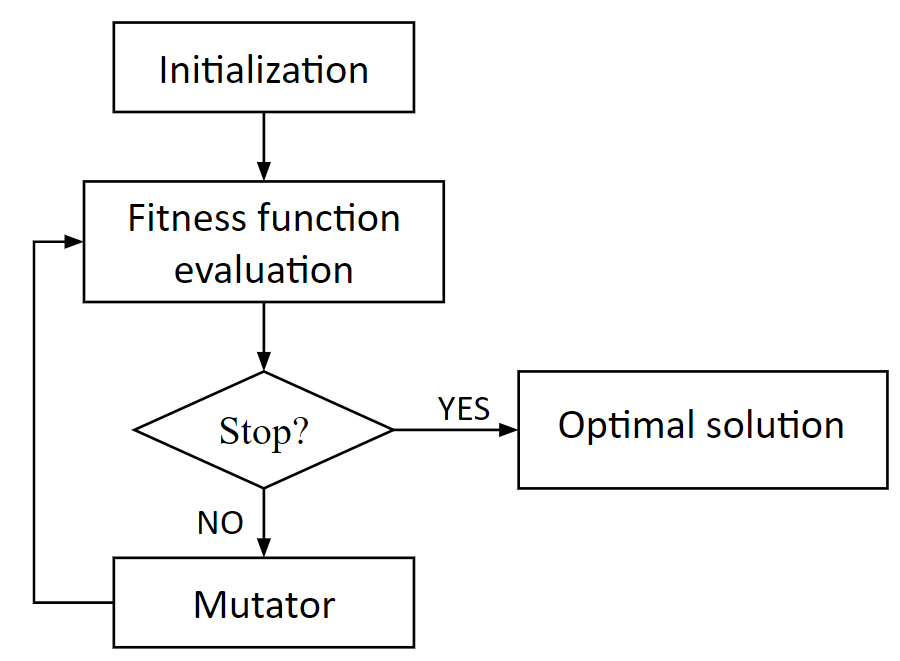
\includegraphics[width=.5\textwidth]{img/Genetic_Improvement_.png}
  \caption{Overall process of genetic improvement}
  \label{fig:Genetic_improvement_process}
\end{figure}


%Researchers have already shown that GI can improve human-written code, ranging from program repair to optimizing run-time, from reducing energy consumption to the transplantation of new functionality~\cite{DBLP:conf/gecco/BrownleePABWW19}.

\vspace{.5em}

%Numerous research studies have been conducted in the Genetic improvement domain.
%
%In Table \ref{tab:Genetic Improvement Research Papers Summary} below, we present a compilation of relevant research works that are well-suited for supporting and enhancing our own research exploration. The table includes key information about each work, such as title, author name, and key findings.

\cite{DBLP:journals/tec/PetkeHHLWW18} presents a comprehensive survey of  
%the nascent field of research 
research studies on GI that were published between 1995 and 2015.
%,  with a focus on the core papers in the area published between 1995 and 2015. 
Authors identified 
%core publications including empirical studies, 
that 96\% of these studies use evolutionary algorithms (in particular genetic programming). Moreover, GI has resulted in performance improvements for a diverse set of properties such as execution time and memory consumption, as well as results for fixing and extending existing system functionality. However, only three studies focused on reducing energy consumption were mentioned in this survey. These studies are described as follows:

\begin{itemize}
    \item \cite{DBLP:conf/gecco/BrucePH15} applied GI to the \textit{MiniSAT Boolean Satisfiability} solver when specializing for three downstream applications and found that GI can successfully be used to reduce energy consumption by up to 25\%.
    
    \item \cite{DBLP:conf/gecco/MrazekVS15} presented a method based on \textit{Cartesian genetic programming} that is evaluated in the task of approximation of 9-input and 25-input median function. Resulting approximations shown a significant improvement in the execution time and power consumption with respect to the accurate median function while the observed errors are moderate.
    
    \item \cite{DBLP:conf/ssbse/BurlesBBKSV15} used a \textit{metaheuristic search} to improve Google’s Guava library by finding a semantically equivalent version of \texttt{com.google.common.collect.ImmutableMultimap} with reduced energy consumption. Semantics-preserving transformations were found in the source code using the principle of subtype polymorphism. A new tool, \texttt{Opacitor}, was introduced to deterministically measure energy consumption and it was found that a statistically significant reduction to Guava’s energy consumption is possible. 
\end{itemize}


%{\footnotesize
%\begin{longtable}{|p{4.3cm}|p{3.2cm}|p{8.5cm}|}

%  \hline
%  \textbf{Title} & \textbf{Author Name} & \textbf{Key Findings}\\
  
%  \hline
%  Genetic Improvement of Software: A Comprehensive Survey ~\cite{DBLP:journals/tec/PetkeHHLWW18} & 
%  Justyna Petke, Saemundur O. Haraldsson, Mark Harman, William B. Langdon, David R. White, and John R. &
%  Present a comprehensive survey of the nascent field of research on Genetic Improvement (GI) with a focus on the core papers in the area published between 1995 and 2015. Authors identified core publications including empirical studies, 96\% of which use evolutionary algorithms (genetic programming in particular). GI has resulted in performance improvements for a diverse set of properties such as execution time, energy and memory consumption, as well as results for fixing and extending existing system functionality.\\
   
%  \hline
%   Gin: Genetic Improvement Research Made Easy ~\cite{DBLP:conf/gecco/BrownleePABWW19} & 
%   Alexander E.I. Brownlee, Justyna Petke, Brad Alexander, Earl T. Barr, Markus Wagner, and David R. &
%   Introduced an extensible and modifiable GIN toolbox for GI experimentation, with a novel combination of features. Instantiated in Java and targeting the Java ecosystem, Gin automatically transforms, builds, and tests Java projects and supports automated test generation and source code profiling. The study showed through examples and a case study how Gin facilitates experimentation and can speed up innovation in GI.\\
   
%   \hline
%   Evaluation of Genetic Improvement Tools for Improvement of Non-functional Properties of Software ~\cite{DBLP:conf/gecco/ZuoBP22} &
%   Shengjie Zuo, Aymeric Blot, Justyna Petke &
%   The study conducted a literature review of available GI tools and ran multiple experiments on the found open-source tools to examine their usability. It applied a cross-testing strategy to check whether the available tools can work on different programs. Overall, the study found 63 GI papers that use a GI tool to improve non-functional properties of software, out of which 31 are accompanied by open-source code. The study was able to successfully run eight GI tools and found that ultimately only two, Gin, and PyGGI, can be readily applied to new general software.\\
   
%   \hline
%   Multi-Objective Genetic Improvement: A Case Study with EvoSuite ~\cite{DBLP:conf/ssbse/CallanP22} & 
%   James Callan and Justyna Petke &
%   Present an extension of an existing generalist, open-source genetic improvement tool, Gin, with a multi-objective search strategy, NSGA-II. The implementation was conducted on a mature, large software, EvoSuite, a tool for automatic test case generation for Java. The multi-objective extension of Gin was utilized to improve both the execution time and memory usage of EvoSuite. The study found improvements in the execution time of up to 77.8\% and improvements in memory usage of up to 9.2\% on the mentioned test set.\\
   
%   \hline
%   Reducing Energy Consumption Using Genetic Improvement ~\cite{DBLP:conf/gecco/BrucePH15} &
%   Bobby R. Bruce,\kern0.2em Justyna Petke and Mark Harman &
%   Applied GI to the MiniSAT Boolean satisfiability solver when specializing for three downstream applications and found that GI can successfully be used to reduce energy consumption by up to 25\%.\\
   
%   \hline
%    Evolutionary Approximation of Software for Embedded Systems: Median Function ~\cite{DBLP:conf/gecco/MrazekVS15} &
%    Vojtech Mrazek, Zdenek Vasicek, Lukas Sekanina &
%    The study presented a method based on Cartesian genetic programming that is evaluated in the task of approximation of 9-input and 25-input median function. Resulting approximations shown a significant improvement in the execution time and power consumption with respect to the accurate median function while the observed errors are moderate. \\
   
%   \hline
%    Object-Oriented Genetic Improvement for Improved Energy Consumption in Google Guav ~\cite{DBLP:conf/ssbse/BurlesBBKSV15} &
%    Nathan Burles, Edward Bowles, Alexander E. I. Brownlee, Zoltan A. Kocsis, Jerry Swan and Nadarajen Veerapen &
%    In this study, the authors used a metaheuristic search to improve Google’s Guava library by finding a semantically equivalent version of com.google.common.collect.ImmutableMultimap with reduced energy consumption. Semantics-preserving transformations were found in the source code using the principle of subtype polymorphism. A new tool, Opacitor, was introduced to deterministically measure energy consumption and it was found that a statistically significant reduction to Guava’s energy consumption is possible. \\
%   \hline
%\caption{Genetic Improvement Research Papers Summary}
%\label{tab:Genetic Improvement Research Papers Summary}
%\end{longtable}
%}

After a thorough analysis of existing research work on GI, it becomes evident that GI is a powerful technique that can be used to automatically find improved versions of existing software with respect to various non-functional properties such as execution time, energy consumption, memory usage, etc. Several tools have been developed to facilitate experimentation with GI, including \textit{Gin} and \textit{PyGGI}. These tools have been successfully applied to various software systems, resulting in significant improvements in performance. 

%In the subsequent subsection \ref{sub:Justify the selection of the Gin Tool for the improvement of non-functional properties of software}, we will discuss about the selection of Gin tool and justify why this tool will be suitable for our work. 

%\subsection{Justify the selection of the Gin Tool for the improvement of non-functional properties of software}

%\label{sub:Justify the selection of the Gin Tool for the improvement of non-functional properties of software}
\vspace{.5em}
\cite{DBLP:conf/gecco/ZuoBP22} conducted a literature review of available GI tools and ran multiple experiments on the found open-source tools to examine their usability. It applied a cross-testing strategy to check whether the available tools can work on different programs. The study found 63 GI papers that introduce a GI tool to improve non-functional properties of software, out of which 31 are accompanied by open-source code. From these tools, the study was able to successfully run 8 GI tools.
%and found that ultimately only two, Gin, and PyGGI, can be readily applied to new general software.
%According to~\cite{DBLP:conf/gecco/ZuoBP22}, the authors found 63 papers that introduced a GI tool to improve non-functional properties of software, of which 31 introduced open-source codes,
%The usability study of this research exposed 11 different general GI tools, 
%but only 8 were able to run without any issues. Furthermore, %the generalizability study of this research ultimately showed that 
Among these 8 GI tools, only 2, \ie Gin and PyGGI, can be readily applied to new software for the improvement of non-functional properties. The Gin tool\footnote{\url{https://github.com/gintool/gin}} provides an extensible and modifiable toolbox for GI experimentation, specifically targeting the Java ecosystem. 
%On the other hand, 
The PyGGI tool\footnote{\url{https://github.com/coinse/pyggi}} offers a Python General lightweight and simple framework for Genetic Improvement. In the subsequent section we will discuss about Gin tool. 

\vspace{.5em}
As mentioned in Section \ref{sec:problem_statement} of Chapter \ref{ch:Introduction}, we selected the Java programming language as our primary focus for our research work because it spends less energy than other programming languages such as Python. Therefore, 
%we preferred a Java-based Genetic Improvement tool instead of a Python-based Genetic Improvement tool. That's why 
we selected the Gin tool, a Java-based Genetic Improvement tool, to help us improve non-functional properties of software with the objective of reducing energy consumption. 
%In the subsequent subsection \ref{subsection:Gin_Tool} we will discuss about Gin Tool. 

\subsection{The Gin Toolbox}
\label{subsection:Gin_Tool}

%Introduced an extensible and modifiable GIN toolbox for GI experimentation, with a novel combination of features. Instantiated in Java and targeting the Java ecosystem, Gin automatically transforms, builds, and tests Java projects and supports automated test generation and source code profiling. The study showed through examples and a case study how Gin facilitates experimentation and can speed up innovation in GI.

Gin~\cite{DBLP:conf/gecco/BrownleePABWW19} is a GI tool that aims to facilitate experimentation and research in the field of software development. It provides an extensible and modifiable toolbox for GI experimentation, specifically targeting the Java ecosystem. By automating the transformation, building, and testing of Java projects, Gin supports various aspects of software improvement, including program repair, run-time optimization, energy consumption reduction, and the addition of new functionality. 

\vspace{.5em}
In a recent work~\cite{DBLP:conf/ssbse/CallanP22},  
an extension of the Gin toolbox was presented.
%, open-source genetic improvement tool, 
Gin was extended with a multi-objective search algorithm, \ie NSGA-II. 
%The implementation was conducted on a mature, large software, EvoSuite, a tool for automatic test case generation for Java. 
The multi-objective extension of Gin was utilized to improve both the execution time and memory usage of EvoSuite as case study. The study found improvements in the execution time of up to 77.8\% and improvements in memory usage of up to 9.2\% on the mentioned test set.

\vspace{.5em}
Gin incorporates features such as automated test generation and source code profiling, which are essential for non-functional improvement. Gin's design focuses on scalability, allowing it to handle large-scale systems and integrate with popular Java build systems like Maven and Gradle. It supports multiple representations of code, providing flexibility for researchers to define custom mutation operators and transformation strategies. Additionally, Gin introduces innovative features for non-functional improvement, including built-in profiling and automated test case generation.\par


\begin{figure}[h]
  \centering
  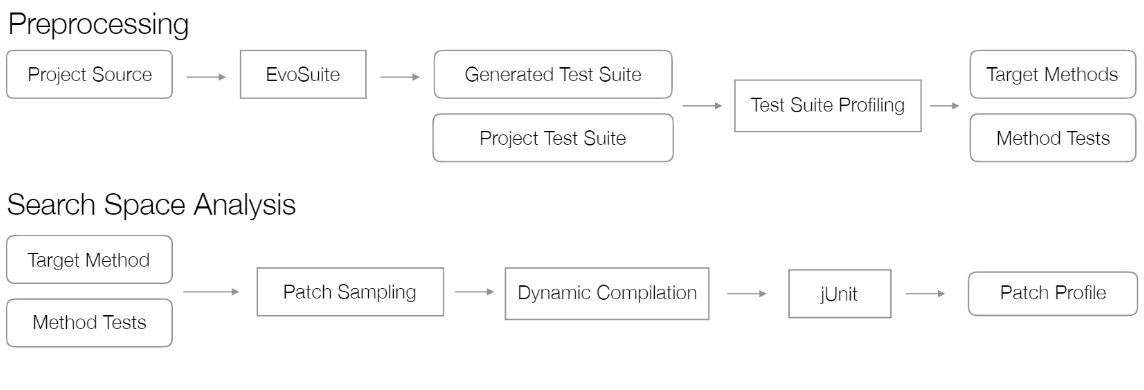
\includegraphics[width=1.0\textwidth]{img/Gin_Pipelines.png}
  \caption{Gin Pipelines from~\cite{DBLP:conf/gecco/BrownleePABWW19}}
  \label{fig:GinPipelines}
\end{figure}


As shown in Figure~\ref{fig:GinPipelines}, Gin provides two pipelines: \textit{Preprocessing} and \textit{Search Space Analysis}:\par

\vspace{.5em}
\textbf{Preprocessing}: Gin can preprocess a project and find the methods that are most likely to benefit from genetic improvement (GI). This is done by using the gin.util.Profiler class, which measures the execution time of each method in the project and ranks them by their contribution to the overall performance. The methods with the highest execution time are called 'hot methods' and are output as suitable targets for improvement by GI.\par

\vspace{.5em}
\textbf{Search Space Analysis}: Gin can also help to analyze the search space of possible program edits that can be applied by GI. The toolkit provides several tools that can sample and enumerate different types of edits, such as statement deletion, insertion, or replacement. These tools can be easily extended or reused to add new edit types. Gin will test each sampled or enumerated edit by applying it to the original code and running a test suite against the modified code. Gin will record various information about each edit, such as its validity (whether it preserves the functionality of the original code), its compilation result, its test output (whether it passes or fails the test suite), its run time (how long it takes to execute the test suite), and its error details (if any). Gin can use any test suite that is in JUnit format, which is a widely used testing framework for Java. Gin can also capture more detailed test output than just pass or fail, such as the difference between the expected and actual output. This allows Gin to support more fine-grained fitness functions that can measure the quality of each edit more accurately.\par


\begin{figure}[h]
  \centering
  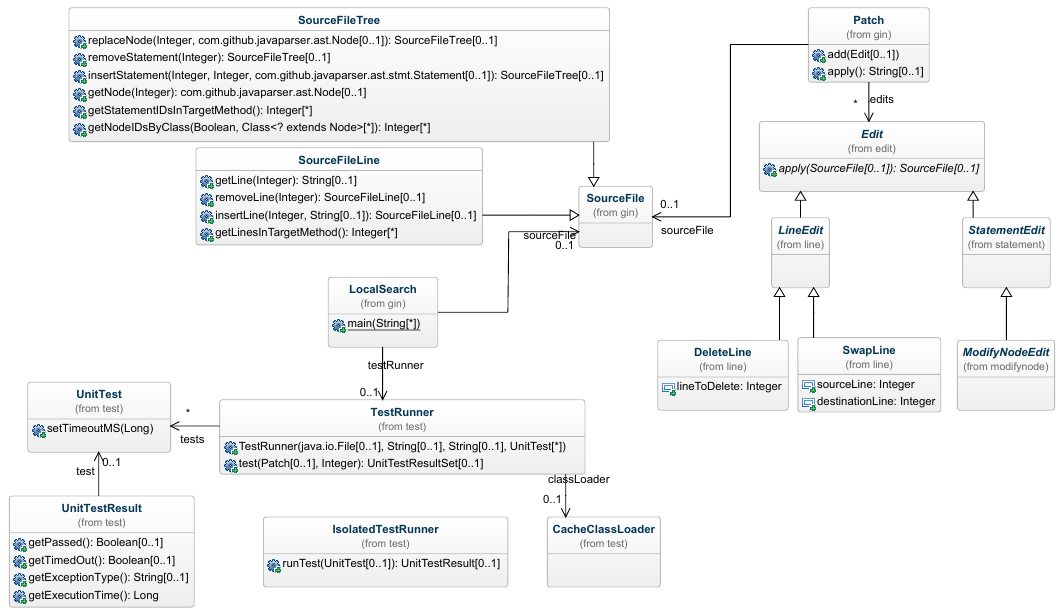
\includegraphics[width=.9\textwidth]{img/Ginclass.png}
  \caption{Gin Core Classes from~\cite{DBLP:conf/gecco/BrownleePABWW19}}
  \label{fig:Gin_Core_Classes}
\end{figure}

The Gin toolkit encompasses a collection of classes mentioned in Figure \ref{fig:Gin_Core_Classes} designed to facilitate genetic improvement research by offering a framework for manipulating source code, executing tests, and analyzing outcomes. At the core of this toolkit lies the SourceFile class, an immutable representation of the original source code, equipped with various methods for modifying the codebase, accessing language constructs, and generating modified Java source code.\par

\vspace{.5em}
Derived from the SourceFile class, the SourceFileTree subclass focuses on edits to the Abstract Syntax Tree (AST) of the source code. It assigns unique identifiers to each node within the AST, enabling efficient resolution of patches that entail multiple edits to the same location. In a similar vein, the SourceFileLine subclass directs its attention to line-level edits, also employing unique IDs for each line to simplify edit application.\par

\vspace{.5em}
A crucial component within Gin is the Patch class, which serves as a container for a series of edits, encapsulating the desired changes to be applied to the source code. The Edit class, serving as the base class for different types of edits, represents the application of a specific operator to the target source code. Subclasses of Edit, including LineEdit and StatementEdit, offer a range of operations for manipulating lines of code and modifying statements, respectively. The granularity of these edits provides fine-grained control over the code transformations.\par

\vspace{.5em}
To explore the search space of software transformations, the LocalSearch class employs a combination of sampling and searching techniques. It navigates through possible modifications to improve the code, ultimately enhancing its quality and performance. Meanwhile, the TestRunner class utilizes the JUnit framework to execute unit tests, offering insights into the outcomes, execution time, and encountered errors of the modified code.\par

\vspace{.5em}
The UnitTest class represents an individual unit test and is employed by the TestRunner to evaluate the test outcomes. Storing the result of a unit test, including pass/fail status, expected and actual results, and error details, the UnitTestResult class aids in analyzing the impact of code modifications on test behavior.\par

\vspace{.5em}
For focused testing of individual edits or patches, the IsolatedTestRunner subclass of TestRunner conducts tests in isolation. Finally, the CatcheClassLoader class, a custom ClassLoader, loads the modified class during test execution, overlaying the existing class hierarchy and facilitating the loading of the modified class by JUnit.\par

\vspace{.5em}
Collectively, these classes and their interplay within the Gin toolkit provide researchers with a powerful foundation for genetic improvement studies. The toolkit simplifies the process of editing source code, conducting tests, and evaluating the effects of modifications, thereby enabling more efficient and effective research in this domain. \par

\subsection{Identify the element need to be extended in the Gin tool}

In the previous subsection \ref{subsection:Gin_Tool}, we mentioned that the Gin tool comprises a collection of classes. Among these classes, the Edit class serves as the base class for different types of edits, representing the application of specific operators to the target source code. The subclasses of Edit, namely LineEdit and StatementEdit, offer a range of operations for manipulating lines of code and modifying statements, respectively. Based on the information mentioned above, it can be concluded that code refactoring techniques can be integrated into the genetic improvement tool, Gin Tool.

\begin{figure}[ht!]
  \centering
  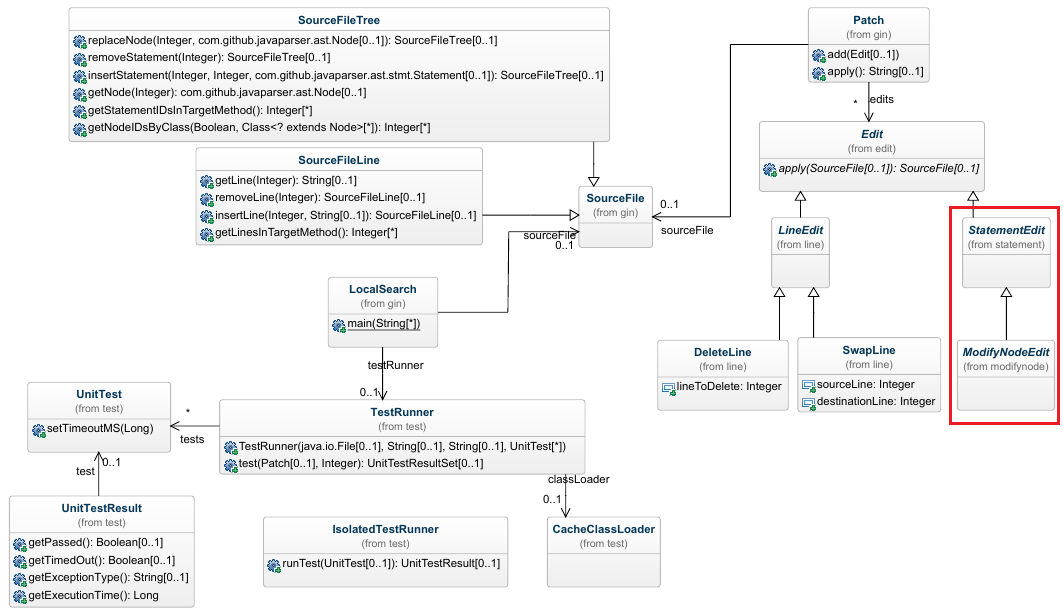
\includegraphics[width=.9\textwidth]{img/Gin_Core_Classes_extentions.png}
  \caption{Extension of the Gin Tool's class.~\cite{DBLP:conf/gecco/BrownleePABWW19}}
  \label{fig:Gin_Core_Classes_Extension}
\end{figure}

\vspace{.5em}
According to the information provided, the Edit class in the Gin tool acts as the base class for different types of edits and has two subclasses, LineEdit (providing a variety of operations for manipulating lines of code) and StatementEdit (offering a range of operations for modifying statements). Consequently, we have identified the StatementEdit class as the appropriate class for integrating selected code refactoring techniques. As StatementEdit offers a range of operations for modifying statements, and code refactoring techniques are closely related to statement edits, we consider StatementEdit to be the suitable class for incorporating code refactoring techniques. This integration will aid in obtaining the best patch, indicating an improved version of the program that consumes less energy.

\vspace{1em}
Figure \ref{fig:Gin_Core_Classes_Extension} below illustrates the identified class of the Gin tool where we will integrate the selected code refactoring techniques.



\section{Conclusion}
Through a comprehensive literature review, it has been observed that while various code refactoring techniques can improve software performance, their impact on energy efficiency varies based on the software's specific context. Notably, techniques like 'Convert Local Variable to Field', 'Introduce Parameter Object', and others have shown promise in reducing energy consumption. The Genetic Improvement (GIN) tool, which leverages Genetic Programming for software enhancement, presents an ideal platform to integrate these techniques. The StatementEdit class within GIN appears to be the most fitting for this integration, paving the way for potentially higher software quality and energy efficiency. This study effectively addresses the research question, highlighting the potential synergies between refactoring techniques and the GIN tool. Based on this analysis, we can answer research question \textbf{RQ2.2}: Code refactoring techniques can indeed be integrated into the Genetic Improvement tool, Gin. For this integration, the StatementEdit class in Gin will need to be extended. 


\chapter{Preliminary study for empirical evaluations}
\label{ch:prem_study}
%\section{Experimental executions using JoularJX}
%\label{sec:Experimental executions using JoularJX}

Our main objective is to reduce energy consumption in software using architectural software tactics. In order to delve deeper into this subject, it is essential to gain a comprehensive understanding of how we can measure the energy consumption of a program or project.

\vspace{.5em}
As mentioned, \textit{JoularJX} is a tool that can be used to monitor the energy consumption of a Java program or project at the method level. It can be hooked to the Java Virtual Machine when starting a Java program and provides real-time power consumption data for every method in the monitored program.

\vspace{.5em}
For our experiments, JoularJX was installed following the guidelines on \url{https://github.com/joular/joularjx}. We use version 2.0 of JoularJX, which requires a minimum of Java 11+ to run. On Windows, it depends on the Intel Power Gadget API, and on GNU/Linux, it uses the Intel RAPL interface through powercap.

\vspace{.5em}
All the experiment in this report were conducted on Dell Latitude 7490 laptop (Intel Core i7-8650U CPU @ 1.90GHz) running Debian GNU/Linux 11 (bullseye), Java 17 and JoularJX 2.0.

\vspace{.5em}
%As part of our research experiment, 
We conducted two preliminary experiments using JoularJX. These experiments are detailed as follows:

%a tool for monitoring energy consumption at the source code level:
%\begin{itemize}
%  \item \textbf{Energy consumption monitoring of a single java program (mandelbrot.java) using JoularJX.}
%  \item \textbf{Energy consumption monitoring of a project (cMath\_original) using JoularJX.}
%\end{itemize}
%Now, we will explain detail about the experiments conducted as part of our research.


%\section{Energy consumption monitoring of mandelbrot program using JoularJX}

\vspace{-10pt}
\section{Energy consumption monitoring of a single Java program}
\label{subsec: mandelbrot java program}

In this experiment, the energy consumption of a single Java program, \ie \texttt{mandelbrot}\footnote{\texttt{mandelbrot} was taken from the bench-marking used in~\cite{pereira2017energy},~\cite{couto2017towards}and~\cite{lima2016haskell} \url{http://benchmarksgame.alioth.debian.org/}} java program, was monitored using \textit{JoularJX~2.0}. 
To do that, a bash script named \texttt{jx\_script.sh} was created. 
The script created directories to organize the results and ran the Java program with different parameters for 30 iterations with the JoularJX agent attached. 
Then, 
%It included several Python files for data collection and analysis.
it sequentially executes the following Python files (see Appendix~\ref{sec:mainscript} for more details): 
\begin{enumerate}
    \item \texttt{jx\_gatherData.py}: reads energy and power data from CSV files in specific directories and created Pandas dataframes to store the data. The dataframes were then processed to extract relevant information (such as method names, parameters, iterations, and energy/power consumption), and this information was stored in lists. The lists were then used to create new dataframes with meaningful column names, which were then saved to CSV files. 
    \item \texttt{jx\_process\_level\_methods.py}: reads data from a CSV file containing energy and power consumption values for different iterations of a process. It then calculated the total and average energy consumption, and total and average power consumption for each process, and wrote these results to a new CSV file. The code used the \texttt{Python CSV} module to read and write CSV files and stored the results in dictionaries. 
    %The "jx\_process\_level\_methods.py" script analyzed the power consumption data at the method level, calculating energy and power for each method. 
    \item \texttt{jx\_plot.py}: generates graphs based on the gathered data. It creates box plots to visualize the total energy consumption and power consumption across all process IDs. 
    \item \texttt{shapiro\_wilk\_test\_energy.py and shapiro\_wilk\_test\_power.py}: performes \texttt{Shapiro-Wilk} tests to verfy the type of distribution, \ie normal or non- normal distributions, 
    %check for normality 
    in the energy and power consumption data.\par
\end{enumerate}

%"jx\_gatherData.py," "jx\_plot.py," "jx\_process\_level\_methods.py," "shapiro\_wilk\_test\_energy.py," and "shapiro\_wilk\_test\_power.py.".
%The script created directories to organize the results and ran the Java program with different parameters for 30 iterations with the JoularJX agent attached. 
%JoularJX collected energy and power consumption data, which was then processed and analyzed using the Python scripts. The "jx\_plot.py" script generated graphs based on the gathered data, and Shapiro-Wilk tests were performed to check for normality in the energy and power consumption data. The experiment was carried out by first cloning the repository from \url{https://gitlabev.imtbs-tsp.eu/sticamsud/enact-internship-2023.git}. Once cloned, the directory was changed to \texttt{enact-internship-2023/Code/Prem\_Experiment}. 


%In this experiment, we monitored the energy consumption of a single Java program, mandelbrot.java using JoularJX. We used JoularJX 2.0 version to obtain updated tree structure results in the output directory. To execute the Java program with JoularJX, we prepared a bash script named "jx\_script.sh", which includes several Python files: "jx\_gatherData.py," "jx\_plot.py," "jx\_process\_level\_methods.py," "shapiro\_wilk\_test\_energy.py," and "shapiro\_wilk\_test\_power.py.". Now, we will explain how the script works to collect the data of energy consumption of the program (mandelbrot.java).\par

%The script began by checking if a single argument, which was expected to be the name of the program without the file extension, was provided. If not, an error message was displayed. Then, a series of directories were created to organize the results. These directories included "jx\_results" as the main folder, which contained subfolders for "energy", "energy\_filtered", "power", and "power\_filtered". Each of these subfolders further contained "methods" and "calltrees" directories.\par

%Next, the script created a directory named "mandelbrot\_bitmap". The script then entered a loop where it ran the Java program with different parameters (15000, 20000, 30000, and 40000) for a certain number of iterations (30 in this case). The program was run with the JoularJX agent attached, which collected energy and power consumption data. For the first iteration, the program's output was saved as "mandelbrot\_bitmap/java\_temp.pmb".\par

%After each execution, four types of files were created by JoularJX, representing energy and power data at different levels of granularity. These files had specific names based on the process ID of the Java program. The script then moved the non-empty files to their respective directories under "jx\_results". If a file was empty, it was deleted.\par

%Once the iterations were completed, the script proceeded to execute Python scripts for further data processing and analysis. The script "jx\_gatherData.py" read energy and power data from CSV files in specific directories and created Pandas dataframes to store the data. The dataframes were then processed to extract relevant information (such as method names, parameters, iterations, and energy/power consumption), and this information was stored in lists. The lists were then used to create new dataframes with meaningful column names, which were then saved to CSV files. After that,  
%the "jx\_process\_level\_methods.py" script read data from a CSV file containing energy and power consumption values for different iterations of a process. It then calculated the total and average energy consumption, and total and average power consumption for each iteration, and wrote these results to a new CSV file. The code used the Python CSV module to read and write CSV files and stored the results in dictionaries. The "jx\_process\_level\_methods.py" script analyzed the power consumption data at the method level, calculating energy and power for each method. 
%The "jx\_plot.py" script generated graphs based on the gathered data. Subsequently, the "jx\_plot\_geom\_boxplot.py" script created box plots to visualize the total energy consumption across all process IDs. 

%Lastly, the script ran the "shapiro\_wilk\_test\_energy.py" and "shapiro\_wilk\_test\_power.py" scripts, which performed Shapiro\-Wilk tests to check for normality in the energy and power consumption data, respectively.\par
\vspace{-10pt}
\subsection{Experimental Results and Analysis} 

%In this section, we delve into the experimental findings on energy and power consumption of a Java program (\textit{mandelbrot}).

Figures \ref{fig:Shapiro-Wilk test results for Energy for mandelbrot} and \ref{fig:Shapiro-Wilk test results for Power for mandelbrot} shows the Shapiro-Wilk test outcomes for the gathered energy and power consumption.
%The Shapiro-Wilk test evaluates data normality; a high p-value suggests normal distribution while a low one indicates deviation. 
As seen, 
%For our data on "energy" and "power" (\textit{referenced in} figures \ref{fig:Shapiro-Wilk test results for Energy for mandelbrot} and \ref{fig:Shapiro-Wilk test results for Power for mandelbrot}), 
the obtained were \~0.843 and \~0.713, with \textit{p-values} of \(5.87 \times 10^{-10}\) and \(5.206 \times 10^{-14}\), respectively. Given these confident \textit{p-values} (less than 0.05), we can conclude that neither set of data follows a normal distribution.

%elucidating the distribution of energy and power data, respectively. 

%\vspace{-10pt}
%\setlength{\belowcaptionskip}{-10pt}
\begin{figure}[htbp]
  \centering
  \begin{minipage}[b]{.49\textwidth}
    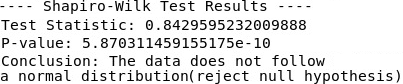
\includegraphics[width=1\linewidth]{img/mandelbrot_shapiro_test_energy_update.png}
    \caption{Shapiro-Wilk test results for Energy(\texttt{mandelbrot} program)}
    \label{fig:Shapiro-Wilk test results for Energy for mandelbrot}
  \end{minipage}
  \hfill
  \begin{minipage}[b]{0.49\textwidth}
    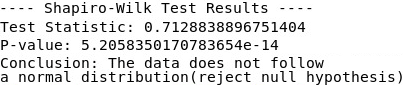
\includegraphics[width=1\linewidth]{img/mandelbrot_shapiro_test_power_update.png}
    \caption{Shapiro-Wilk test results for Power(\texttt{mandelbrot} program)}
    \label{fig:Shapiro-Wilk test results for Power for mandelbrot}
  \end{minipage}
\end{figure}
\vspace{-8pt}

Moreover, Figures \ref{fig:Graph of total energy consumption for mandelbrot} and \ref{fig:Graph of total power consumption for mandelbrot} 
%provide insights into the overall usage patterns. 
shows the box-plot for the data distribution of energy and power consumption of the processes
%IDs (PIDs) 
related to the execution of the java program.
%in Figure \ref{fig:Boxplot of total energy consumption for mandelbrot} enhances our understanding by highlighting potential outliers and data distribution. 
These visual aids collectively facilitate a comprehensive interpretation of the energy and power behaviors observed.
For instance, 
%a clear pattern emerges, 
we can observe four distinct clusters for energy consumption. It corresponds to the script parameter values, we used 15 000, 20 000, 30 000, and 40 000 as parameters of the \texttt{mandelbrot} code. A greater value for the parameter, a higher energy consumption values. Because at least the time is extended. Seeing the graph related to power consumption there is a more stable use of CPU for executing the \texttt{mandelbrot} code. These clusters were formed over 30 iterations. %highlighting the consistent energy and power usage patterns. 
%Interestingly, the energy and power consumption graphs show proportional clusters, indicating a direct relationship between the two metrics.

%In Figures \ref{fig:Graph of total energy consumption for mandelbrot} and \ref{fig:Graph of total power consumption for mandelbrot}, the energy and power consumption of Java processes are mapped against their unique Process IDs (PIDs) respectively. A clear pattern emerges, revealing four distinct clusters that correspond to script parameter values of 15,000, 20,000, 30,000, and 40,000. These clusters are formed over 30 iterations, highlighting the consistent energy and power usage patterns. Interestingly, the energy and power consumption graphs show proportional clusters, indicating a direct relationship between the two metrics.

\vspace{-12pt} % Reduce space above figure
\setlength{\belowcaptionskip}{-13pt} % Reduce space below caption
\begin{figure}[htbp]
  \centering
  \begin{center}
    \begin{minipage}[b]{0.49\textwidth}
      \centering
      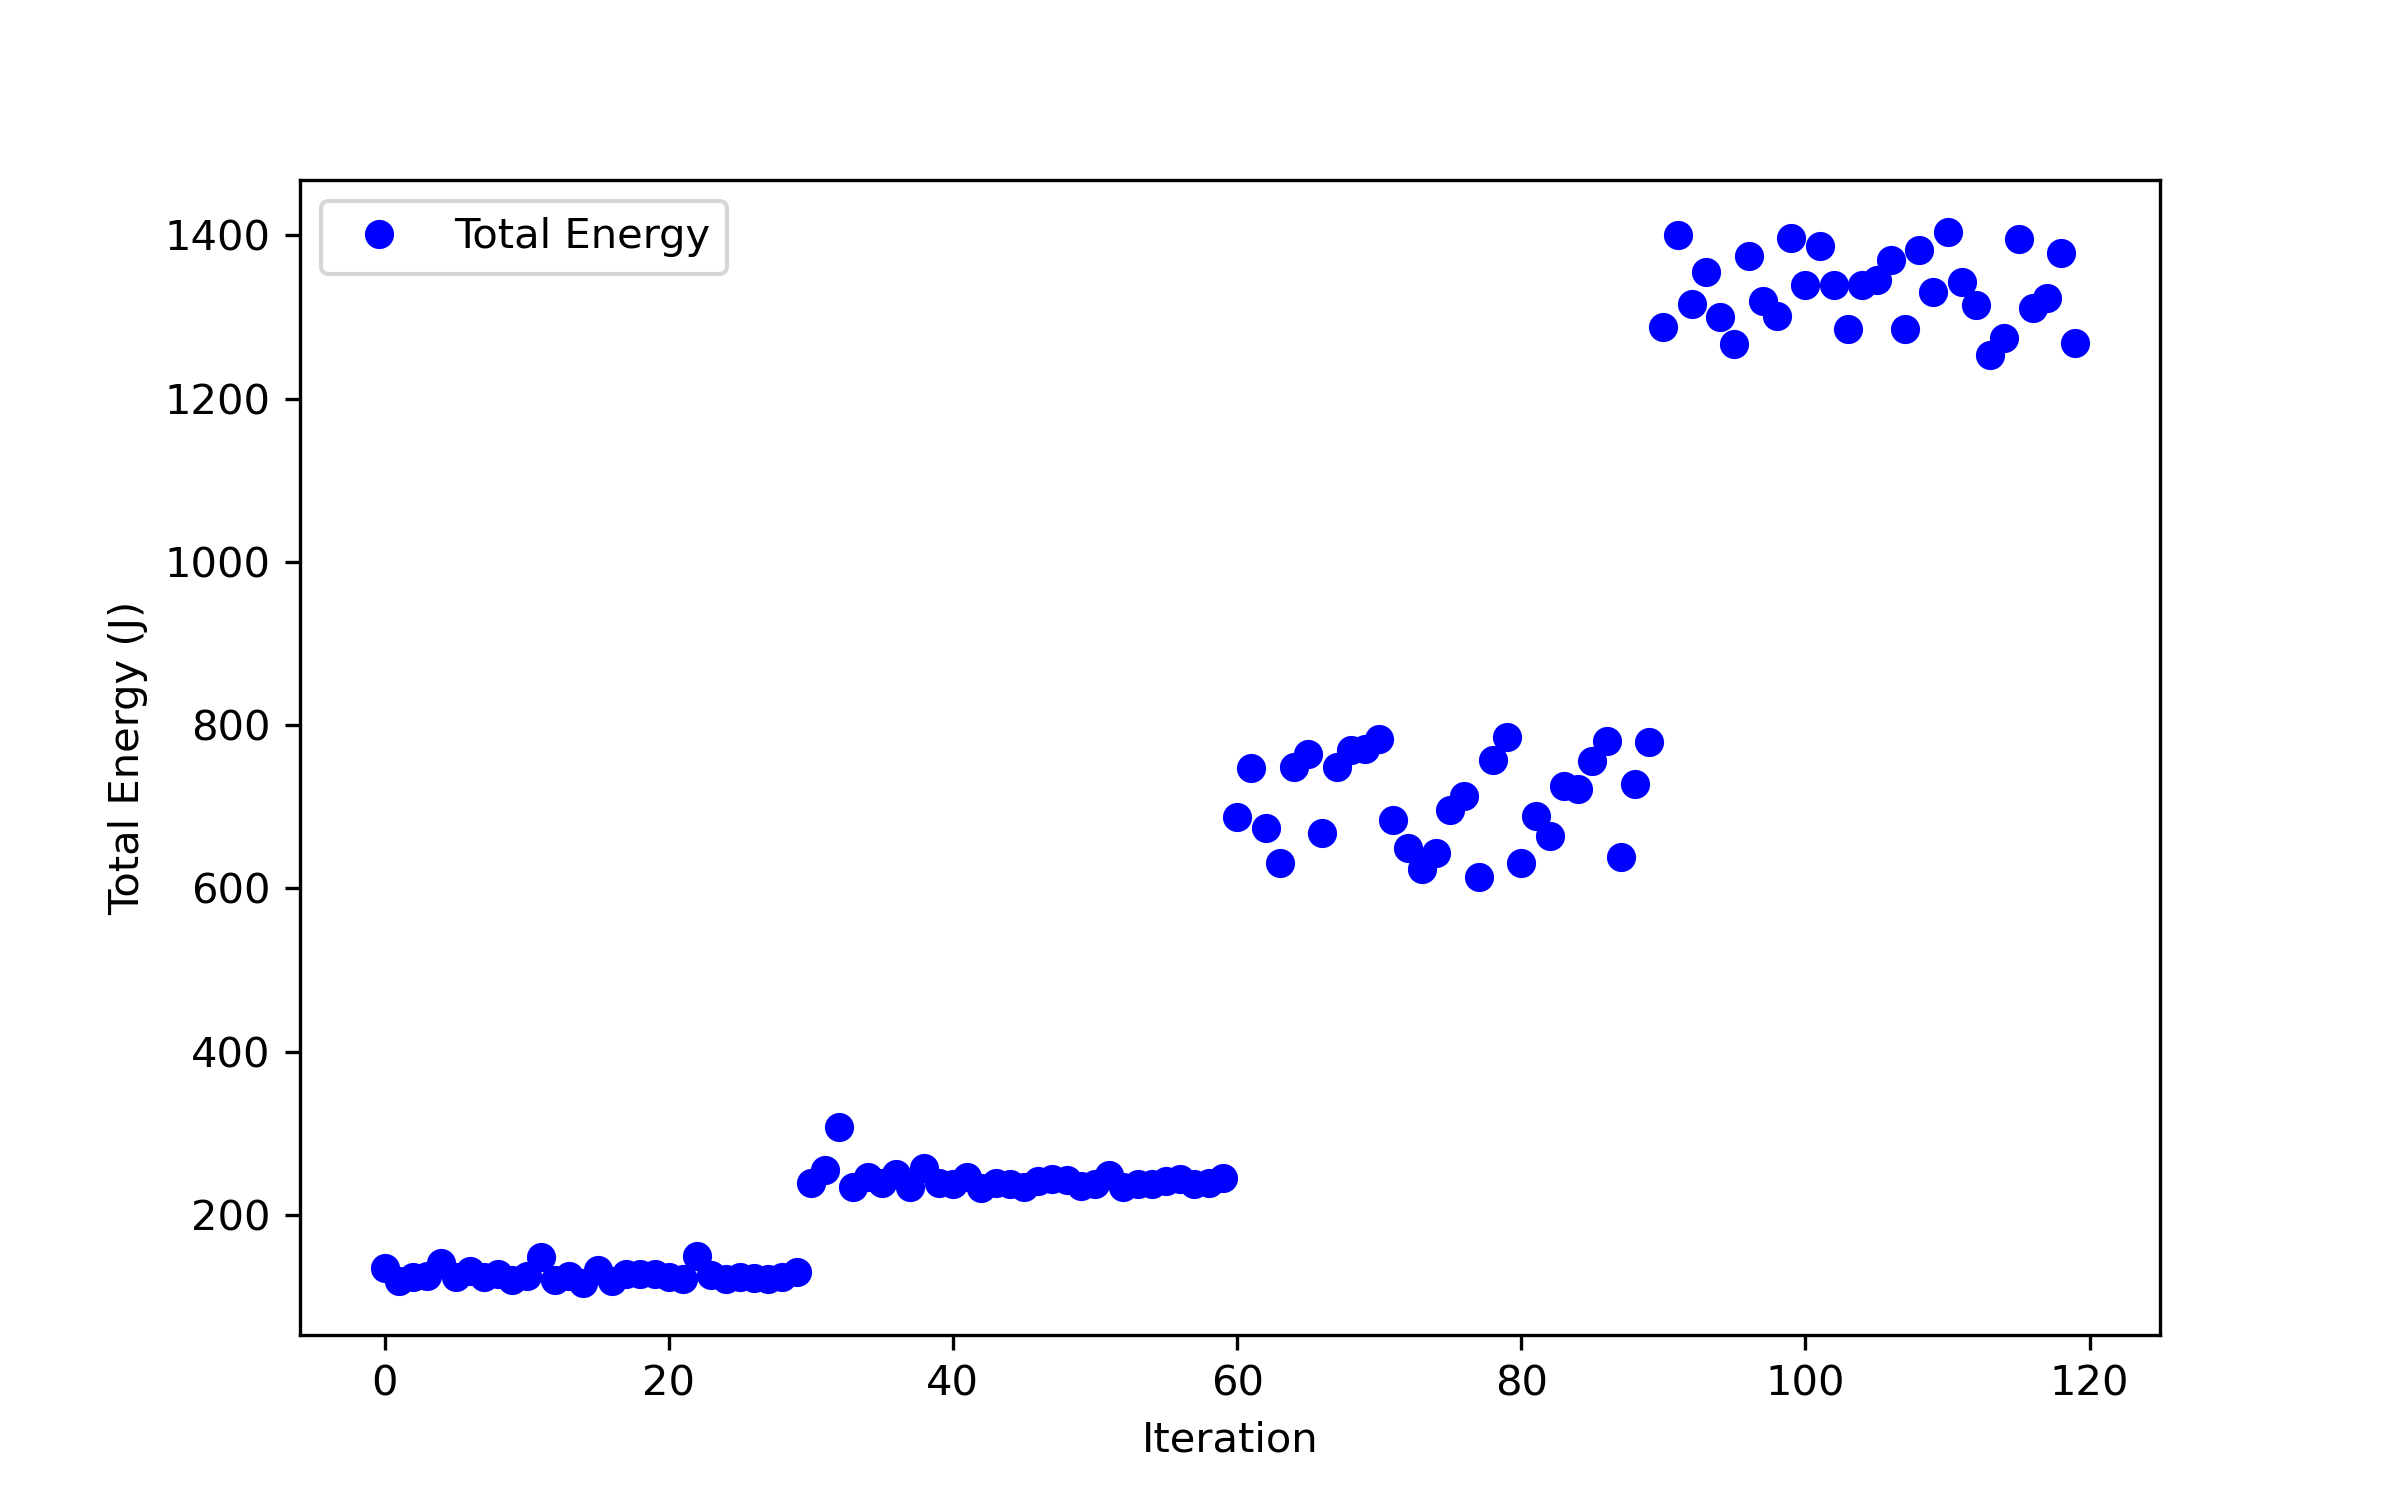
\includegraphics[width=\linewidth]{img/jx_total_energy_mandelbrot.png}
      \caption{Graph of total energy consumption(\texttt{mandelbrot} program)}
      \label{fig:Graph of total energy consumption for mandelbrot}
    \end{minipage}
    \hfill
    \begin{minipage}[b]{0.49\textwidth}
      \centering
      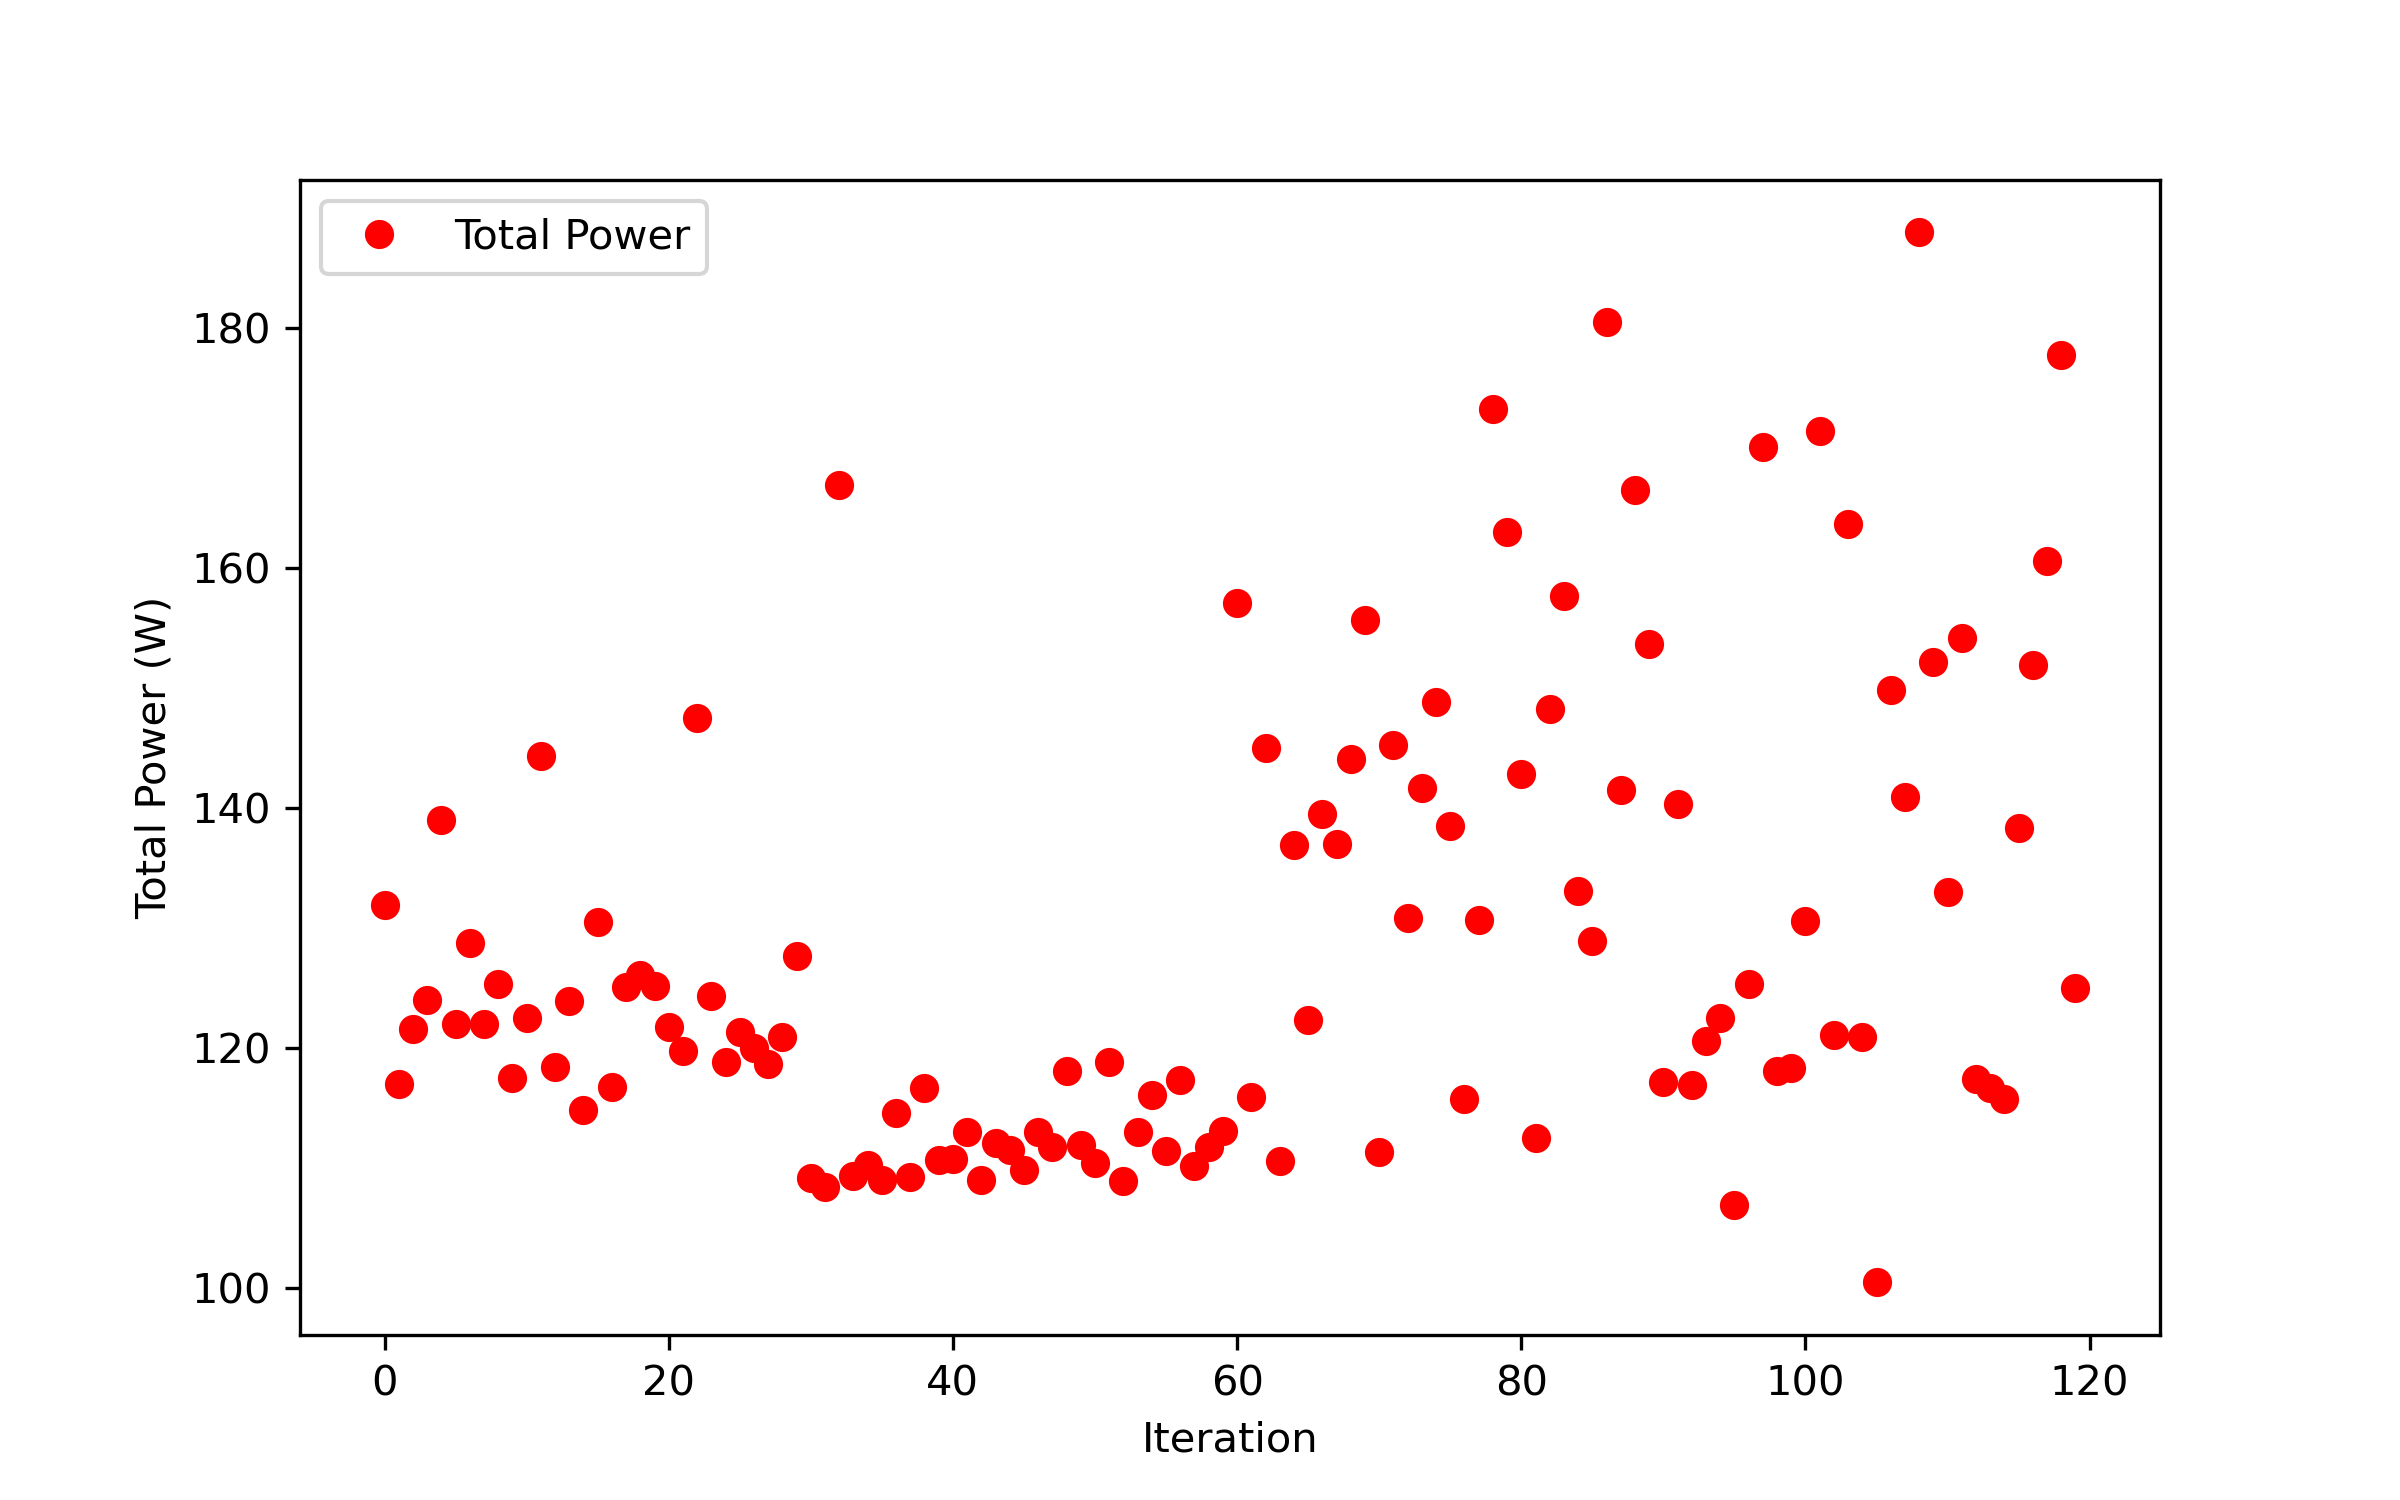
\includegraphics[width=\linewidth]{img/jx_total_power_mandelbrot.png}
      \caption{Graph of total power consumption(\texttt{mandelbrot} program)}
      \label{fig:Graph of total power consumption for mandelbrot}
    \end{minipage}
  \end{center}
\end{figure}
\vspace{-12pt} % Reduce space below figure


%\subsection{Energy consumption monitoring of a full project (cMath\_original) using JoularJX:} 
\vspace{-10pt}
\section{Energy consumption monitoring of a Java project} 

%In the second experiment, energy consumption for 'cMath\_original' was monitored using JoularJX 2.0. A test class, 'RunAllSuite.java', was executed using the \href{http://www.java2s.com/Code/Jar/c/Downloadcpsuite126jar.htm}{cpsuite-1.2.6.jar.zip} file and a script, 'jx\_script\_math.sh'. This script, containing various Python scripts, executed 'RunAllSuite.java' 30 times, managing resultant files in organized directories like "jx\_results". The Python scripts facilitated data extraction, processing, and graph generation from CSV files.The "shapiro\_wilk\_test\_energy.py" and "shapiro\_wilk\_test\_power.py" scripts assessed the normality of the energy and power data. The experiment was carried out by first cloning the repository from \url{https://gitlabev.imtbs-tsp.eu/sticamsud/enact-internship-2023.git} and navigating to the 'cMath\_original' directory within 'Prem\_Experiment'. After installation of JoularJX, as guided by its official website (\url{https://github.com/joular/joularjx}), the 'RunAllSuite.java' file located in 'src/test/java' was compiled. The resultant 'RunAllSuite.class' file was then moved to the 'bin' directory. The final step involved executing the 'jx\_script\_math.sh' script.


In the second experiment, the energy consumption of a Java project, \ie \texttt{cMath}\footnote{\texttt{cMath} was taken from the bench-marking used in~\cite{DBLP:conf/esem/SahinPC14} \url{https://bitbucket.org/udse/refactoring-study/src/master/} }, was monitored using \textit{JoularJX 2.0} as the previous experiment. 

\vspace{.5em}
%Similar to the previous experiment, \textit{JoularJX} was used to monitor energy and power consumption. %obtain updated tree structure results in the output directory. 
For a Java application, we execute its test cases classes that exercise the functionality of the Java application. The \texttt{cMath} application already contains a set of test cases classes. To execute all test cases of the project together, a new test class named \texttt{RunAllSuite.java} (see Appendix~\ref{sec:alltests} for more details) was created in the \texttt{test} directory. To execute the \texttt{RunAllSuite} class with JoularJX, it was necessary to download the \texttt{cpsuite-1.2.6}\footnote{\url{http://www.java2s.com/Code/Jar/c/Downloadcpsuite126jar.htm}} jar. 

\vspace{.5em}
A script called \texttt{jx\_script\_math.sh} in the \texttt{cMath} directory was created and used to execute the \texttt{RunAllSuite} class, which captured power and energy measurements using the JoularJX and managed the resulting files. 

%The script included several Python files: "jx\_gatherData.py," "jx\_plot.py," "jx\_process\_level\_methods.py," "shapiro\_wilk\_test\_energy.py," and "shapiro\_wilk\_test\_power.py." 

%The script set up directories for storing output files. These directories included "jx\_results" as the main folder, which contained subfolders for "energy", "energy\_filtered", "power", and "power\_filtered". Each of these subfolders further contained "methods" and "calltrees" directories.

\vspace{.5em}
The script sets the Java classpath for using the \textit{JUnit} and the \texttt{cpsuite-1.2.6} jars,  and performs the \texttt{RunAllSuite} java program in a loop for 30 iterations.
%
And, the script is based on the \texttt{jx\_script.sh} script (see Appendix~\ref{sec:mainscript}). So, the steps that it executes are the same than the previous experiment.

%During the first iteration, the output was saved to a file named 'java\_temp.pmb,' and for subsequent iterations, the output was discarded. After each execution, four types of files were created by JoularJX, representing energy and power data at different levels of granularity. These files had specific names based on the process ID of the Java program. The script then moved the non-empty files to their respective directories under "jx\_results". If a file was empty, it was deleted.

%Once the iterations were completed, the script proceeded to execute Python scripts for further data processing and analysis. The script "jx\_gatherData.py" read energy and power data from CSV files in specific directories and created Pandas data frames to store the data. The data frames were then processed to extract relevant information (such as method names, parameters, iterations, and energy/power consumption), and this information was stored in lists. The lists were then used to create new data frames with meaningful column names, which were then saved to CSV files. After that, the "jx\_process\_level\_methods.py" script read data from a CSV file containing energy and power consumption values for different iterations of a process. It then calculated the total and average energy consumption, and total and average power consumption for each process id, and wrote these results to a new CSV file. The code used the Python CSV module to read and write CSV files and stored the results in dictionaries. The "jx\_process\_level\_methods.py" script analyzed the power consumption data at the method level, calculating energy and power for each method. The "jx\_plot.py" script generated graphs based on the gathered data. Subsequently, the "jx\_plot\_geom\_boxplot.py" script created box plots to visualize the total energy consumption across all process IDs.

%Lastly, the script ran the "shapiro\_wilk\_test\_energy.py" and "shapiro\_wilk\_test\_power.py" scripts, which performed Shapiro\-Wilk tests to check for normality in the energy and power consumption data, respectively.\par

\subsection{Experimental Results and Analysis} 

In this section, we analyze the energy and power consumption data of the \textit{cMath} project. Figures \ref{fig:Shapiro-Wilk test results for Energy for cMath project} and \ref{fig:Shapiro-Wilk test results for Power for cMath project} depict the Shapiro-Wilk test results for energy and power data distributions. 
%These figures shed light on the distribution patterns of the data. 
%
%The Shapiro-Wilk test was performed on the data for "energy" and "power" from the cMath\_Original project to evaluate their normality. 
The test statistics obtained were $0.907$ and $0.864$ with \textit{p-values} of $0.013$ and $0.001$, respectively. Given these \textit{p-values} are below the $0.05$ significance level, we can reject the null hypothesis and conclude that the data for both measurements, \ie energy and power consumption, is not normally distributed.
%corroborated by visual assessments of their respective plots (figures \ref{fig:Shapiro-Wilk test results for Energy for cMath project} and \ref{fig:Shapiro-Wilk test results for Power for cMath project}).

\begin{figure}[h!]
  \centering
  \begin{minipage}[b]{0.49\textwidth}
    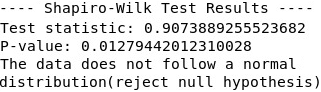
\includegraphics[width=.8\linewidth]{img/cMath_project_shapiro_test_energy_update.png}
    \caption{Shapiro-Wilk test results for Energy(\texttt{cMath} project)}
    \label{fig:Shapiro-Wilk test results for Energy for cMath project}
  \end{minipage}
  \hfill
  \begin{minipage}[b]{0.49\textwidth}
    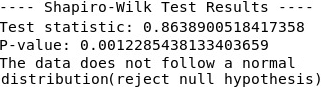
\includegraphics[width=.8\linewidth]{img/cMath_project_shapiro_test_power_update.png}
    \caption{Shapiro-Wilk test results for Power(\texttt{cMath} project)}
    \label{fig:Shapiro-Wilk test results for Power for cMath project}
  \end{minipage}
\end{figure}

%We also visually assess the overall consumption patterns using the graphs for total energy (Figure \ref{fig:Graph of total energy consumption for cMath project}) and power (Figure \ref{fig:Graph of total power consumption for cMath project}). A Boxplot analysis on the total energy consumption is presented in Figure \ref{fig:Boxplot of total energy consumption for cMath project} to highlight distribution and possible outliers.
\vspace{.5em}
Moreover, Figures \ref{fig:Graph of total energy consumption for cMath project} and \ref{fig:Graph of total power consumption for cMath project} shows the box-plot for the data distribution of energy and power consumption 
%represent energy and power consumption patterns against 
of process IDs (PID) from the execution of the Java application. The energy consumption varies between 1200 and 1320 joules with an average range of 1240 to 1320 joules, showing a noticeable spike between PIDs 54000 and 54500. Meanwhile, power consumption ranges from 10 to 80 Watts, averaging between 5 and 40 wards, with two notable peaks near 80 wards between PIDs 53500 and 54000. 
%These patterns help identify methods with high energy and power demands, which could benefit from optimization.

\begin{figure}[htbp]
  \centering
  \begin{center}
    \begin{minipage}[b]{0.49\textwidth}
      \centering
      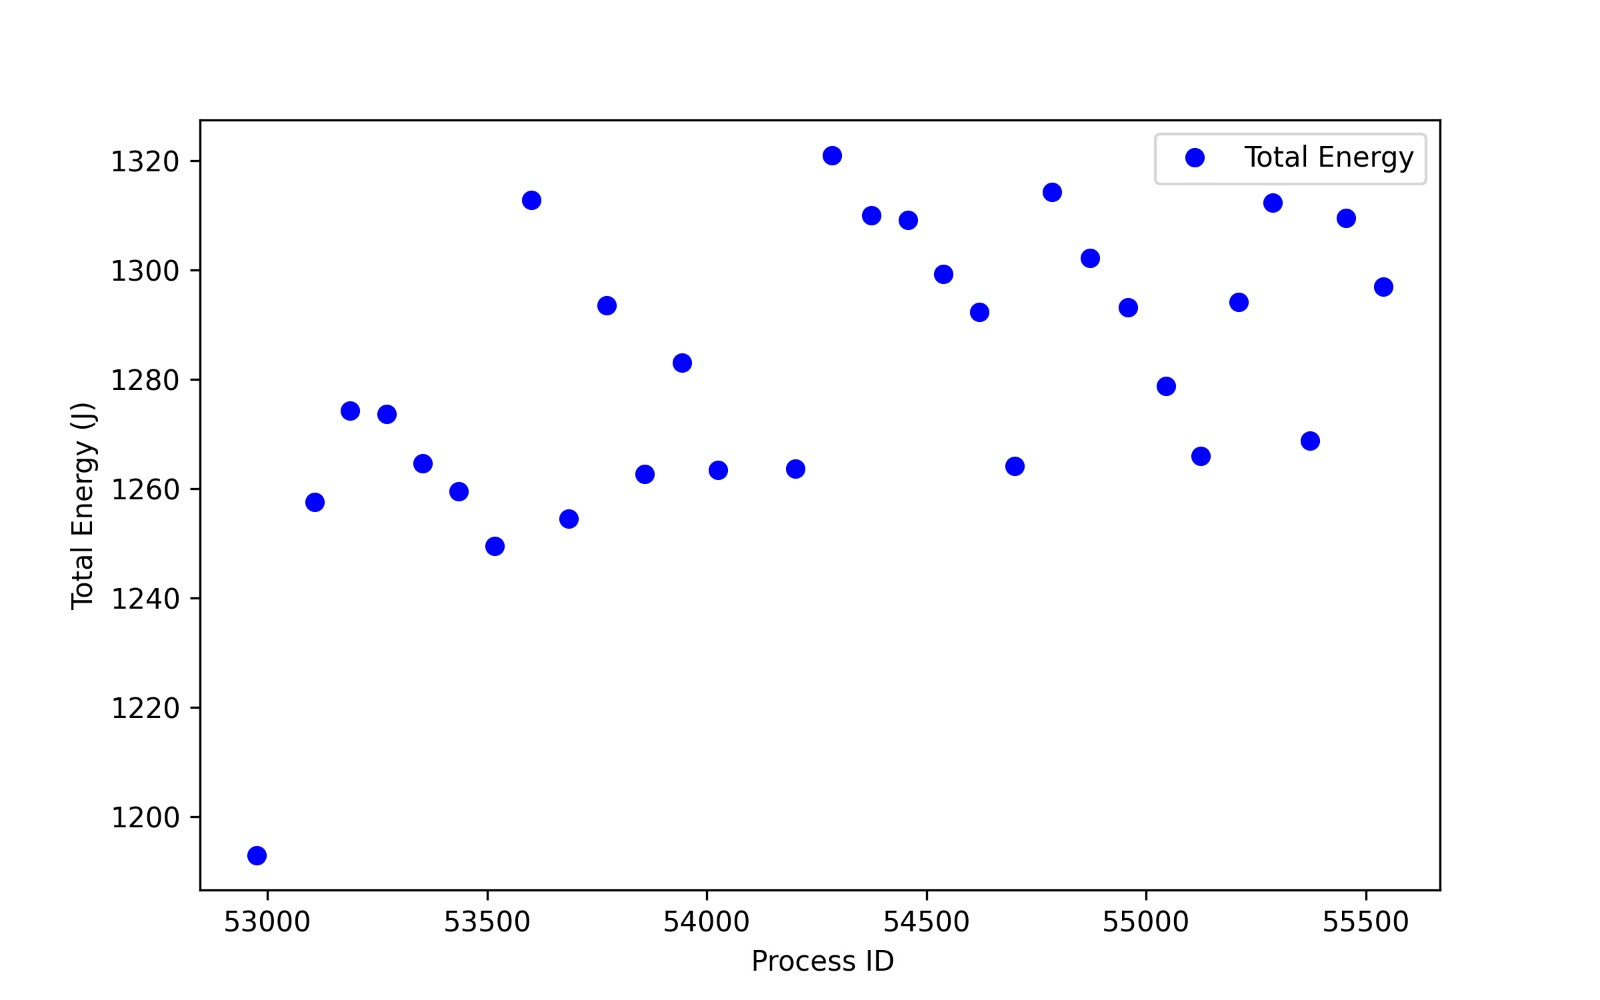
\includegraphics[width=\linewidth]{img/cMath_project_energy.jpeg}
      \caption{Graph of total energy consumption(\texttt{cMath} project)}
      \label{fig:Graph of total energy consumption for cMath project}
    \end{minipage}
    \hfill
    \begin{minipage}[b]{0.49\textwidth}
      \centering
      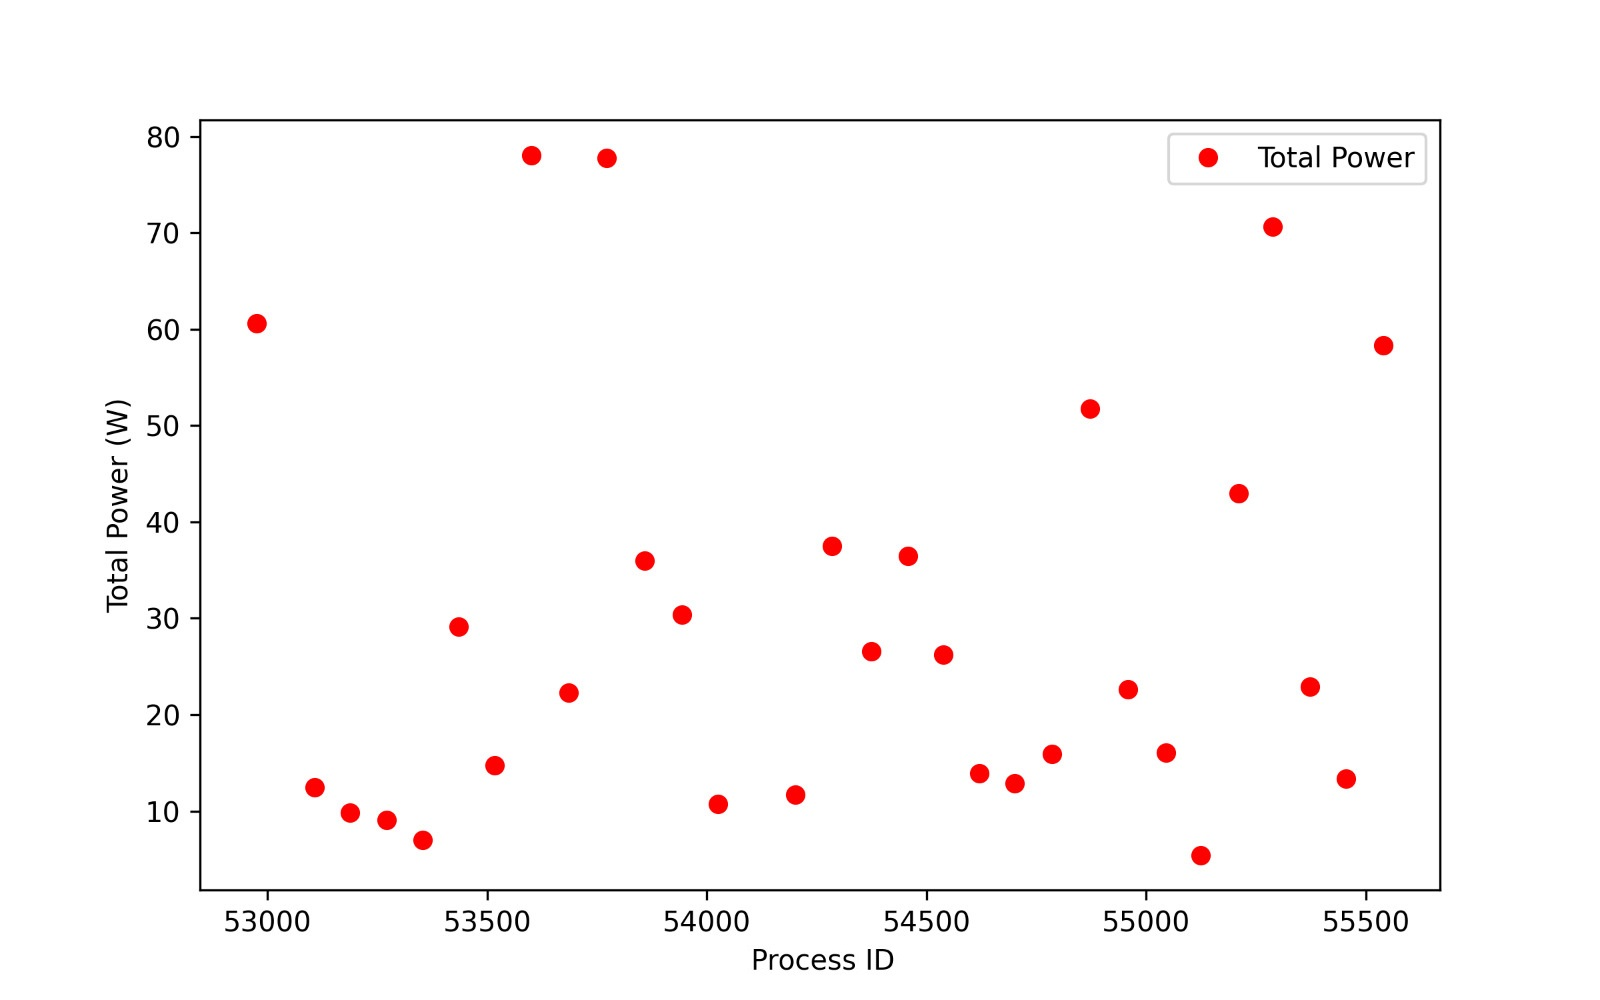
\includegraphics[width=\linewidth]{img/cMath_project_power.jpeg}
      \caption{Graph of total power consumption(\texttt{cMath} project)}
      \label{fig:Graph of total power consumption for cMath project}
    \end{minipage}
  \end{center}
\end{figure}

\vspace{10em}
In the analysis of the energy consumption for the \textit{cMath} project, as depicted in box-plot figure \ref{fig:Boxplot of total energy consumption for cMath project}, the proximity of the mean and median lines suggests a symmetric distribution, though the mean is slightly higher, hinting at some high consumption values. %Additionally, outliers on both sides of the whisker lines indicate unusual energy consumption values. 
This box-plot provides a comprehensive view of the project's typical energy usage, essential for its effective management.
\vspace{-10pt}
\begin{figure}[htbp]
  \centering
  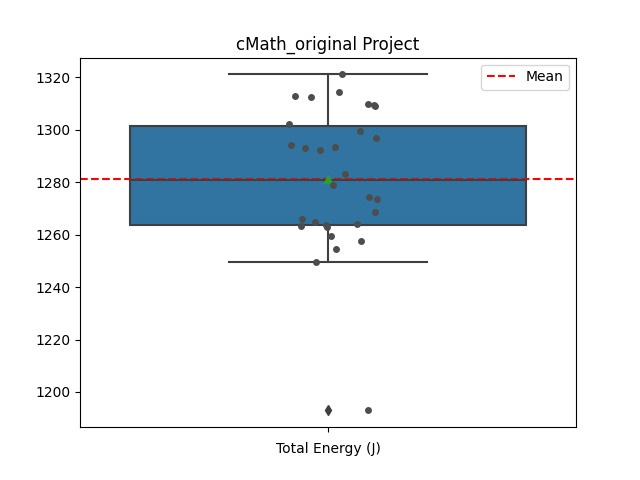
\includegraphics[width=.49\textwidth]{img/cMath_project_energy_boxplot.jpeg}
  \caption{Box-plot of total energy consumption(\texttt{cMath} project)}
  \label{fig:Boxplot of total energy consumption for cMath project}
\end{figure}
\vspace{-10pt}

\chapter{Proposal: Genetic Improvement toward Energy Efficiency}
\label{ch:solution}
In this chapter, we describe our proposal of using genetic improvement, \textit{i.e. the Gin toolbox}, for software energy efficiency. To do that, we investigate in which extent three fitness functions can reduce energy consumption.
Then, Next steps for integrating code refactoring to the gin toolbox are also provided in Section~\ref{sec:nextSteps} of Chapter~\ref{ch:conclusion}. %this preliminary work is to integrate

\section{Tactics for reducing energy consumption}\label{sec:tactics}

%GI ... fitness function
When using the Gin tool to improve a method within a program, we need to determine the appropriate fitness function. This function will guide the optimization process, ultimately yielding an improved version of the selected method for the program.
%RQ2.1
Based on our research question \textbf{RQ2.1}, we selected two types of fitness functions. These are:

% Single criteria fitness function
  %Tactic 1: Minimising time execution 
  %Minimising memory consumption
% Multi criteria fitness function
  % Minimising time execution and minimising memory consumption
  
\begin{enumerate}
    \item Single criteria fitness function
    \begin{itemize}
        \item \textbf{Tactic 1:} Minimize Execution Time
            \begin{itemize}
             \item \textbf{Objective:} Reduce the execution time of the program. Using this tactic, the 'gin' tool will generate an optimal patch that corresponds to the shortest execution time. This approach ensures that the code associated with the optimal patch not only compiles successfully but also enhances the program's execution time performance.
             \end{itemize}

        \item \textbf{Tactic 2:} Minimize Memory Consumption
            \begin{itemize}
            \item \textbf{Objective:} Decrease the memory usage of the program. With this tactic, the 'gin' tool will produce an optimal patch leading to reduced memory consumption. This method ensures that the code linked with the optimal patch compiles successfully and improves the program's memory consumption performance. Gin’s default \texttt{LocalSearch} Java class was primarily designed for execution time minimization. Given our specific objective of memory consumption minimization, we made modifications to the \texttt{LocalSearch} class.(see Appendix~\ref{sec:LocalSearch_Memory} for more details of updated version of the \texttt{LocalSearch} class)
            \end{itemize}
    \end{itemize}
    \item Multi criteria fitness function
    \begin{itemize}
        \item \textbf{Tactic 3}: Minimising Execution Time and minimising Memory Consumption.
        \begin{itemize}
            \item \textbf{Objective:} Reduce both the execution time and the memory usage of the program concurrently. Using this tactic, the 'gin' tool will generate an optimal patch that strikes a balance between minimizing execution time and memory consumption. This strategy ensures that the code associated with the optimal patch compiles successfully and offers a harmonized improvement in both the program's execution time and memory consumption performance. We adapted Gin’s default \texttt{LocalSearch} Java class to minimize both execution time and memory consumption together (see Appendix~\ref{sec:LocalSearch_Time_Memory} for more details of updated version of the \texttt{LocalSearch} class). To achieve this, a unique scoring system was devised where both the execution time and memory usage for each patch are normalized and summed. This aggregated score acts as the objective function, with the goal being its minimization. Consequently, a lower score indicates better performance in terms of time and memory. Throughout its iterations, the \texttt{LocalSearch} class tests various patches on the source code, selecting and retaining the one that produces the lowest score, thus ensuring efficient code performance.
            \end{itemize}
    \end{itemize}
\end{enumerate}

\section{Experimental Study Design }
%In this section, we detail the experiments conducted using the Gin tool to obtain optimized versions of selected programs. 
As mentioned, the evaluations using Gin were based on single-criteria fitness functions such as \textit{minimizing execution time} and \textit{minimizing memory consumption}, as well as a multi-criteria fitness function related to \textit{minimizing execution time and memory consumption} at the same time. 

\vspace{.5em}
We selected three programs for our experiments: \textit{Triangle}, \textit{Greatest Common Divisor (GCD)}, and \textit{Rectangle}. 

\vspace{.5em}
After the three programs were optimized with Gin, we collect data of energy consumption for the original and optimized versions of these programs by using \textit{JoularJX}.
%we performed two additional experiments for each program to determine the energy consumption of both the original and optimized versions using joularJX. 
%These experiments aimed to compare the energy consumption of the optimized versions with that of their original versions. 
Then we compare data gathered from the optimised and original versions of java programs. 
%if any improvement in terms of energy consumption 
To determine any significant difference between the data, we used the \texttt{Wilcoxon} statistical Test because the data distribution is non-normal. 

\vspace{.5em}
From these results, we will be able to address \textbf{RQ2.1}, which will help us determine whether the optimized version of the program, using the gin tool, has a significant impact on the reduction of energy consumption.

\subsection{Experimental Procedure to use Gin}
%\subsubsection{Experimental procedures}
To run our experiments, we sequentially executed the following steps:

\begin{enumerate}

\item \textbf{Prerequisites:} Gin requires:
\begin{itemize}
\item JDK 17
\item Gradle (tested with version 8.0.2)
\item A number of dependencies, which can be downloaded manually or via Gradle (recommended)
\item For Maven projects: make sure the Java version is set to the same version as Gin's.
\end{itemize}

\item \textbf{Clone the Repository:} Start by cloning the repository using the following command:

\begin{verbatim}
git clone https://github.com/gintool/gin.git
\end{verbatim}

\item \textbf{Navigate to the examples Directory:} Change the directory to the project folder:
\begin{verbatim}
cd gin/examples/triangle
\end{verbatim}

\item \textbf{Compile the java class file (\eg TriangleTest.java) :} Compile the TriangleTest.java program by running the following command:
\begin{verbatim}
javac -cp /usr/share/java/junit4.jar:. TriangleTest.java
\end{verbatim}

\item \textbf{Navigate to the gin Directory:} Change the directory to the gin folder:
\begin{verbatim}
cd ../../
\end{verbatim}

\item \textbf{Build using gradle (alternatively import into any IDE, such as IntelliJ) :}
\begin{verbatim}
gradle build
\end{verbatim}

This will build and test Gin, and also create a fat jar at build/gin.jar containing all required dependencies.

Note: If the provided build command will not work use the following command below:
\begin{verbatim}
./gradlew clean build -x test copyToLib
\end{verbatim}

This will ensure a clean build by removing any existing build artifacts, compiles the source code, skips test execution, and then executes the custom copyToLib task, which carries out additional project-specific actions defined in the build script and also create a fat jar at build/gin.jar containing all required dependencies.


\item \textbf{Execute the local search on a simple example:}
\begin{verbatim}
java -jar build/gin.jar -f examples/triangle/Triangle.java -m 
"classifyTriangle(int,int,int)"
\end{verbatim}

Note: If the provided command for Running a Simple Example will not able to work, follow the below informations and execute the commands:
\begin{verbatim}
java -cp build/gin.jar:lib/junit-vintage-engine-5.9.2.jar gin.LocalSearch -f
examples/triangle/Triangle.java -m "classifyTriangle(int,int,int)"
\end{verbatim}
Note: In this command specified the location of the necessary JAR files.
\end{enumerate}


\section{Experimental Results using Gin}

\subsection{Triangle Program}
\label{sec:Triangle}
 
The \textit{Triangle} code classifies triangles, given their side lengths, into one of four categories: invalid, equilateral, isosceles, or scalene. By sorting the input sides and analyzing their relationships, the program identifies and returns the type of triangle.

\vspace{.5em}
Specifically, our goal was to enhance the performance of the \texttt{classifyTriangle} method within the \textit{Triangle} program (see Appendix~\ref{sec:triangle}). We targeted the three fitness criteria mentioned in Section~\ref{sec:tactics} to optimize the triangle code using Gin.
Then optimized and original versions of the \textit{Triangle} code are compare in terms of their energy consumption. 


\subsubsection{Single criteria Fitness Function: Tactic 1(Minimizing execution time)}

For the \textit{triangle} java code, we minimize its execution time by using the Gin toolbox. Figure~\ref{fig:Optimised program file of Triangle 1} shows the execution of Gin on the \textit{triangle} code. As seen, it provides information about each step of the local search execution. It started with a summary of the file and method being analyzed, followed by reporting the original execution time of the method. As Figure~\ref{fig:Optimised program file of Triangle 1} shows, the execution time for the original version of the \textit{triangle} java code was 1636120217ns.

%\vspace{1.5em}
\begin{figure}[ht!]
  \centering
  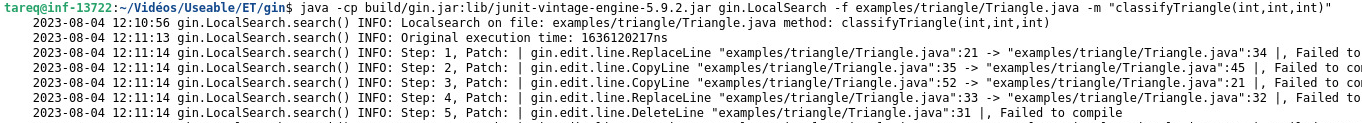
\includegraphics[width=1\textwidth]{img/Triangle_Experiment_output_1.png}
  \caption{Command line output: Optimized Triangle Java program with Gin tool.}
  \label{fig:Optimised program file of Triangle 1}
\end{figure}

\vspace{.5em}
For each step, the output indicated the patch being applied to the code. If a patch fails to compile, it means that the modified code could not be compiled successfully and this patch is discarded.If the patched code is complied and passes all provided tests, the execution time is calculated and showed if it better to previous version of code.

\begin{figure}[ht!]
  \centering
  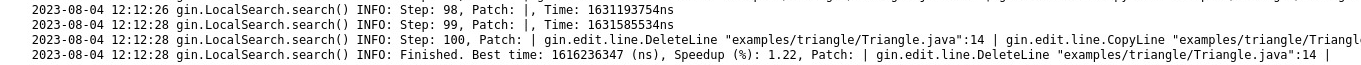
\includegraphics[width=1\textwidth]{img/Triangle_Experiment_output_2.png}
  \caption{Command line output: Optimized Triangle Java program with Gin tool.}
  \label{fig:Optimised program file of Triangle 2}
\end{figure}

\vspace{.5em}
The local search algorithm continued for a specified number of steps (condition for stopping  the Gin process), which was set to 100 by default (see Figure \ref{fig:Optimised program file of Triangle 2}). Throughout the process, different patches were generated and evaluated, aiming to find an optimized version of them.By examining the output, we could identify the patches that resulted in successfully compiled code and improved execution time. At the end of the process, a brief summary was provided to give an overview of the optimization results. Best time(Lowest execution time): 1616236347 (ns), Speedup (\%): 1.22.

\vspace{.5em}
Figure \ref{fig:Optimised program file of Triangle}
shows that the optimized code was generated. The figure displays the Optimised program file of the Triangle program in blue, representing the code that has been improved for better performance. Conversely, the green color represents the original program file of the Triangle program, which is the code in its initial state without any optimization.

\begin{figure}[ht!]
  \centering
  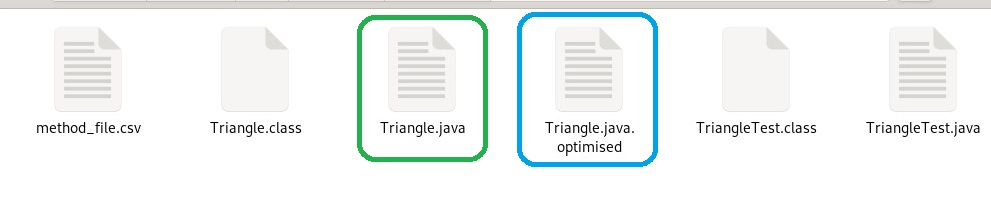
\includegraphics[width=.49\textwidth]{img/Triangle_Experiment_output.jpg}
  \caption{Optimised program file of Triangle}
  \label{fig:Optimised program file of Triangle}
\end{figure}



\subsubsection{Single criteria Fitness Function: Tactic 2(Minimizing memory consumption)}

For the \textit{triangle} java code, we minimize its memory consumption by using the Gin toolbox. Figure~\ref{fig:MC_2} shows the execution of Gin on the \textit{triangle} code. As seen, it provides information about each step of the local search execution. It started with a summary of the file and method being analyzed, followed by reporting the original memory consumption of the method. As Figure~\ref{fig:MC_2} shows, the memory consumption for the original version of the \textit{triangle} java code was 28 Mbytes.

\begin{figure}[htbp]
  \centering
  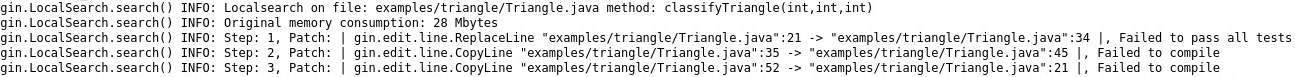
\includegraphics[width=1\textwidth]{img/Triangle_MC_2.png}
  \caption{Command line output: Memory Consumption Optimized Triangle Java program with Gin tool.}
  \label{fig:MC_2}
\end{figure}

\vspace{5em}
For each step, the output indicated the patch being applied to the code. If a patch fails to compile, it means that the modified code could not be compiled successfully and this patch is discarded. If the patched code is complied and passes all provided tests, the memory consumption is calculated and showed if it better to previous version of code.

\vspace{.5em}
The local search algorithm continued for a specified number of steps (condition for stopping  the Gin process), which was set to 100 by default (see Figure \ref{fig:MC_1}). Throughout the process, different patches were generated and evaluated, aiming to find an optimized version of them. By examining the output, we could identify the patches that resulted in successfully compiled code and improved memory consumption. At the end of the process, a brief summary was provided to give an overview of the optimization results. Best memory consumption: 22 Mbytes, Memory Consumption Reduction: 21.43\%.

\begin{figure}[htbp]
  \centering
  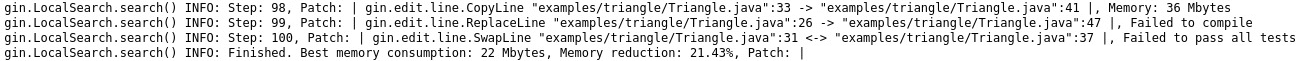
\includegraphics[width=1\textwidth]{img/Triangle_MC_1.png}
  \caption{Command line output: Memory Consumption Optimized Triangle Java program with Gin tool.}
  \label{fig:MC_1}
\end{figure}

\vspace{1em}
Finally, in the same directory where the original Triangle program is, the optimized code of Triangle program for memory consumption was generated based on the best patch that consumed the lowest memory.

\subsubsection{Multi criteria Fitness Function: Tactic 3(Minimizing execution time and memory consumption)}

For the \textit{triangle} java code, we minimize its execution time and memory consumption together by using the Gin toolbox. Figure~\ref{fig:EC_MC_1} shows the execution of Gin on the \textit{triangle} code. As seen, it provides information about each step of the local search execution. It started with a summary of the file and method being analyzed, followed by reporting the original execution time and memory consumption of the method. As Figure~\ref{fig:EC_MC_1} shows, the execution time and memory consumption for the original version of the \textit{triangle} java code was 1773092415 ns and 30 Mbytes.

\begin{figure}[htbp]
  \centering
  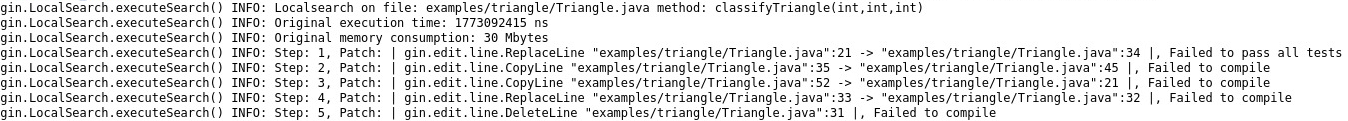
\includegraphics[width=1\textwidth]{img/Triangle_ET_MC_1.png}
  \caption{Command line output: Execution time and Memory Consumption Optimized Triangle Java program with Gin tool.}
  \label{fig:EC_MC_1}
\end{figure}

\vspace{.5em}
For each step, the output indicated the patch being applied to the code. If a patch fails to compile, it means that the modified code could not be compiled successfully and this patch is discarded.If the patched code is complied and passes all provided tests, the execution time and memory consumption are calculated and showed if it better to previous version of code.

\vspace{.5em}
The local search algorithm continued for a specified number of steps (condition for stopping  the Gin process), which was set to 100 by default (see Figure \ref{fig:Ec_MC_2}). Throughout the process, different patches were generated and evaluated, aiming to find an optimized version of them. By examining the output, we could identify the patches that resulted in successfully compiled code and improved execution time and memory consumption together. At the end of the process, a brief summary was provided to give an overview of the optimization results. Best time(Lowest execution time): 1751420953 (ns), Speedup (\%): 1.22, Best memory consumption: 26 Mbytes, Memory reduction: 13.33\%.

\begin{figure}[htbp]
  \centering
  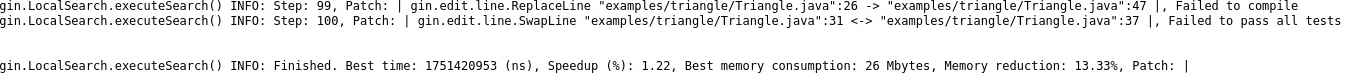
\includegraphics[width=1\textwidth]{img/Triangle_ET_MC_2.png}
  \caption{Command line output: Execution time and Memory Consumption Optimized Triangle Java program with Gin tool.}
  \label{fig:Ec_MC_2}
\end{figure}

\vspace{1em}
Finally, in the same directory where the original Triangle program is, the optimized code of Triangle program for execution time and memory consumption together was generated. This optimization was based on the best patch, which yielded the lowest memory consumption and lowest execution time.

\vspace{-10pt}
\subsection{Greatest Common Divisor(GCD) and Rectangle Program}

The \textit{GCD} Program computes the greatest common divisor (GCD) for three input integers. The fundamental purpose of this program is to determine the largest integer that can evenly divide all three numbers without leaving a remainder. To achieve this, the program utilizes the \texttt{findGCD} method.

\vspace{.5em}
The \textit{Rectangle} program categorizes a four-sided polygon based on its side lengths into one of three classifications: square, rectangle, or invalid shape. By evaluating the dimensions of the given sides, the program discerns the type of quadrilateral. If all four sides are the same length, it is identified as a square. If the opposite sides are equal, it is recognized as a rectangle. Conversely, if any side is non-positive or if the lengths don't fit the criteria for a square or rectangle, the shape is labeled as invalid. To achieve this, the program utilizes the \texttt{classifyRectangle}.

\vspace{.5em}
Specifically, our goal was to enhance the performance of the \texttt{findGCD} and \texttt{classifyRectangle} method within the \textit{GCD} and \textit{Rectangle} program (see Appendix~\ref{sec:GCD} and ~\ref{sec:rectangle}). We targeted the three fitness criteria mentioned in Section~\ref{sec:tactics} to optimize the triangle code using Gin. Then optimized and original versions of the \textit{GCD} and \textit{Rectangle} code are compare in terms of their energy consumption.

\vspace{.5em}
To optimize the two programs(\textit{GCD} and \textit{Rectangle}), using the Gin tool, we followed the same procedures as described for the \textit{Rectangle} program in Section~\ref{sec:Triangle}.

%In this section, we outline our experimental process designed to optimize the "Greatest Common Divisor (GCD)" Java program. Our primary focus was on enhancing the performance of the "findGCD" method within the program. We evaluated the optimization based on three distinct fitness criteria: "Execution Time," "Memory Consumption," and a combined criterion, "Combined Execution Time and Memory Consumption."

%\vspace{.5em}
%To initiate the experiment, we chose the "Greatest Common Divisor (GCD)\footnote{\url{https://gitlabev.imtbs-tsp.eu/sticamsud/enact-internship-2023/-/blob/main/Code/gin/Version_one_Execution_Time/gin/examples/GCD/GCD.java}}" program as our target program. This program's main function is to compute the greatest common divisor (GCD) of three provided integers. The `findGCD` method accepts these integers as parameters and returns their GCD in an efficient manner. Our experiments were based on the previously mentioned fitness criteria. The overarching goal was to bolster the program's efficiency by reducing its execution time, memory consumption, and a balance of both. To achieve these improvements, we used Gin's local search algorithm.

%\subsubsection{Single criteria Fitness: Execution time}

%In this experiment, our objective was to enhance the performance of the "findGCD" method within the "GCD" Java program. Our primary focus was to minimize its execution time. To achieve this, the program was executed using a specified command, and we applied Gin’s local search algorithm.

%\subsubsection{Experimental procedures}
%\begin{enumerate}

%\item \textbf{Prerequisites:} Gin requires:
%\begin{itemize}
%\item JDK 17
%\item Gradle (tested with version 8.0.2)
%\item A number of dependencies, which can be downloaded manually or via Gradle (recommended)
%\item For Maven projects: make sure the Java version is set to the same version as Gin's.
%\end{itemize}

%\item \textbf{Clone the Repository:} Start by cloning the repository using the following command:

%\begin{verbatim}
%git clone https://github.com/gintool/gin.git
%\end{verbatim}

%\item \textbf{Navigate to the examples Directory:} Change the directory to the project folder:
%\begin{verbatim}
%cd gin/examples/GCD
%\end{verbatim}

%\item \textbf{Compile the GCDTest.java file:} Compile the GCDTest.java program by running the following command:
%\begin{verbatim}
%javac -cp /usr/share/java/junit4.jar:. GCDTest.java
%\end{verbatim}

%\item \textbf{Navigate to the gin Directory:} Change the directory to the gin folder:
%\begin{verbatim}
%cd ../../
%\end{verbatim}

%\item \textbf{Build using gradle (alternatively import into any IDE, such as IntelliJ) :}
%\begin{verbatim}
%gradle build
%\end{verbatim}

%This will build and test Gin, and also create a fat jar at build/gin.jar containing all required dependencies.

%Note: If the provided build command will not work use the following command below:
%\begin{verbatim}
%./gradlew clean build -x test copyToLib
%\end{verbatim}

%This will ensure a clean build by removing any existing build artifacts, compiles the source code, skips test execution, and then executes the custom copyToLib task, which carries out additional project-specific actions defined in the build script and also create a fat jar at build/gin.jar containing all required dependencies.


%\item \textbf{Execute (running Gin's local search on a simple example) by running the following command:}
%\begin{verbatim}
%java -jar build/gin.jar -f examples/GCD/GCD.java -m 
%"findGCD(int,int,int)"
%\end{verbatim}

%Note: If the provided command for Running a Simple Example will not able to work, follow the below informations and execute the commands:
%\begin{verbatim}
%java -cp build/gin.jar:lib/junit-vintage-engine-5.9.2.jar gin.LocalSearch -f 
%examples/GCD/GCD.java -m "findGCD(int,int,int)"
%\end{verbatim}
%Note: In this command specified the location of the necessary JAR files.
%\end{enumerate}

%\subsubsection{Experimental Results and Analysis:}

%This section presents the experimental results and analysis of the optimization experiment conducted to achieve an optimized GCD Java program. The focus of the optimization was specifically on improving the "findGCD" method within the program, utilizing the Gin tool.

%\begin{figure}[htbp]
  %\centering
  %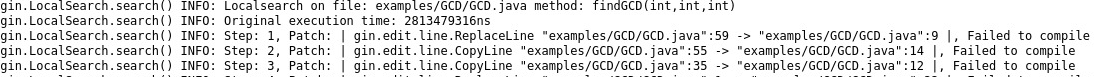
\includegraphics[width=1\textwidth]{img/GCD_ET_1.png}
  %\caption{Command line output:  Execution time Optimized GCD Java program with Gin tool.}
  %\label{fig:GCD_ET_1}
%\end{figure}


%The output(figure \ref{fig:GCD_ET_1}) of the program provided information about each step of the local search process. It started with a summary of the file and method being analyzed, followed by reporting the original execution time of the method.The  Original execution time was 2813479316 ns.

%\begin{figure}[htbp]
  %\centering
  %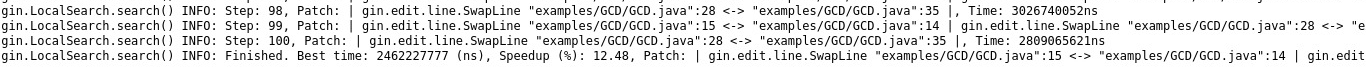
\includegraphics[width=1\textwidth]{img/GCD_ET_2.png}
 %\caption{Command line output:  Execution time Optimized GCD Java program with Gin tool.}
  %%\label{fig:GCD_ET_2}
%\end{figure}


%By examining the output(figure \ref{fig:GCD_ET_2}), we could able to identify the patches that resulted in successfully compiled code and improved execution time performance. The goal was to find the fastest code that passed all provided tests. At the end of the process, a brief summary was provided to give an overview of the optimization results. Best time(Lowest execution time): 2462227777 (ns), Speedup (\%): 12.48.

%\begin{figure}[htbp]
  %\centering
  %
\includegraphics[width=.7\textwidth]{img/GCD_ET_Folder.png}
  %\caption{Optimised program file of GCD program}
  %\label{fig:Optimised program file of GCD program}
%\end{figure}


%In Figure \ref{fig:Optimised program file of GCD program}, the directory where the optimized code was generated is specified. The figure displays the Optimised program file of the GCD program in blue, representing the code that has been improved for better performance. Conversely, the green color represents the original program file of the Triangle program, which is the code in its initial state without any optimization. This color distinction helps visually differentiate between the optimized and original versions of the code.

%\subsubsection{Single criteria Fitness: Memory Consumption}

%In our experiment, we aimed to optimize the memory consumption of the ``findGCD'' method in the ``GCD'' Java program using Gin's local search algorithm. Gin's default \texttt{LocalSearch} Java class was primarily designed for execution time minimization. Given our specific objective of memory consumption minimization, we made modifications to the \texttt{LocalSearch} class. The updated version of the class can be accessed at the \href{https://gitlabev.imtbs-tsp.eu/sticamsud/enact-internship-2023/-/blob/main/Code/gin/Version_two_Memory_Consumption/gin/src/main/java/gin/LocalSearch.java}{link}. Our experimental procedures followed the same experimental procedures of single-criteria fitness: execution time.

%\subsubsection{Experimental Results and Analysis:}
%In this section, we detail the optimization results for the "findGCD" method in the GCD Java program, specifically focusing on memory consumption. Using the Gin tool, the experiment showed that the method's original memory usage was 180 Mbytes, as seen in figure \ref{fig:GCD_MC_1}.

%\begin{figure}[htbp]
  %\centering
  %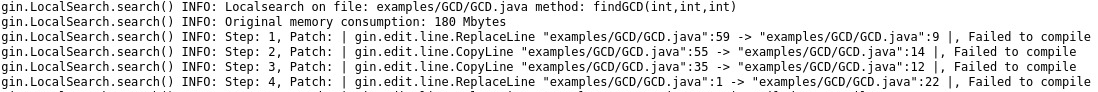
\includegraphics[width=1\textwidth]{img/GCD_MC_1.png}
  %\caption{Command line output: Memory Consumption Optimized GCD Java program with Gin tool.}
  %\label{fig:GCD_MC_1}
%\end{figure}

%\vspace{1em}
%By examining the output in figure \ref{fig:GCD_MC_2}, we were able to identify the specific patches that led to successfully compiled code with improved memory consumption performance. Our primary objective was to identify the best patch that consumed the least memory while passing all provided tests. In summary, the optimization results indicate the best memory consumption at 28 Mbytes, representing a reduction of 84.44\%.

%\begin{figure}[htbp]
  %\centering
  %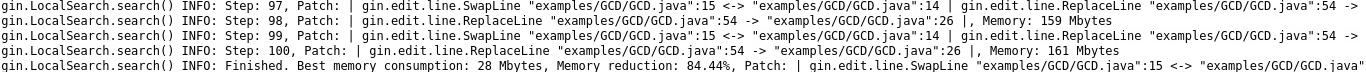
\includegraphics[width=1\textwidth]{img/GCD_MC_2.png}
  %\caption{Command line output: Memory Consumption Optimized GCD Java program with Gin tool.}
  %\label{fig:GCD_MC_2}
%\end{figure}

%\vspace{1em}
%Finally, in the same directory where the original GCD program is, the optimized code of GCD program for memory consumption was generated based on the best patch that consumed the lowest memory.

%\subsubsection{Multi criteria Fitness: Combined Execution time and Memory consumption}
%In our experiment, we aimed to optimize both the execution time and memory consumption together of the ‘findGCD’ method in the ‘GCD’ Java program using Gin’s local search algorithm. As Gin’s default ‘LocalSearch’ Java class was primarily designed for execution time minimization, we adapted it to minimize both execution time and memory consumption together. The updated version of the class can be accessed at the provided \href{https://gitlabev.imtbs-tsp.eu/sticamsud/enact-internship-2023/-/blob/main/Code/gin/Version_three_ExecutionTime_and_MemoryConsumption/gin/src/main/java/gin/LocalSearch.java}{link}. The LocalSearch class has been refined to optimize both memory consumption and execution time for patches. To achieve this, a unique scoring system was devised where both the execution time and memory usage for each patch are normalized and summed. This aggregated score acts as the objective function, with the goal being its minimization. Consequently, a lower score indicates better performance in terms of time and memory. Throughout its iterations, the LocalSearch class tests various patches on the source code, selecting and retaining the one that produces the lowest score, thus ensuring efficient code performance. Our experimental procedures followed the same procedures as single-criteria fitness for execution time

%\subsubsection{Experimental Results and Analysis:}

%In this section, we detail the optimization results for the "findGCD" method in the GCD Java program, specifically focusing on execution time and memory consumption together. Using the Gin tool, the experiment showed that the method's Original execution time: 2892005383 ns and Original memory usage was 158 Mbytes, as seen in figure \ref{fig:GCD_EC_MC_1}.

%\begin{figure}[htbp]
  %\centering
  %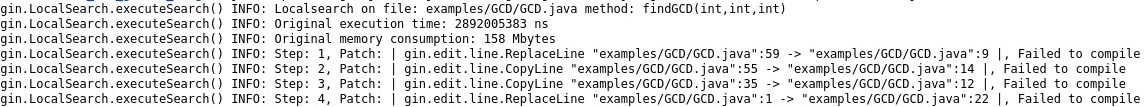
\includegraphics[width=1\textwidth]{img/GCD_ET_MC_1.png}
  %\caption{Command line output: Combined Execution time and Memory Consumption Optimized GCD Java program with Gin tool.}
 %\label{fig:GCD_EC_MC_1}
%\end{figure}

%By analyzing the output in figure \ref{fig:GCD_EC_MC_2}, we identified specific patches that resulted in a successful code compilation and enhanced both execution time and memory consumption performance. Our main goal was to find the most optimal patch one that sped up the program and consumed the least memory while still passing all the tests. In summary, the optimization results indicate the Best time: 2631710897 (ns), Speedup (\%): 9.00, Best memory consumption: 23 Mbytes, Memory reduction: 85.44\%.

%\begin{figure}[htbp]
  %\centering
  %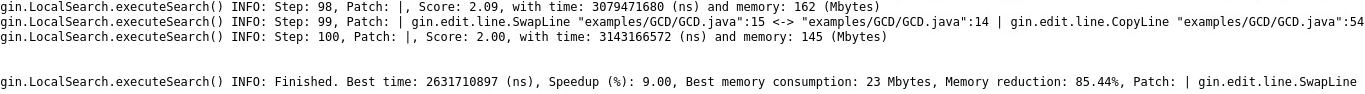
\includegraphics[width=1\textwidth]{img/GCD_ET_MC_2.png}
  %\caption{Command line output: Combined Execution time and Memory Consumption Optimized GCD Java program with Gin tool.}
  %\label{fig:GCD_EC_MC_2}
%\end{figure}

%\vspace{1em}
%Finally, in the same directory where the original GCD program is, the optimized code of GCD program for execution time and memory consumption together was generated. This optimization was based on the best patch, which yielded the lowest memory consumption and shortest execution time.



%\subsection{Rectangle Program Optimization using Gin Tool}

%In this section, we describe our experimental process, wherein we sought to optimize the "Rectangle" Java program. Specifically, our goal was to enhance the performance of the "classifyRectangle" method within this program. We targeted three distinct fitness criteria: two single criteria fitness "Execution Time," "Memory Consumption," and a multi-criteria fitness, "Combined Execution Time and Memory Consumption."

%\vspace{.5em}
%To begin the experiment, we selected the "Rectangle\footnote{\url{https://gitlabev.imtbs-tsp.eu/sticamsud/enact-internship-2023/-/blob/main/Code/gin/Version_one_Execution_Time/gin/examples/rectangle/Rectangle.java}}" program as our target.  The Rectangle program classifies a quadrilateral using its four side lengths into either a square, rectangle or an invalid shape. It deems the shape as a square if all sides are equal, a rectangle if opposite sides are identical, and invalid if any side is non-positive or if the sides don't conform to either the square or rectangle criteria. Our three experiments are grounded in the fitness criteria mentioned earlier. The ultimate objective was to enhance the program's efficiency, minimizing execution time, memory consumption, and the combination of both. We applied Gin's local search algorithm to achieve this. 


%\subsubsection{Single criteria Fitness: Execution time}
%In this experiment, our objective was to enhance the performance of the "classifyRectangle" method within the "Rectangle" Java program. Our primary focus was to minimize its execution time. To achieve this, the program was executed using a specified command, and we applied Gin’s local search algorithm.

%\subsubsection{Experimental procedures}
%\begin{enumerate}

%\item \textbf{Prerequisites:} Gin requires:
%\begin{itemize}
%\item JDK 17
%\item Gradle (tested with version 8.0.2)
%\item A number of dependencies, which can be downloaded manually or via Gradle (recommended)
%\item For Maven projects: make sure the Java version is set to the same version as Gin's.
%\end{itemize}

%\item \textbf{Clone the Repository:} Start by cloning the repository using the following command:

%\begin{verbatim}
%git clone https://github.com/gintool/gin.git
%\end{verbatim}

%\item \textbf{Navigate to the examples Directory:} Change the directory to the project folder:
%\begin{verbatim}
%cd gin/examples/rectangle
%\end{verbatim}

%\item \textbf{Compile the RectangleTest.java file:} Compile the RectangleTest.java program by running the following command:
%\begin{verbatim}
%javac -cp /usr/share/java/junit4.jar:. RectangleTest.java
%\end{verbatim}

%\item \textbf{Navigate to the gin Directory:} Change the directory to the gin folder:
%\begin{verbatim}
%cd ../../
%\end{verbatim}

%\item \textbf{Build using gradle (alternatively import into any IDE, such as IntelliJ) :}
%\begin{verbatim}
%gradle build
%\end{verbatim}

%This will build and test Gin, and also create a fat jar at build/gin.jar containing all required dependencies.

%Note: If the provided build command will not work use the following command below:
%\begin{verbatim}
%./gradlew clean build -x test copyToLib
%\end{verbatim}

%This will ensure a clean build by removing any existing build artifacts, compiles the source code, skips test execution, and then executes the custom copyToLib task, which carries out additional project-specific actions defined in the build script and also create a fat jar at build/gin.jar containing all required dependencies.


%\item \textbf{Execute (running Gin's local search on a simple example) by running the following command:}
%\begin{verbatim}
%java -jar build/gin.jar -f examples/triangle/Rectangle.java -m 
%"classifyRectangle(int,int,int,int)"
%\end{verbatim}

%Note: If the provided command for Running a Simple Example will not able to work, follow the below informations and execute the commands:
%\begin{verbatim}
%java -cp build/gin.jar:lib/junit-vintage-engine-5.9.2.jar gin.LocalSearch -f
%examples/rectangle/Rectangle.java -m "classifyRectangle(int,int,int,int)"
%\end{verbatim}
%Note: In this command specified the location of the necessary JAR files.
%\end{enumerate}

%\subsubsection{Experimental Results and Analysis:}

%This section presents the experimental results and analysis of the optimization experiment conducted to achieve an optimized Rectangle Java program. The focus of the optimization was specifically on improving the "classifyRectangle" method within the program, utilizing the Gin tool.

%\vspace{6em}
%\begin{figure}[htbp]
  %\centering
 % 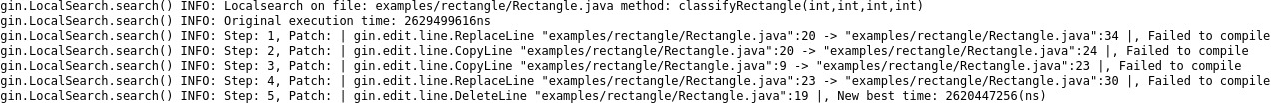
\includegraphics[width=1.\textwidth]{img/Rectangle_ET_1.png}
 % \caption{Command line output:Execution time Optimized %Rectangle Java program with Gin tool.}
 % \label{fig:Rectangle_ET_1}
%\end{figure}

%The output(figure \ref{fig:Rectangle_ET_1}) of the program provided information about each step of the local search process. It started with a summary of the file and method being analyzed, followed by reporting the original execution time of the method.The  Original execution time was 2629499616 ns.

%\begin{figure}[htbp]
  %\centering
  %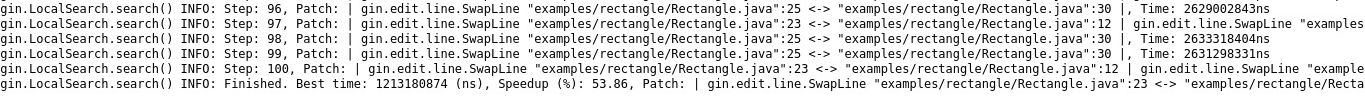
\includegraphics[width=1.\textwidth]{img/Rectangle_ET_2.png}
  %\caption{Command line output:Execution time Optimized %%Rectangle Java program with Gin tool.}
  %\label{fig:Rectangle_ET_2}
%\end{figure}
%
%By examining the output(figure \ref{fig:Rectangle_ET_2}), we could able to identify the patches that resulted in successfully compiled code and improved execution time performance. The goal was to find the fastest code that passed all provided tests. At the end of the process, a brief summary was provided to give an overview of the optimization results. Best time(Lowest execution time):1213180874 (ns), Speedup (\%): 53.86.

%\begin{figure}[htbp]
  %\centering
  %
\includegraphics[width=.7\textwidth]{img/Rectangle_ET_3.png}
  %\caption{Optimised program file of Rectangle program}
 % \label{fig:Optimised program file of Rectangle program}
%\end{figure}


%In Figure \ref{fig:Optimised program file of Rectangle program}, the directory where the optimized code was generated is specified. The figure displays the Optimised program file of the Rectangle program in blue, representing the code that has been improved for better performance. Conversely, the green color represents the original program file of the Rectangle program, which is the code in its initial state without any optimization. This color distinction helps visually differentiate between the optimized and original versions of the code.

%\subsubsection{Single criteria Fitness: Memory Consumption}

%In our experiment, we aimed to optimize the memory consumption of the ``classifyRectangle'' method in the ``Rectangle'' Java program using Gin's local search algorithm. Gin's default \texttt{LocalSearch} Java class was primarily designed for execution time minimization. Given our specific objective of memory consumption minimization, as we made modifications previously to the \texttt{LocalSearch} class. The updated version of the class can be accessed at the \href{https://gitlabev.imtbs-tsp.eu/sticamsud/enact-internship-2023/-/blob/main/Code/gin/Version_two_Memory_Consumption/gin/src/main/java/gin/LocalSearch.java}{link}. Our experimental procedures followed the same experimental procedures of single-criteria fitness: execution time.

%\subsubsection{Experimental Results and Analysis:}
%In this section, we detail the optimization results for the "classifyRectangle" method in the Rectangle Java program, specifically focusing on memory consumption. Using the Gin tool, the experiment showed that the method's original memory usage was 26 Mbytes, as seen in figure \ref{fig:Rectangle_MC_1}.

%\begin{figure}[htbp]
  %\centering
  %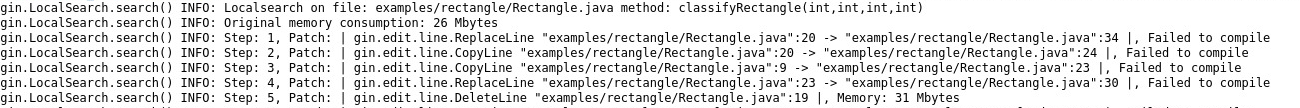
\includegraphics[width=1\textwidth]{img/Rectangle_MC_1.png}
  %\caption{Command line output: Memory Consumption Optimized %Rectangle Java program with Gin tool.}
  %\label{fig:Rectangle_MC_1}
%\end{figure}

%\vspace{1em}
%By examining the output in figure \ref{fig:Rectangle_MC_2}, we were able to identify the specific patches that led to successfully compiled code with improved memory consumption performance. Our primary objective was to identify the best patch that consumed the least memory while passing all provided tests. In summary, the optimization results indicate the best memory consumption at 14 Mbytes, representing a reduction of 46.15\%.

%\begin{figure}[htbp]
  %\centering
  %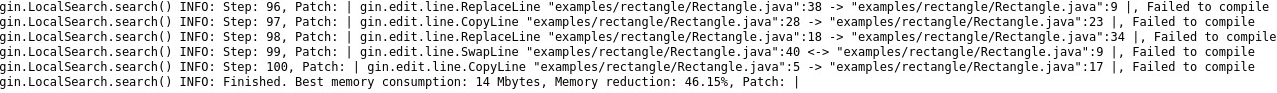
\includegraphics[width=1\textwidth]{img/Rectangle_MC_2.png}
  %\caption{Command line output: Memory Consumption Optimized Rectangle Java program with Gin tool.}
  %\label{fig:Rectangle_MC_2}
%\end{figure}

%\vspace{1em}
%Finally, in the same directory where the original Rectangle program is, the optimized code of Rectangle program for memory consumption was generated based on the best patch that consumed the lowest memory.

%\subsubsection{Multi criteria Fitness: Combined Execution time and Memory consumption}
%In our experiment, we aimed to optimize both the execution time and memory consumption together of the ‘classifyRectangle’ method in the ‘Rectangle’ Java program using Gin’s local search algorithm. As Gin’s default ‘LocalSearch’ Java class was primarily designed for execution time minimization, we adapted it to minimize both execution time and memory consumption together. The updated version of the class can be accessed at the provided \href{https://gitlabev.imtbs-tsp.eu/sticamsud/enact-internship-2023/-/blob/main/Code/gin/Version_three_ExecutionTime_and_MemoryConsumption/gin/src/main/java/gin/LocalSearch.java}{link}. The LocalSearch class has been refined to optimize both memory consumption and execution time for patches. Our experimental procedures followed the same procedures as single-criteria fitness for execution time

%\subsubsection{Experimental Results and Analysis:}

%In this section, we detail the optimization results for the "classifyRectangle" method in the Rectangle Java program, specifically focusing on execution time and memory consumption together. Using the Gin tool, the experiment showed that the method's Original execution time: 2707476462 ns and Original memory usage was 31 Mbytes, as seen in figure \ref{fig:Rectangle_EC_MC_1}.

%\begin{figure}[htbp]
  %\centering
  %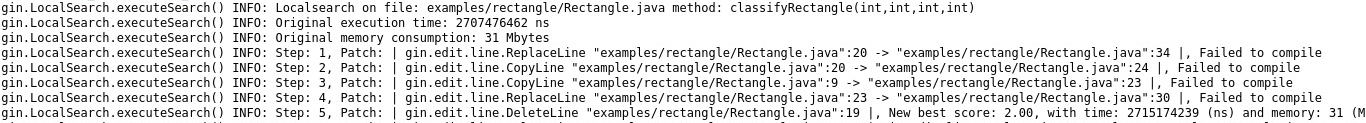
\includegraphics[width=1\textwidth]{img/Rectangle_ET_MC_1.png}
  %\caption{Command line output: Combined Execution time and Memory Consumption Optimized Rectangle Java program with Gin tool.}
  %\label{fig:Rectangle_EC_MC_1}
%\end{figure}

%By analyzing the output in figure \ref{fig:Rectangle_EC_MC_2}, we identified specific patches that resulted in a successful code compilation and enhanced both execution time and memory consumption performance. Our main goal was to find the most optimal patch one that sped up the program and consumed the least memory while still passing all the tests. In summary, the optimization results indicate the Best time: 1286266785  (ns), Speedup (\%): 52.49, Best memory consumption: 20 Mbytes, Memory reduction:35.48\%.

%\begin{figure}[htbp]
  %\centering
 % 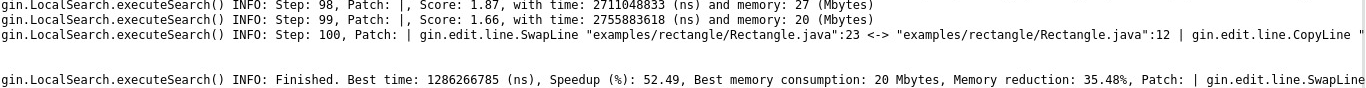
\includegraphics[width=1\textwidth]{img/Rectangle_ET_MC_2.png}
  %\caption{Command line output: Combined Execution time and Memory Consumption Optimized Rectangle Java program with Gin tool.}
 % \label{fig:Rectangle_EC_MC_2}
%\end{figure}

%\vspace{1em}
%Finally, in the same directory where the original Rectangle program is, the optimized code of Rectangle program for execution time and memory consumption together was generated. This optimization was based on the best patch, which yielded the lowest memory consumption and shortest execution time.

\vspace{-10pt}
\section{Experimental Results using JoularJX }

%\subsection{Experimental executions using JoularJX for optimised program based on the best patch given by Gin}

In the previous section, we obtained the optimization of selected programs (\ie \textit{Triangle}, \textit{GCD}, \textit{Rectangle}) using the Gin toolbox. 
%This optimization was based on single-criteria fitness (either Execution Time or Memory Consumption) and multi-criteria fitness (combining both Execution Time and Memory Consumption).  
In this section, 
%This analysis aims to 
we aim to answer our research question \textbf{RQ:2.1} (\ie \textit{Does the improvement of execution time and memory consumption reduce energy consumption?}). 

\vspace{.5em}
To do that, we first collected energy consumption measurements of the executions of the two versions, \ie original and optimised versions, of the studied programs. This was done by using \textit{JoularJX}. For this, we reused the same experimental procedures introduced in our preliminary study (\ie Section~\ref{subsec: mandelbrot java program} that details the monitoring of the energy consumed by a single program), and made modifications to the script (the \texttt{jx\_script.sh} is presented in Appendix~\ref{sec:mainscript}) to adapt it to the studied programs. 
These procedures were followed for each original and optimized version of the selected programs to monitor their energy consumption. 
%For this, we reuse and adapt the scripts used in our preliminary study (the \texttt{jx_script.sh} is presented in Appendix~\ref{sec:mainscript}). 
We then use the \texttt{Wilcoxon} statistical test to determine any significance difference of the consumed energy of the versions of the studied programs.  


%we detail our process for monitoring the energy consumption of both the original and the optimized versions of the programs using the \textit{JoulerJX} tool. We then use the \texttt{Wilcoxon} test to determine any significance difference of the consumed energy of the versions of the programs.  
%compare the energy consumption data of both versions and determine whether the optimized versions consume less energy than their original version. 
%This analysis aims to answer our research question  \textbf{RQ:2.1} (\ie \textit{Does the improvement of execution time and memory consumption reduce energy consumption?}).

\vspace{0.5em}

%After obtaining the optimized versions of the selected programs, we created two folders: one for the original versions and another for the optimized ones. In each folder, we incorporated all necessary scripts to monitor energy consumption using joularjx.
%As detailed in subsection \ref{subsec: mandelbrot java program} regarding monitoring the energy consumption of a single program, we adhered to the same experimental procedures. We made modifications to the script based on the program's name and class path. These procedures were followed for each original and optimized version of the selected programs to monitor their energy consumption. 

\vspace{0.5em}
For the energy consumption monitoring, we executed 30 times each version of each studied program using the previous script, it means that we isolated each monitoring. For instance, for evaluating the effect of the \textbf{Tactic 1}, \ie minimizing execution time, we first monitored the energy consumption of the original version of the \textit{Triangle} program. Then, we monitored the energy consumption of the optimized version for \textit{Triangle} program.
Finally, we compared collected data to evaluate if there is any significance difference between them.
We repeat the same process for the other tactic, \ie \textbf{Tactic 2} - \textit{minimizing memory consumption} and \textbf{Tactic 3} - \textit{minimizing execution time and memory consumption}, and for the others programs, \ie the \textit{GCD} and the \textit{Rectangle} programs.
%of the \textit{Triangle} program, again for a single fitness criterion: execution time.
%For each energy monitoring experiment, we ran two versions of each program: the original and the optimized version. Each version was executed for 30 iterations, consistent with the method described in subsection \ref{subsec: mandelbrot java program}. I conducted each experiment in isolation. For instance, I first monitored the energy consumption for the original Triangle program for a single fitness criterion: execution time. Subsequently, I monitored the energy consumption of the optimized Triangle program, again for a single fitness criterion: execution time.

\vspace{.5em}
Table~\ref{tab:Result} summarises the results obtained after performing our experimental study. As we can observe, 
we introduce per each version of the studied programs (see Column 1) the values obtained for each tactics applied. These obtained values correspond to the fitness values that were optimised and the corresponding energy consumption. Notice that we calculated the difference between energy consumed by the two versions of the programs (see the energy consumption values in Columns 3, 5 and 7 of the optimised versions of programs in Rows 2, 4 and 6). 
Finally, we identify the best tactic to reduce energy consumption per program (see Column 8).

%\multicolumn{5}{c}{First Video}

{\footnotesize
\begin{longtable}{|p{1.15cm}|p{1.3cm}|p{1.8cm}|p{1.5cm}|p{1.8cm}|p{1.8cm}|p{1.8cm}|p{2.5cm}|}
  \hline
  \multirow{2}{1.1cm}{\textbf{Version of Program}} 
  & \multicolumn{2}{c|}{\textbf{Tactic 1: min ET}}
  & \multicolumn{2}{c|}{\textbf{Tactic 2: min MC}} 
  & \multicolumn{2}{c|}{\textbf{Tactic 3: min ET + MC}} 
  & \multirow{2}{2.5cm}{\textbf{Best Tactic for Reducing EC}}\\
  
  \cline{2-7}
   & \textbf{ET (s)}  & \textbf{EC (J)} 
  & \textbf{MC (Mbytes)} & \textbf{EC (J)} 
  & \textbf{ET + MC} & \textbf{EC (J)} & \\
  \hline
  
%  \cline{1-7}
   Original\par Triangle & 
   1.636\kern0.5em s &
   Mean:\kern0.1em 5.834\par \vspace{.5em} [Confidence Interval:95\% (5.391,\kern0.1em 6.276)]\par \vspace{.5em} SD:\kern0.1em 1.185\vspace{.5em} Relative SD:0.203 &
   28 Mbytes &
   Mean:\kern0.1em 7.241\par \vspace{.5em} [Confidence Interval:95\% (6.968,\kern0.1em  7.514)]\par \vspace{.5em} SD:0.731\vspace{.5em} Relative SD:0.100 &
   1.773 s\par \vspace{.5em} 30 Mbytes &
   Mean:\kern0.1em 8.282\par \vspace{.5em} [Confidence Interval:95\% (7.775,\kern0.1em  8.789)]\par \vspace{.5em} SD: 1.358\vspace{.5em} Relative SD:0.164 &
   \textbf{Tactic 3}: Execution\kern0.3em time,
   Memory Consumption\par\\
   
  \cline{1-7}
  Optimised\par Triangle & 
  1.616\kern0.5em s\par \vspace{1em} Speedup: 1.22\% &
  Mean:\kern0.1em 5.023\par \vspace{.5em} [Confidence Interval:95\% (4.579,\kern0.1em 5.467)]\par \vspace{.5em} SD:\kern0.1em 1.189\par \vspace{.5em} Relative SD:0.237\vspace{.5em} \textbf{Energy consumption reduction: $\sim13.9\%$} \vspace{.5em} &
  22 Mbytes\par \vspace{.5em} Memory reduction: 21.43\% &
  Mean:\kern0.1em 6.051\par \vspace{.5em} [Confidence Interval:95\% (5.738,\kern0.1em  6.365)]\par \vspace{.5em} SD: 0.839\par \vspace{.5em} Relative SD:0.138\vspace{.5em} \textbf{Energy consumption reduction: $\sim 16.43\%$}\vspace{.5em}&
  1.751 s\par Speedup: 1.22\%.\par \vspace{.5em}
  26 Mbytes\par Memory reduction: 13.33\% &
  Mean:\kern0.1em 5.955\par \vspace{.5em} [Confidence Interval:95\% (5.697,\kern0.1em  6.212)]\par \vspace{.5em} SD: 0.689\par \vspace{.5em} Relative SD:0.116\vspace{.5em} \textbf{Energy consumption reduction: $\sim 28.11\%$}\vspace{.5em} &
  \textbf{Energy consumption reduction: $\sim 28.11\%$}
  \\
  
  \hline
%  \cline{1-7}
   Original\par GCD & 
   2.813\kern0.5em s &
   Mean:\kern0.1em27.766\par \vspace{.5em} [Confidence Interval:95\% (26.889,\kern0.1em 28.643)]\par \vspace{.5em} SD:2.349\vspace{.5em} Relative SD:0.085 &
   180 Mbytes &
   Mean:\kern0.1em26.353\par \vspace{.5em} [Confidence Interval:95\% (25.537,\kern0.1em 27.169)]\par \vspace{.5em} SD:2.186\vspace{.5em} Relative SD:0.083 &
   2.892 s\par \vspace{.5em} 158 Mbytes &
   Mean:\kern0.1em26.747\par \vspace{.5em} [Confidence Interval:95\% (25.996,\kern0.1em 27.498)]\par \vspace{.5em} SD:2.011\vspace{.5em} Relative SD:0.075 &
   \textbf{Tactic 3}: Execution\kern0.3em time,
   Memory Consumption\par\\
  
  \cline{1-7}
  Optimised\par GCD & 
  2.462\kern0.5em s\par \vspace{.5em} Speedup: 12.48\% &
  Mean:\kern0.1em13.551\par \vspace{.5em} [Confidence Interval:95\% (13.103,\kern0.1em 13.999)]\par \vspace{.5em} SD: 1.199\par \vspace{.5em} Relative SD:0.088\vspace{.5em} \textbf{Energy consumption reduction: $\sim 51.16\%$}\vspace{.5em}  &
  28 Mbytes\par \vspace{1em} Memory reduction: 84.44\% &
  Mean:\kern0.1em12.848\par \vspace{.5em} [Confidence Interval:95\% (12.406,\kern0.1em 13.290)]\par \vspace{.5em} SD:1.184\par \vspace{.5em} Relative SD:0.092\vspace{.5em} \textbf{Energy consumption reduction: $\sim 51.26\%$}\vspace{.5em} &
  2.631 s\par Speedup: 9.00\%\par \vspace{.5em}
  23 Mbytes\par Memory reduction: 85.44\% &
  Mean:\kern0.1em12.964\par \vspace{.5em} [Confidence Interval:95\% (12.554,\kern0.1em 13.375)]\par \vspace{.5em} SD:1.099\par \vspace{.5em} Relative SD:0.084\vspace{.5em} \textbf{Energy consumption reduction: $\sim 51.53\%$}\vspace{.5em} & \textbf{Energy consumption reduction: $\sim 51.53\%$}\\
  
  
  \hline
%  \cline{1-7}
   Original\par Rectangle & 
   2.629\kern0.5em s &
   Mean:\kern0.1em 6.587\par \vspace{.5em} [Confidence Interval:95\% (6.027,\kern0.1em 7.147)]\par \vspace{.5em} SD:1.499\vspace{.5em} Relative SD:0.227  &
   26 Mbytes &
   Mean:\kern0.1em 6.431\par \vspace{.5em} [Confidence Interval:95\% (5.781,\kern0.1em 7.081)]\par \vspace{.5em} SD:1.741\vspace{.5em} Relative SD:0.270 &
   2.707 s\par \vspace{.5em} 31 Mbytes &
   Mean:\kern0.1em 7.411\par \vspace{.5em} [Confidence Interval:95\% (6.926,\kern0.1em 7.895)]\par \vspace{.5em} SD:1.297\vspace{.5em} Relative SD:0.175 & 
   \textbf{Tactic 1}: Execution Time \\
   
  
  \cline{1-7}
  Optimised\par Rectangle & 
  1.213\kern0.5em s\par \vspace{.5em} Speedup: 53.86\% &
  Mean:\kern0.1em 5.217\par \vspace{.5em} [Confidence Interval:95\% (4.908,\kern0.1em 5.527)]\par \vspace{.5em} SD:0.828\par \vspace{.5em} Relative SD:0.158\vspace{.5em} \textbf{Energy consumption reduction: $\sim 20.78\%$}\vspace{.5em} &
  14 Mbytes\par \vspace{1em} Memory reduction: 46.15\% &
  Mean:\kern0.1em 5.299\par \vspace{.5em} [Confidence Interval:95\% (4.705,\kern0.1em 5.895)]\par \vspace{.5em} SD:1.594\par \vspace{.5em} Relative SD:0.300\vspace{.5em} \textbf{Energy consumption reduction: $\sim 17.6\%$}\vspace{.5em} &
  1.286 s\par Speedup: 52.59\%\par \vspace{1em}
  20 Mbytes\par Memory reduction: 35.48\% &
  Mean:\kern0.1em 6.340\par \vspace{.5em} [Confidence Interval:95\% (5.815,\kern0.1em 6.866)]\par \vspace{.5em} SD:1.407\par \vspace{.5em} Relative SD:0.221\vspace{.5em} \textbf{Energy consumption reduction: $\sim 14.45\%$}\vspace{.5em} &
  \textbf{Energy consumption reduction: $\sim 20.78\%$}
  \\
  
  
 \hline
\caption{Comparison of the energy consumed by the original vs. the optimized versions of the studied programs, \textit{where: ET=execution time in seconds, MC=memory consumption in Megabytes, EC=energy consumption in Joules}}
\label{tab:Result}
\end{longtable}
}
%Comparison between Single criteria fitness(Execution Time, Memory Consumption individually) and Multi criteria fitness(Execution Time, Memory Consumption combine).

\vspace{.5em}
In the following sections we provide the analysis of our results per program and then we discuss the results to get some general conclusions of this study.

\vspace{-5pt}
\subsection{Energy Consumption comparison for the original vs. the optimized versions of the \textit{Triangle} Program}

As we can observe in Table~\ref{tab:Result}, the Gin toolbox was able to optimised the \textit{Triangle} program by using \textbf{Tactic 1 - minimizing the execution time}. The obtained execution time was 1.636 seconds for the original version and 1.616 seconds for the optimised version, thus reducing 1.22\% of execution time (see Column 2 of Rows 1, 2) by applying Tactic 1. 
Regarding energy consumption, we obtained 5.834 joules for the original version and we obtained 5.023 joules for the optimised version. Thus, the energy consumption was reduced in 13.9\% by the optimised program (see Column 3 of Rows 1, 2) by applying Tactic 1.  
We can also observe this reduction of energy consumption in Figures~\ref{fig:triangle_tactic1_1} and~\ref{fig:triangle_tactic1_2} that shows the histogram and the box-plot of the data collected from 30 executions. Notice that the reported energy consumption are the mean values of energy consumption measurements collected from 30 executions. All of these mean values have confident error margin, \ie the relative standard deviation or coefficient of variance was lower than 5\%.


\begin{figure}
\centering
\subfigure[\textbf{Tactic 1} - Original vs. Optimized Triangle Histogram ]{
\label{fig:triangle_tactic1_1}
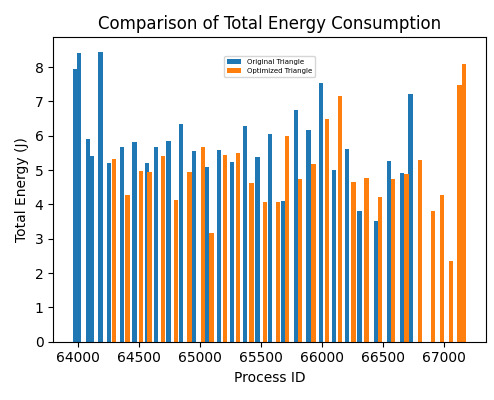
\includegraphics[width=0.45\textwidth,height=.3\textheight]{img/Triangle_ET_Comparision_histogram.png}
}
\subfigure[\textbf{Tactic 1} - Original vs. Optimized Triangle Boxplot]{
\label{fig:triangle_tactic1_2}
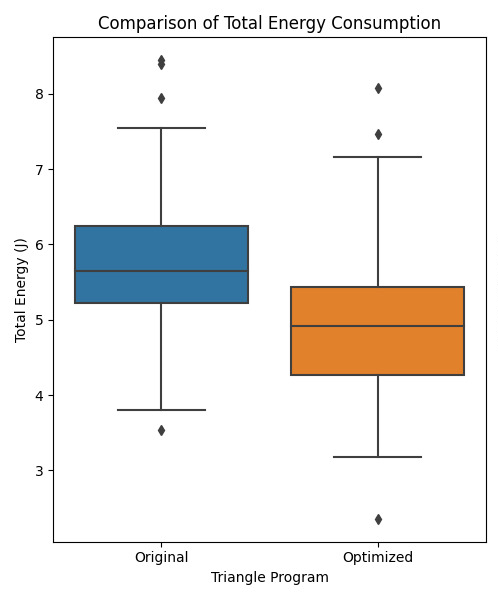
\includegraphics[width=0.47\textwidth,height=.3\textheight]{img/Triangle_ET_Comparision_boxplot.png}
}
\subfigure[\textbf{Tactic 2} - Original vs. Optimized Triangle Histogram]{
\label{fig:triangle_tactic2_1}
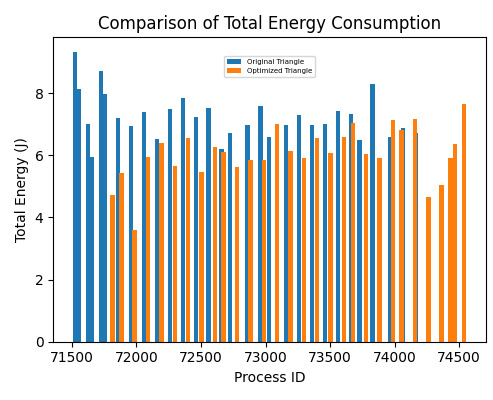
\includegraphics[width=0.45\textwidth,height=.3\textheight]{img/Triangle_MC_Comparision_histogram.png}
}
\subfigure[\textbf{Tactic 2} - Original vs. Optimized Triangle Boxplot]{
\label{fig:triangle_tactic2_2}
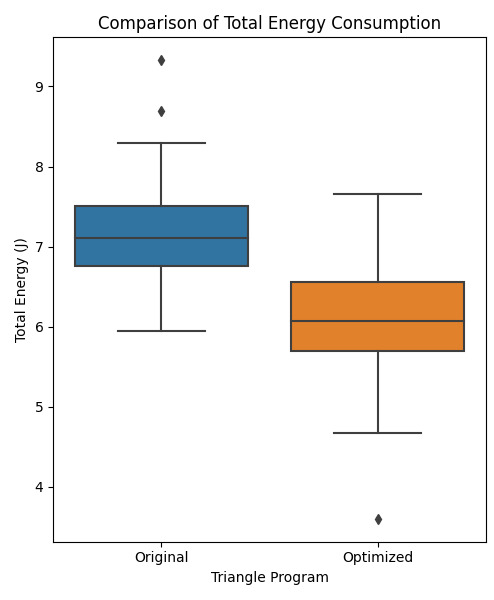
\includegraphics[width=0.47\textwidth,height=.3\textheight]{img/Triangle_MC_Comparision_boxplot.png}
}
\subfigure[\textbf{Tactic 3} - Original vs. Optimized Triangle Histogram]{
\label{fig:triangle_tactic3_1}
\includegraphics[width=0.45\textwidth,height=.3\textheight]{img/Trinagle_ET_MC_Comparison_histo.png}
} 
\subfigure[\textbf{Tactic 3} - Original vs. Optimized Triangle Boxplot]{
\label{fig:triangle_tactic3_2}
\includegraphics[width=0.47\textwidth,height=.3\textheight]{img/Trinagle_ET_MC_Comparison_box.png}
}
\caption{Energy consumption comparison for the original vs. optimized versions of the \textit{Triangle} program by applying the three studied tactics}
\label{fig:graphsTriangle}
\end{figure}

\vspace{.5em}
Moreover, the Gin toolbox was able to optimised the \textit{Triangle} program by using \textbf{Tactic 2 - minimizing the memory consumption}. The obtained memory consumption was 28 megabytes for the original version and 22 megabytes for the optimised version, thus reducing 21.43\% of memory consumption (see Column 4 of Rows 1, 2) by applying Tactic 2. 
Regarding energy consumption, we obtained 7.241 joules for the original version and we obtained 6.051 joules for the optimised version. Thus, the energy consumption was reduced in 16.43\% by the optimised program (see Column 5 of Rows 1, 2) by applying Tactic 2.
We can also observe this reduction of energy consumption in Figures~\ref{fig:triangle_tactic2_1} and~\ref{fig:triangle_tactic2_2} that shows the histogram and the box-plot of the data collected from 30 executions.

\vspace{.5em}
Finally, the Gin toolbox was able to optimised the \textit{Triangle} program by using \textbf{Tactic 3 - minimizing execution time and memory consumption}. The obtained fitness function was 1.773 seconds and 30 megabytes for the original version and 1.751 seconds and 26 megabytes for the optimised version, thus reducing 1.22\% of execution time and 13.33\% of memory consumption (see Column 6 of Rows 1, 2) by applying Tactic 3. 
Regarding energy consumption, we obtained 8.282 joules for the original version and we obtained 5.955 joules for the optimised version. Thus, the energy consumption was reduced in 28.11\% by the optimised program (see Column 7 of Rows 1, 2) by applying Tactic 3.  
We can also observe this reduction of energy consumption in Figures~\ref{fig:triangle_tactic3_1} and~\ref{fig:triangle_tactic3_2} that shows the histogram and the box-plot of the data collected from 30 executions.

\vspace{.5em}
We observe that for the \textit{Triangle} program the best tactic for reducing energy consumption was \textbf{Tactic 3 - minimizing execution time and memory consumption}. This tactic was able to reduce in 28.11\% the energy consumed by the  \textit{Triangle} program (see Column 8 of Rows 1, 2).

\vspace{.5em}
Notice that when a multi-criteria fitness function is used to optimise a code, each fitness value is optimised in a less percentage than optimising the code by using a single fitness function. For instance, while the percentage of the reduced execution time for Tactic 1 and Tactic 3 are equivalent, the percentage for the consumed memory was penalised from 21.43\% to 13.33\%. Instead of this penalisation, Tactic 3 is the most effective tactic to reduce energy consumption for the \textit{Triangle} program. It could be due to the energy consumed by programs does not only depends on execution time but also depends on the use of CPU. Therefore, if we optimise the memory consumption it could help to reduce the use of CPU, thus reducing energy consumption.

%In this subsection, we will detail the results of a comparison between two versions of the Triangle program (original and optimized) using the Wilcoxon test. Based on this analysis, we will determine which version of the Triangle program consumes more energy.  We have three optimized programs, each based on different criteria: Single criteria fitness: Execution time, Single criteria fitness: Memory consumption, Multi-criteria fitness: Combined execution time and memory consumption. For each fitness criterion, we first monitored the energy consumption of the original Triangle program, followed by its optimized version. We then compared the results using the Wilcoxon test. Because each experiment was conducted in isolation, the energy consumption of the original Triangle program varied with each fitness criterion.

\vspace{-5pt}
\subsection{Energy Consumption comparison for the original vs. the optimized versions of the \textit{Greatest Common Divisor(GCD)} Program}

As we can observe in Table~\ref{tab:Result}, the Gin toolbox was able to optimised the \textit{Greatest Common Divisor(GCD)} program by using \textbf{Tactic 1 - minimizing the execution time}. The obtained execution time was 2.813 seconds for the original version and 2.462  seconds for the optimised version, thus reducing 12.48\% of execution time (see Column 2 of Rows 3, 4) by applying Tactic 1. 
Regarding energy consumption, we obtained 27.766 joules for the original version and we obtained 13.551 joules for the optimised version. Thus, the energy consumption was reduced in 51.16\% by the optimised program (see Column 3 of Rows 3, 4) by applying Tactic 1.  
We can also observe this reduction of energy consumption in Figures~\ref{fig:gcd_tactic1_1} and~\ref{fig:gcd_tactic1_2} that shows the histogram and the box-plot of the data collected from 30 executions.
Notice that the reported energy consumption are the mean values of energy consumption measurements collected from 30 executions. All of these mean values have confident error margin, \ie the relative standard deviation or coefficient of variance was lower than 5\%.


\begin{figure}
\centering
\subfigure[\textbf{Tactic 1} - Original vs. Optimized GCD Histogram]{
\label{fig:gcd_tactic1_1}
\includegraphics[width=0.45\textwidth,height=.3\textheight]{img/GCD_ET_Comparison_his.png}
}
\subfigure[\textbf{Tactic 1} - Original vs. Optimized GCD Boxplot]{
\label{fig:gcd_tactic1_2}
\includegraphics[width=0.47\textwidth,height=.3\textheight]{img/GCD_ET_Comparison_box.png}
}
\subfigure[\textbf{Tactic 2} - Original vs. Optimized GCD Histogram]{
\label{fig:gcd_tactic2_1}
\includegraphics[width=0.45\textwidth,height=.3\textheight]{img/GCD_MC_his.png}
}
\subfigure[\textbf{Tactic 2} - Original vs. Optimized GCD Boxplot]{
\label{fig:gcd_tactic2_2}
\includegraphics[width=0.47\textwidth,height=.3\textheight]{img/GCD_MC_box.png}
}
\subfigure[\textbf{Tactic 3} - Original vs. Optimized GCD Histogram]{
\label{fig:gcd_tactic3_1}
\includegraphics[width=0.45\textwidth,height=.3\textheight]{img/GCD_ET_MC_his.png}
} 
\subfigure[\textbf{Tactic 3} - Original vs. Optimized GCD Boxplot]{
\label{fig:gcd_tactic3_2}
\includegraphics[width=0.47\textwidth,height=.3\textheight]{img/GCD_ET_MC_box.png}
}
\caption{Energy consumption comparison for the original vs. optimized versions of the \textit{Greatest Common Divisor(GCD)} program by applying the three studied tactics}
\label{fig:graphsGCD}
\end{figure}

\vspace{.5em}
Moreover, the Gin toolbox was able to optimised the \textit{Greatest Common Divisor(GCD)} program by using \textbf{Tactic 2 - minimizing the memory consumption}. The obtained memory consumption was 180 megabytes for the original version and 28 megabytes for the optimised version, thus reducing 84.44\% of memory consumption (see Column 4 of Rows 3, 4) by applying Tactic 2. Regarding energy consumption, we obtained 26.353 joules for the original version and we obtained 12.848 joules for the optimised version. Thus, the energy consumption was reduced in 51.26\% by the optimised program (see Column 5 of Rows 3, 4) by applying Tactic 2.
We can also observe this reduction of energy consumption in Figures~\ref{fig:gcd_tactic2_1} and~\ref{fig:gcd_tactic2_2} that shows the histogram and the box-plot of the data collected from 30 executions.

\vspace{.5em}
Finally, the Gin toolbox was able to optimised the \textit{Greatest Common Divisor(GCD)} program by using \textbf{Tactic 3 - minimizing execution time and memory consumption}. The obtained fitness function was 2.892 seconds and 158  megabytes for the original version and 2.631 seconds and 23 megabytes for the optimised version, thus reducing 9.00\% of execution time and 85.44\% of memory consumption (see Column 6 of Rows 3, 4) by applying Tactic 3. Regarding energy consumption, we obtained 26.747 joules for the original version and we obtained 12.964 joules for the optimised version. Thus, the energy consumption was reduced in 51.53\% by the optimised program (see Column 7 of Rows 3, 4) by applying Tactic 3. We can also observe this reduction of energy consumption in Figures~\ref{fig:gcd_tactic3_1} and~\ref{fig:gcd_tactic3_2} that shows the histogram and the box-plot of the data collected from 30 executions.

\vspace{.5em}
We observe that for the \textit{Greatest Common Divisor(GCD)} program the best tactic for reducing energy consumption was \textbf{Tactic 3 - minimizing execution time and memory consumption}. This tactic was able to reduce in 51.53\% the energy consumed by the  \textit{Greatest Common Divisor(GCD)} program (see Column 8 of Rows 3, 4).

\vspace{.5em}
Notice that when a multi-criteria fitness function is used to optimise a code, each fitness value is optimised in a less percentage than optimising the code by using a single fitness function. For instance, the percentage for the execution time was penalised from 12.48\% to 9.00\% in Tactic 1 to Tactic 3. Instead of this penalisation, Tactic 3 is the most effective tactic to reduce energy consumption for the \textit{Greatest Common Divisor(GCD)} program. It could be due to the energy consumed by programs does not only depends on execution time but also depends on the use of memory. Therefore, since Tactic 3 contains the highest memory reduce percentage it leads to reduction in energy consumption.

\vspace{-5pt}
\subsection{Energy Consumption comparison for the original vs. the optimized versions of the \textit{Rectangle} Program}

As we can observe in Table~\ref{tab:Result}, the Gin toolbox was able to optimised the \textit{Rectangle} program by using \textbf{Tactic 1 - minimizing the execution time}. The obtained execution time was 2.629 seconds for the original version and 1.213 seconds for the optimised version, thus reducing 53.86\% of execution time (see Column 2 of Rows 5, 6) by applying Tactic 1. 
Regarding energy consumption, we obtained 6.587 joules for the original version and we obtained 5.217 joules for the optimised version. Thus, the energy consumption was reduced in 20.78\% by the optimised program (see Column 3 of Rows 5, 6) by applying Tactic 1.  
We can also observe this reduction of energy consumption in Figures~\ref{fig:rectangle_tactic1_1} and~\ref{fig:rectangle_tactic1_2} that shows the histogram and the box-plot of the data collected from 30 executions.
Notice that the reported energy consumption are the mean values of energy consumption measurements collected from 30 executions. All of these mean values have confident error margin, \ie the relative standard deviation or coefficient of variance was lower than 5\%.



\begin{figure}
\centering
\subfigure[\textbf{Tactic 1} - Original vs. Optimized Rectangle Histogram]{
\label{fig:rectangle_tactic1_1}
\includegraphics[width=0.45\textwidth,height=.3\textheight]{img/Rectangle_ET_comparison_his.png}
}
\subfigure[\textbf{Tactic 1} - Original vs. Optimized Rectangle Boxplot]{
\label{fig:rectangle_tactic1_2}
\includegraphics[width=0.47\textwidth,height=.3\textheight]{img/Rectangle_ET_Compariosn_box.png}
}
\subfigure[\textbf{Tactic 2} - Original vs. Optimized Rectangle Histogram]{
\label{fig:rectangle_tactic2_1}
\includegraphics[width=0.45\textwidth,height=.3\textheight]{img/Rectangle_MC_Comparion_his.png}
}
\subfigure[\textbf{Tactic 2} - Original vs. Optimized Rectangle Boxplot]{
\label{fig:rectangle_tactic2_2}
\includegraphics[width=0.47\textwidth,height=.3\textheight]{img/Rectangle_MC_Comparion_box.png}
}
\subfigure[\textbf{Tactic 3} - Original vs. Optimized Rectangle Histogram]{
\label{fig:rectangle_tactic3_1}
\includegraphics[width=0.45\textwidth,height=.3\textheight]{img/Rectangle_ET_MC_Comparion_his.png}
} 
\subfigure[\textbf{Tactic 3} - Original vs. Optimized Rectangle Boxplot]{
\label{fig:rectangle_tactic3_2}
\includegraphics[width=0.47\textwidth,height=.3\textheight]{img/Rectangle_ET_MC_Comparion_Box.png}
}
\caption{Energy consumption comparison for the original vs. optimized versions of the \textit{Rectangle} program by applying the three studied tactics}
\label{fig:graphsRectangle}
\end{figure}

\vspace{.5em}
Moreover, the Gin toolbox was able to optimised the \textit{Rectangle} program by using \textbf{Tactic 2 - minimizing the memory consumption}. The obtained memory consumption was 26 megabytes for the original version and 14 megabytes for the optimised version, thus reducing 46.15\% of memory consumption (see Column 4 of Rows 5, 6) by applying Tactic 2. 
Regarding energy consumption, we obtained 6.431 joules for the original version and we obtained 5.299 joules for the optimised version. Thus, the energy consumption was reduced in 17.6\% by the optimised program (see Column 5 of Rows 5, 6) by applying Tactic 2.
We can also observe this reduction of energy consumption in Figures~\ref{fig:rectangle_tactic2_1} and~\ref{fig:rectangle_tactic2_2} that shows the histogram and the box-plot of the data collected from 30 executions.

\vspace{.5em}
Finally, the Gin toolbox was able to optimised the \textit{Rectangle} program by using \textbf{Tactic 3 - minimizing execution time and memory consumption}. The obtained fitness function was 2.707 seconds and 31 megabytes for the original version and 1.286 seconds and 20 megabytes for the optimised version, thus reducing 52.59\% of execution time and 35.48\% of memory consumption (see Column 6 of Rows 5, 6) by applying Tactic 3. Regarding energy consumption, we obtained 7.411 joules for the original version and we obtained 6.340 joules for the optimised version. Thus, the energy consumption was reduced in 14.45\% by the optimised program (see Column 7 of Rows 5, 6) by applying Tactic 3. We can also observe this reduction of energy consumption in Figures~\ref{fig:rectangle_tactic3_1} and~\ref{fig:rectangle_tactic3_2} that shows the histogram and the box-plot of the data collected from 30 executions.

\vspace{.5em}
We observe that for the \textit{Rectangle} program the best tactic for reducing energy consumption was \textbf{Tactic 1 - minimizing the execution time}. This tactic was able to reduce in 20.78\% the energy consumed by the  \textit{Triangle} program (see Column 8 of Rows 5, 6).

\vspace{-5pt}
\subsection{Discussion}

In Table~\ref{tab:Result}, we observe that the Gin toolbox was able to optimize the \textit{Triangle}, \textit{Greatest Common Divisor (GCD)}, and \textit{Rectangle} programs using \textbf{Tactic 1: minimizing the execution time}, \textbf{Tactic 2: minimizing memory consumption}, and \textbf{Tactic 3: minimizing execution time and memory consumption}, as discussed in Section \ref{sec:tactics}. Upon analyzing the table, we observed that the optimized version of each program consistently consumes less energy than its original version. We calculated the energy consumption reduction in percentage for each optimized version and then compared these percentages. 

\vspace{.5em}
For the \textit{Triangle} program, the energy consumption was reduced by 13.9\% with the optimized program when applying \textbf{Tactic 1} (see Column 3, Rows 1 and 2). With \textbf{Tactic 2}, the reduction was 16.43\% (see Column 5, Rows 1 and 2), and with \textbf{Tactic 3}, it was 28.11\% (see Column 7, Rows 1 and 2). We observe that, for the \textit{Triangle} program, \textbf{Tactic 3 - minimizing execution time and memory consumption} was the most effective, achieving a 28.11\% reduction in energy consumption (see Column 8, Rows 1 and 2).

\vspace{.5em}
For the \textit{Greatest Common Divisor (GCD)} program, the energy consumption was reduced by 51.16\% using the optimized program when applying \textbf{Tactic 1} (see Column 3, Rows 3 and 4). With \textbf{Tactic 2}, the reduction was 51.26\% (see Column 5, Rows 3 and 4), and with \textbf{Tactic 3}, it was 51.53\% (see Column 7, Rows 3 and 4). We observe that \textbf{Tactic 3 - minimizing execution time and memory consumption} was the most effective for the \textit{Greatest Common Divisor (GCD)} program, achieving a 51.53\% reduction in energy consumption (see Column 8, Rows 3 and 4).

\vspace{.5em}
For the \textit{Rectangle} program, the energy consumption was reduced by 20.78\% using the optimized program when applying \textbf{Tactic 1} (see Column 3, Rows 5 and 6). With \textbf{Tactic 2}, the reduction was 17.6\% (see Column 5, Rows 5 and 6), and with \textbf{Tactic 3}, it was 14.45\% (see Column 7, Rows 5 and 6). We observe that, for the \textit{Rectangle} program, \textbf{Tactic 1 - minimizing the execution time} was the most effective, achieving a 20.78\% reduction in energy consumption (see Column 8, Rows 5 and 6).

\vspace{.5em}
To definitively determine which tactic yields the highest energy consumption reduction, further experiments are needed. However, based on our current results, we can conclude that the optimized versions program using the "gin" tool, across all three tactics, consistently consume less energy than their original version program. This evidence supports a positive answer to research question \textbf{RQ2.1}: improvements in the execution time and memory consumption of programs do indeed lead to reduced energy consumption.

\chapter{Conclusion and Next Steps}\label{ch:conclusion}
\section{Conclusion}
In our internship, the main objective was to investigate tactics for enhancing software energy efficiency. From this objective, we formulated two research questions: 
\vspace{-6pt}
\begin{itemize}
    \item \textbf{RQ1:} Which tactics improve energy efficiency?
    \vspace{-8pt}
    \item \textbf{RQ2:} How can we automate the integration of these tactics to minimize energy consumption?
\end{itemize}
\vspace{-5pt}
In response to Research Question 1 (\textbf{RQ1}), we delved into various tactics such as Architectural Tactics, Design Patterns, and Code Refactoring. Through a comparative analysis, we discerned the benefits and drawbacks of each tactic. Code refactoring emerged as particularly versatile across various software types. We not only identified these tactics but also detailed insights into their implementation, emphasizing practical methods to embed them in software. Monitoring energy consumption was essential for our research. Among the considered software tools for energy consumption profiling, JoularJX was the most fitting for our focus on Java-based software. This preference stemmed from JoularJX's ability to offer real-time monitoring at the source code level, functioning as a Java agent. %It delivered precise power and energy measurements for both GNU/Linux and Windows platforms, aligning perfectly with our emphasis on Java-based software. 
To automate the monitoring process using the JoularJX tool, we developed two bash scripts tailored to its updated 2.0 version. %Within these scripts were several Python files, like \texttt{jx\_gatherData.py}, \texttt{jx\_plot.py}, \texttt{jx\_process\_level\_methods.py}, \texttt{shapiro\_wilk\_test\_energy.py}. Our scripts would create directories for result organization, execute the Java program or project for 30 iterations with the JoularJX agent attached, and collect energy and power data. Subsequent processing and analysis were done using the Python scripts. The \texttt{jx\_plot.py} generated visual representations from the data, while the Shapiro-Wilk tests ascertained normality in the energy and power datasets.
Another intern, \texttt{Lyne Gabriella NENGUEKO NOUMBISSIE}, utilized these scripts in her research, \texttt{Evaluation of energy-efficiency requirements through a systematic test case
generation.}

\vspace{.5em}
In \textbf{RQ2}, we focused on the automation of integrating tactics to reduce energy consumption. This approach utilized genetic improvement, and as part of our research, we introduced a tool called GIN. Under research question \textbf{RQ2}, three sub-questions were identified:
\vspace{-5pt}
\begin{itemize}
    \item \textbf{RQ2.1}: Does the improvement of execution time and memory consumption reduce energy consumption?
    \vspace{-8pt}
    \item \textbf{RQ2.2}: Could code refactoring integrate into GI? Which elements need to be extended in the Gin tool?
    \vspace{-8pt}
    \item \textbf{RQ2.3}: In which extent code refactoring genetically improve the software to reduce energy consumption?
\end{itemize}
\vspace{-5pt}
Analysis of the results from Table~\ref{tab:Result} reveals that the Gin toolbox effectively optimized the \textit{Triangle}, \textit{GCD}, and \textit{Rectangle} programs across three tactics (Section \ref{sec:tactics}). Across these programs, the optimized versions consistently used less energy than their originals. For the \textit{Triangle} program, the most energy savings (28.11\%) was achieved with \textbf{Tactic 3}. For the \textit{GCD} program, energy consumption was most reduced (51.53\%) also by \textbf{Tactic 3}. However, for the \textit{Rectangle} program, the most reduction (20.78\%) was observed with \textbf{Tactic 1}. To definitively determine which tactic yields the highest energy consumption reduction, further experiments are needed. However, based on our current results, we can conclude that the optimized versions program using the "gin" tool, across all three tactics, consistently consume less energy than their original version program. This evidence supports a positive answer to research question \textbf{RQ2.1}: improvements in the execution time and memory consumption of programs do indeed lead to reduced energy consumption.

\vspace{.5em}
A comprehensive literature review was conducted, and it was observed that while various code refactoring techniques could improve software performance, their impact on energy efficiency varied based on the software's specific context. Notably, techniques like 'Convert Local Variable to Field', 'Introduce Parameter Object', and others showed promise in reducing energy consumption. The Genetic Improvement (GIN) tool, which leveraged Genetic Programming for software enhancement, presented an ideal platform for integrating these techniques. The \texttt{StatementEdit} class within GIN appeared to be the most fitting for this integration, paving the way for potentially higher software quality and energy efficiency. This study effectively addressed the research question, highlighting the potential synergies between refactoring techniques and the GIN tool. Based on this analysis, research question \textbf{RQ2.2} was answered: Code refactoring techniques could indeed be integrated into the Genetic Improvement tool, Gin. For this integration, the \texttt{StatementEdit} class in Gin needed to be extended.

\vspace{.5em}
Due to time constraints, we were unable to address our research question \textbf{RQ2.3}. However, we provide detailed information in the following section, Section \ref{sec:nextSteps}, on how the corresponding experiment can be conducted.

\vspace{.5em}
It is very important to make software developers aware of the negative effects of energy consumption. This internship helped me to learn a lot of new things about energy efficiency in the software domain. I am sure that this knowledge will help me a lot in the future. This work made me aware of how important is to reduce energy consumption at the software level and how much energy we can save by using energy-friendly programs or software.








\section{Next steps}\label{sec:nextSteps}
%\section{Future Work}

In response to \textbf{RQ2.3}, our next steps will involve integrating the selected code refactoring techniques such as \texttt{Convert Local Variable to Field}, \texttt{Introduce Parameter Object}, and \texttt{Move Method} into the identified \texttt{StatementEdit} class within Gin. Before this integration, we need to integrate code smell detection technique in the Gin tool. This will allow us for efficient detection and tracing of code smells. 

\vspace{.5em}
Our first step is to identify if there are any code smells present. Only upon detecting code smells can we then integrate the selected code refactoring techniques. Under this step, we have two sub-steps. The first is to translate the code into Abstract Syntax Tree (AST) format. The second sub-step is to identify the tool that detects code smells from the code in Abstract Syntax Tree (AST) format using specific code smell detection technique. Once identified, the techniques used by the identified code smell detection tool will be integrated into the 'Gin' tool for detecting code smells.

\vspace{.5em}
\cite{liu2017detection} presents famous code smeel detection tools: \texttt{Checkstyle}, \texttt{JDeodorant}. These two tool detect code smells from the code in Abstract Syntax Tree (AST) format using specific code smell detection technique. \texttt{Checkstyle} is a well-known static code analysis tool, it can detect 4 code smells Large Class, Long Method, Long Parameter List, and Duplicated Code.\texttt{JDeodorant} is an Eclipse plug-in\cite{DBLP:conf/wcre/TsantalisCC18}. It can automatically detect 4 code smells Feature Envy, God Class, Long Method, and Switch Statement. It can achieve high detection accuracy. In addition, JDeodorant can achieve a good visualization of detection results. But at present it only can detect 4 code smells. \texttt{Checkstyle} uses a metric-based approach to detect code smells, where it checks the source code for violations of specified metrics such as cyclomatic complexity, lines of code, and number of parameters\cite{DBLP:journals/ese/FontanaMZM16}. It was not mentioned specifically what approach used in the JDeodorant code smell detection tool.

\vspace{.5em}
\cite{DBLP:journals/corr/abs-2012-08842} presents an up-to-date review of state-of-the-art techniques and tools used for code smell detection and visualization. The study found that the most commonly used approaches for code smell detection are search-based (30.1\%), metric-based (24.1\%), and symptom-based (19.3\%). The study does offer insights into the strengths and limitations of various approaches, which can guide us in deciding the most suitable technique for our specific needs. For instance, search-based approaches are effective in detecting code smells. The effectiveness of a given technique could depend on factors like the specific codebase under analysis, the programming language in use, and the desired accuracy and precision for detecting code smells.

\vspace{.5em}
We have selected the search-based code smell detection technique for integration into the Gin tool. Search-based code smell detection is a technique that uses search algorithms to identify instances of code smells in software systems. To integrate search-based code smell detection into GIN, we would need to modify the Gin tool’s source code to incorporate the desired search-based technique. This would likely involve implementing the search algorithm and defining a fitness function that evaluates candidate solutions based on their ability to detect code smells. We may also need to modify GIN’s existing genetic operators (e.g., mutation and crossover) to work with the new search-based approach.

\vspace{.5em}
After integrating code smell detection techniques into the GIN tool, we can proceed to incorporate code refactoring techniques. Once these are integrated, we will conduct experiments using the extended version of the GIN tool to determine whether the optimized version of the program or project results in energy savings in the software domain thereby addressing Research Question \textbf{RQ2.3}.


% Start the appendix environment
\begin{appendices}

\chapter{Experimental artifacts}
%\section{Energy consumption monitoring of mandelbrot program using JoularJX}
\section{The \texttt{jx\_script.sh} script}\label{sec:mainscript}

\begin{lstlisting}
#!/bin/bash

if [ "$#" -ne 1 ];then
    echo "Un unique argument est attendu : le nom du programme (sans l'extension)" >&2
    exit 1
fi

programme=$1
jar="/opt/joularjx/joularjx-2.0.jar"
mkdir "jx_results"
mkdir "jx_results/energy"
mkdir "jx_results/energy/methods"
mkdir "jx_results/energy/calltrees"
mkdir "jx_results/energy_filtered"
mkdir "jx_results/energy_filtered/methods"
mkdir "jx_results/energy_filtered/calltrees"
mkdir "jx_results/power"
mkdir "jx_results/power/methods"
mkdir "jx_results/power/calltrees"
mkdir "jx_results/power_filtered"
mkdir "jx_results/power_filtered/methods"
mkdir "jx_results/power_filtered/calltrees"

mkdir "mandelbrot_bitmap"

for param in 15000 20000 30000 40000 # Nombre d'élements dans un tableau
do    
    #for i in 1 2  # Nombre d'itérations
    for i in {1..30}  # Nombre d'itérations
    do 
	echo "running java  with parameter $param, iteration $i"
	# Nous avons besoin du pid du processus java pour pouvoir correctement gérer les fichiers créés par JoularJX
	if [ $i == 1 ];then
	    # On sauvegarde les pmb pour la première itération
	    java -javaagent:$jar $programme $param > "mandelbrot_bitmap/java_temp.pmb" &
	else
	    java -javaagent:$jar $programme $param > /dev/null 2>/dev/null &
	fi
	java_pid=$!
	wait $!

	# Sauvegarde du pmb
	if [ -e "mandelbrot_bitmap/java_temp.pmb" ];then
	    tail -n+6 "mandelbrot_bitmap/java_temp.pmb" > "mandelbrot_bitmap/java_$param.pmb"
	    rm -f "mandelbrot_bitmap/java_temp.pmb"
	fi
	
	fichier_energy_methods="joularJX-"$java_pid"-all-methods-energy.csv"
	fichier_energy_calltrees="joularJX-"$java_pid"-all-call-trees-energy.csv"
	fichier_energy_filtered_methods="joularJX-"$java_pid"-filtered-methods-energy.csv"
	fichier_energy_filtered_calltrees="joularJX-"$java_pid"-filtered-call-trees-energy.csv"
	fichier_power_methods="joularJX-"$java_pid"-all-methods-power.csv"
	fichier_power_calltrees="joularJX-"$java_pid"-all-call-trees-power.csv"
	fichier_power_filtered_methods="joularJX-"$java_pid"-filtered-methods-power.csv"
	fichier_power_filtered_calltrees="joularJX-"$java_pid"-filtered-call-trees-power.csv"

	# Tri des fichiers vides
	find . -name "$fichier_energy_methods" -type f -print0 | while IFS= read -r -d '' f
	do
	    if [ -s "$f" ]; then
		# Non-empty file
		mv "$f" "jx_results/energy/methods"
		#echo "Moved $f to jx_results/energy/methods"
	    else
		# Empty file
		#echo "Deleting empty file: $f"
		rm -f "$f"
	    fi
	done
	find . -name "$fichier_energy_calltrees" -type f -print0 | while IFS= read -r -d '' f
	do
	    if [ -s "$f" ]; then
		# Non-empty file
		mv "$f" "jx_results/energy/calltrees"
		#echo "Moved $f to jx_results/energy/calltrees"
	    else
		# Empty file
		#echo "Deleting empty file: $f"
		rm -f "$f"
	    fi
	done
	find . -name "$fichier_energy_filtered_methods" -type f -print0 | while IFS= read -r -d '' f
	do
	    if [ -s "$f" ]; then
		# Non-empty file
		mv "$f" "jx_results/energy_filtered/methods"
		#echo "Moved $f to jx_results/energy_filtered/methods"
	    else
		# Empty file
		#echo "Deleting empty file: $f"
		rm -f "$f"
	    fi
	done
	find . -name "$fichier_energy_filtered_calltrees" -type f -print0 | while IFS= read -r -d '' f
	do
	    if [ -s "$f" ]; then
		# Non-empty file
		mv "$f" "jx_results/energy_filtered/calltrees"
		#echo "Moved $f to jx_results/energy_filtered/calltrees"
	    else
		# Empty file
		#echo "Deleting empty file: $f"
		rm -f "$f"
	    fi
	done
	find . -name "$fichier_power_methods" -type f -print0 | while IFS= read -r -d '' f
	do
	    if [ -s "$f" ]; then
		# Non-empty file
		mv "$f" "jx_results/power/methods"
		#echo "Moved $f to jx_results/power/methods"
	    else
		# Empty file
		#echo "Deleting empty file: $f"
		rm -f "$f"
	    fi
	done
	find . -name "$fichier_power_calltrees" -type f -print0 | while IFS= read -r -d '' f
	do
	    if [ -s "$f" ]; then
		# Non-empty file
		mv "$f" "jx_results/power/calltrees"
		#echo "Moved $f to jx_results/power/calltrees"
	    else
		# Empty file
		#echo "Deleting empty file: $f"
		rm -f "$f"
	    fi
	done
	find . -name "$fichier_power_filtered_methods" -type f -print0 | while IFS= read -r -d '' f
	do
	    if [ -s "$f" ]; then
		# Non-empty file
		mv "$f" "jx_results/power_filtered/methods"
		#echo "Moved $f to jx_results/power_filtered/methods"
	    else
		# Empty file
		#echo "Deleting empty file: $f"
		rm -f "$f"
	    fi
	done
	
	find . -name "$fichier_power_filtered_calltrees" -type f -print0 | while IFS= read -r -d '' f
	do
	    if [ -s "$f" ]; then
		# Non-empty file
		mv "$f" "jx_results/power_filtered/calltrees"
		#echo "Moved $f to jx_results/power_filtered/calltrees"
	    else
		# Empty file
		#echo "Deleting empty file: $f"
		rm -f "$f"
	    fi
	done
    done
done

# used to gather power and engery consumption data using JoularJX and save it t CSV file.
python3 jx_gatherData.py "jx_results/"

#used to analyze the power consumption data at the method level, i.e., it breaks down the data into individual methods and calculates the energy and power consumed by each method.
python3 jx_process_level_methods.py "jx_results/"

# used to generate graphs from the power and engery consumption data saved in the CSV file generated by jx_gatherData.py.
python3 jx_plot.py  "jx_graphs"

# for box plotting the total energy for all the process id
python3 jx_plot_geom_boxplot.py

#used to perform a Shapiro-Wilk test on the energy consumption data to check for normality.
python3 shapiro_wilk_test_energy.py

#used to perform a Shapiro-Wilk test on the power consumption data to check for normality.
python3 shapiro_wilk_test_power.py
\end{lstlisting}

%In this experiment, we monitored the energy consumption of a single Java program, mandelbrot.java using JoularJX. We used JoularJX 2.0 version to obtain updated tree structure results in the output directory. To execute the Java program with JoularJX, we prepared a bash script named "jx\_script.sh", which includes several Python files: "jx\_gatherData.py," "jx\_plot.py," "jx\_process\_level\_methods.py," "shapiro\_wilk\_test\_energy.py," and "shapiro\_wilk\_test\_power.py.". Now, we will explain how the script works to collect the data of energy consumption of the program (mandelbrot.java).\par

%The script began by checking if a single argument, which was expected to be the name of the program without the file extension, was provided. If not, an error message was displayed. Then, a series of directories were created to organize the results. These directories included "jx\_results" as the main folder, which contained subfolders for "energy", "energy\_filtered", "power", and "power\_filtered". Each of these subfolders further contained "methods" and "calltrees" directories.\par

%Next, the script created a directory named "mandelbrot\_bitmap". The script then entered a loop where it ran the Java program with different parameters (15000, 20000, 30000, and 40000) for a certain number of iterations (30 in this case). The program was run with the JoularJX agent attached, which collected energy and power consumption data. For the first iteration, the program's output was saved as "mandelbrot\_bitmap/java\_temp.pmb".\par

%After each execution, four types of files were created by JoularJX, representing energy and power data at different levels of granularity. These files had specific names based on the process ID of the Java program. The script then moved the non-empty files to their respective directories under "jx\_results". If a file was empty, it was deleted.\par

%Once the iterations were completed, the script proceeded to execute Python scripts for further data processing and analysis. The script "jx\_gatherData.py" read energy and power data from CSV files in specific directories and created Pandas dataframes to store the data. The dataframes were then processed to extract relevant information (such as method names, parameters, iterations, and energy/power consumption), and this information was stored in lists. The lists were then used to create new dataframes with meaningful column names, which were then saved to CSV files. After that,  the "jx\_process\_level\_methods.py" script read data from a CSV file containing energy and power consumption values for different iterations of a process. It then calculated the total and average energy consumption, and total and average power consumption for each iteration, and wrote these results to a new CSV file. The code used the Python CSV module to read and write CSV files and stored the results in dictionaries. The "jx\_process\_level\_methods.py" script analyzed the power consumption data at the method level, calculating energy and power for each method. The "jx\_plot.py" script generated graphs based on the gathered data. Subsequently, the "jx\_plot\_geom\_boxplot.py" script created box plots to visualize the total energy consumption across all process IDs. 

%Lastly, the script ran the "shapiro\_wilk\_test\_energy.py" and "shapiro\_wilk\_test\_power.py" scripts, which performed Shapiro\-Wilk tests to check for normality in the energy and power consumption data, respectively.\par

%\subsubsection{Experimental Procedure:} To execute the experiment, perform the following steps:

%\begin{enumerate}
%\item \textbf{Clone the Repository:} Start by cloning the repository using the following command:

%\begin{verbatim}
%git clone https://gitlabev.imtbs-tsp.eu/sticamsud/enact-internship-2023.git
%\end{verbatim}

%\item \textbf{Navigate to the Project Directory:} Change the directory to the project folder:
%\begin{verbatim}
%cd enact-internship-2023/Code/Prem_Experiment
%\end{verbatim}

%\item \textbf{Install JoularJX:} Follow the instructions provided on the JoularJX website to install the JoularJX. Visit: \url{https://github.com/joular/joularjx}

%\item \textbf{Compile the Java Program:} Compile the mandelbrot.java program by running the following command:
%\begin{verbatim}
%javac mandelbrot.java
%\end{verbatim}

%\item \textbf{Execute the Script:} Run the script by entering the following %command:
%\begin{verbatim}
%./jx_script.sh mandelbrot
%\end{verbatim}

%\end{enumerate}

%\section{Energy consumption monitoring of cMath\_original project using JoularJX:}

%In the second experiment, the energy consumption of a project called 'cMath\_original' was monitored using JoularJX. Similar to the previous experiment, JoularJX version 2.0 was used to obtain updated tree structure results in the output directory. To execute all test cases of the project together, a new test class named 'RunAllSuite.java' was created in the test directory. To execute the 'RunAllSuite.java' class with JoularJX, it was necessary to download the \href{http://www.java2s.com/Code/Jar/c/Downloadcpsuite126jar.htm}{cpsuite-1.2.6.jar.zip} file and unzip it. A script called 'jx\_script\_math.sh' in the 'cMath\_original' directory was used to execute the 'RunAllSuite.java' class, which captured power and energy measurements using the JoularJX and managed the resulting files. The script included several Python files: "jx\_gatherData.py," "jx\_plot.py," "jx\_process\_level\_methods.py," "shapiro\_wilk\_test\_energy.py," and "shapiro\_wilk\_test\_power.py." 

%The script set up directories for storing output files. These directories included "jx\_results" as the main folder, which contained subfolders for "energy", "energy\_filtered", "power", and "power\_filtered". Each of these subfolders further contained "methods" and "calltrees" directories.

%The script set the Java classpath and ran the 'RunAllSuite.java' program in a loop for 30 iterations. During the first iteration, the output was saved to a file named 'java\_temp.pmb,' and for subsequent iterations, the output was discarded. After each execution, four types of files were created by JoularJX, representing energy and power data at different levels of granularity. These files had specific names based on the process ID of the Java program. The script then moved the non-empty files to their respective directories under "jx\_results". If a file was empty, it was deleted.

%Once the iterations were completed, the script proceeded to execute Python scripts for further data processing and analysis. The script "jx\_gatherData.py" read energy and power data from CSV files in specific directories and created Pandas data frames to store the data. The data frames were then processed to extract relevant information (such as method names, parameters, iterations, and energy/power consumption), and this information was stored in lists. The lists were then used to create new data frames with meaningful column names, which were then saved to CSV files. After that, the "jx\_process\_level\_methods.py" script read data from a CSV file containing energy and power consumption values for different iterations of a process. It then calculated the total and average energy consumption, and total and average power consumption for each process id, and wrote these results to a new CSV file. The code used the Python CSV module to read and write CSV files and stored the results in dictionaries. The "jx\_process\_level\_methods.py" script analyzed the power consumption data at the method level, calculating energy and power for each method. The "jx\_plot.py" script generated graphs based on the gathered data. Subsequently, the "jx\_plot\_geom\_boxplot.py" script created box plots to visualize the total energy consumption across all process IDs.

%Lastly, the script ran the "shapiro\_wilk\_test\_energy.py" and "shapiro\_wilk\_test\_power.py" scripts, which performed Shapiro\-Wilk tests to check for normality in the energy and power consumption data, respectively.\par


%\subsubsection{Experimental Procedure:} To execute the experiment, perform the following steps:

%\begin{enumerate}
%\item \textbf{Clone the Repository:} Start by cloning the repository using the following command:

%\begin{verbatim}
%git clone https://gitlabev.imtbs-tsp.eu/sticamsud/enact-internship-2023.git
%\end{verbatim}

%\item \textbf{Navigate to the Project Directory:} Change the directory to the project folder:
%\begin{verbatim}
%cd enact-internship-2023/Code/Prem_Experiment/cMath_original
%\end{verbatim}

%\item \textbf{Install JoularJX:} Follow the instructions provided on the JoularJX website to install the JoularJX. Visit: \url{https://github.com/joular/joularjx}

%\item \textbf{Navigate to the RunAllSuite.java file:}
%\begin{verbatim}
%cd src/test/java
%\end{verbatim}

%\item \textbf{Compile the RunAllSuite.java file:} Compile the RunAllSuite.java program by running the following command:
%\begin{verbatim}
%javac -cp /home/tareq/cpsuite-1.2.6.jar:/usr/share/java/junit4.jar RunAllSuite.java
%\end{verbatim}

%\item \textbf{Move the compiled file(RunAllSuite.class) in the bin folder:} Move the compiled file
%(RunAllSuite.class) in the bin folder by running the following command
%\begin{verbatim}
%cd ../../../../../
%cd Prem_Experiment/cMath_original/bin
%\end{verbatim}

%\item \textbf{Execute the Script:} Run the script by entering the following command:
%\begin{verbatim}
%cd ../
%./jx_script_math.sh 
%\end{verbatim}

%\end{enumerate}

\section{The \texttt{RunAllSuite} java code}\label{sec:alltests}

\begin{lstlisting}
import org.junit.extensions.cpsuite.ClasspathSuite;
import org.junit.extensions.cpsuite.ClasspathSuite.*;
import org.junit.internal.TextListener;
import org.junit.runner.RunWith;
import org.junit.runner.JUnitCore;
import static org.junit.extensions.cpsuite.SuiteType.*;

@RunWith(ClasspathSuite.class)
@SuiteTypes({ JUNIT38_TEST_CLASSES, TEST_CLASSES })
public class RunAllSuite {
        public static void main(String args[]) {
        	JUnitCore junit = new JUnitCore();
            junit.addListener(new TextListener(System.out));
            junit.run(RunAllSuite.class);
        }
}
\end{lstlisting}

\section{The \texttt{LocalSearch} java code for Tactic 2: Minimize Memory Consumption}\label{sec:LocalSearch_Memory}

\begin{lstlisting}
package gin;

import com.sampullara.cli.Args;
import com.sampullara.cli.Argument;
import gin.edit.Edit;
import gin.edit.Edit.EditType;
import gin.test.InternalTestRunner;
import gin.test.UnitTestResult;
import gin.test.UnitTestResultSet;
import org.apache.commons.io.FilenameUtils;
import org.apache.commons.rng.simple.JDKRandomBridge;
import org.apache.commons.rng.simple.RandomSource;
import org.pmw.tinylog.Logger;

import java.io.File;
import java.io.Serial;
import java.io.Serializable;
import java.util.Collections;
import java.util.List;
import java.util.Random;

/**
 * Simple local search. Takes a source filename and a method signature, optimizes it.
 * Assumes the existence of accompanying Test Class.
 * The class must be in the top level package if classPath not provided.
 */
public class LocalSearch implements Serializable {

    @Serial
    private static final long serialVersionUID = -92020344633720482L;

    private static final int WARMUP_REPS = 10;

    @Argument(alias = "f", description = "Required: Source filename", required = true)
    protected File filename = null;

    @Argument(alias = "m", description = "Required: Method signature including arguments." +
            "For example, \"classifyTriangle(int,int,int)\"", required = true)
    protected String methodSignature = "";

    @Argument(alias = "s", description = "Seed")
    protected Integer seed = 123;

    @Argument(alias = "n", description = "Number of steps")
    protected Integer numSteps = 100;

    @Argument(alias = "d", description = "Top directory")
    protected File packageDir;

    @Argument(alias = "c", description = "Class name")
    protected String className;

    @Argument(alias = "cp", description = "Classpath")
    protected String classPath;

    @Argument(alias = "t", description = "Test class name")
    protected String testClassName;

    @Argument(alias = "et", description = "Edit type: this can be a member of the EditType enum (LINE,STATEMENT,MATCHED_STATEMENT,MODIFY_STATEMENT); the fully qualified name of a class that extends gin.edit.Edit, or a comma-separated list of both")
    protected String editType = EditType.LINE.toString();

    /**
     * allowed edit types for sampling: parsed from editType
     */
    protected List<Class<? extends Edit>> editTypes;

    @Argument(alias = "ff", description = "Fail fast. "
            + "If set to true, the tests will stop at the first failure and the next patch will be executed. "
            + "You probably don't want to set this to true for Automatic Program Repair.")
    protected Boolean failFast = false;

    protected SourceFile sourceFile;
    protected Random rng;
    InternalTestRunner testRunner;

    // Constructor parses arguments
    LocalSearch(String[] args) {
        Args.parseOrExit(this, args);
        editTypes = Edit.parseEditClassesFromString(editType);

        this.sourceFile = SourceFile.makeSourceFileForEditTypes(editTypes, this.filename.toString(), Collections.singletonList(this.methodSignature));

        this.rng = new JDKRandomBridge(RandomSource.MT, Long.valueOf(seed));
        if (this.packageDir == null) {
            this.packageDir = (this.filename.getParentFile() != null) ? this.filename.getParentFile().getAbsoluteFile() : new File(System.getProperty("user.dir"));
        }
        if (this.classPath == null) {
            this.classPath = this.packageDir.getAbsolutePath();
        }
        if (this.className == null) {
            this.className = FilenameUtils.removeExtension(this.filename.getName());
        }
        if (this.testClassName == null) {
            this.testClassName = this.className + "Test";
        }
        this.testRunner = new InternalTestRunner(className, classPath, testClassName, failFast);
    }

    // Instantiate a class and call search
    public static void main(String[] args) {
        LocalSearch simpleLocalSearch = new LocalSearch(args);
        simpleLocalSearch.search();
    }

    // Apply empty patch and return memory consumption
    private long memoryOriginalCode() {
        Patch emptyPatch = new Patch(this.sourceFile);
        UnitTestResultSet resultSet = testRunner.runTests(emptyPatch, WARMUP_REPS);

        if (!resultSet.allTestsSuccessful()) {
            if (!resultSet.getCleanCompile()) {
                Logger.error("Original code failed to compile");
            } else {
                Logger.error("Original code failed to pass unit tests");
                for (UnitTestResult testResult : resultSet.getResults()) {
                    Logger.error(testResult);
                }
            }
            System.exit(0);
        }

        return resultSet.totalMemoryUsage() / WARMUP_REPS;
    }

    // Simple local search
    private void search() {
        Logger.info(String.format("Localsearch on file: %s method: %s", filename, methodSignature));

        // Memory consumption of original code
        long origMemory = memoryOriginalCode();
        Logger.info("Original memory consumption: " + origMemory + " Mbytes");

        // Start with empty patch
        Patch bestPatch = new Patch(this.sourceFile);
        long bestMemory = origMemory;

        for (int step = 1; step <= numSteps; step++) {
            Patch neighbour = neighbour(bestPatch);
            UnitTestResultSet testResultSet = testRunner.runTests(neighbour, 1);

            String msg;

            if (!testResultSet.getValidPatch()) {
                msg = "Patch invalid";
            } else if (!testResultSet.getCleanCompile()) {
                msg = "Failed to compile";
            } else if (!testResultSet.allTestsSuccessful()) {
                msg = "Failed to pass all tests";
            } else if (testResultSet.totalMemoryUsage() >= bestMemory) {
                msg = "Memory: " + testResultSet.totalMemoryUsage() + " Mbytes";
            } else {
                bestPatch = neighbour;
                bestMemory = testResultSet.totalMemoryUsage();
                msg = "New best memory consumption: " + bestMemory + " Mbytes ";
            }

            Logger.info(String.format("Step: %d, Patch: %s, %s ", step, neighbour, msg));
        }

        Logger.info(String.format("Finished. Best memory consumption: %d Mbytes, Memory reduction: %.2f%%, Patch: %s",
                bestMemory,
                100.0 * ((origMemory - bestMemory) / (1.0 * origMemory)),
                bestPatch));

        bestPatch.writePatchedSourceToFile(sourceFile.getRelativePathToWorkingDir() + ".optimised");
    }

    /**
     * Generate a neighboring patch, either by deleting an edit or adding a new one.
     *
     * @param patch Generate a neighbor of this patch.
     * @return A neighboring patch.
     */
    Patch neighbour(Patch patch) {
        Patch neighbour = patch.clone();

        if (neighbour.size() > 0 && rng.nextFloat() > 0.5) {
            neighbour.remove(rng.nextInt(neighbour.size()));
        } else {
            neighbour.addRandomEditOfClasses(rng, editTypes);
        }

        return neighbour;
    }
}

\end{lstlisting}


\section{The \texttt{LocalSearch} java code for Tactic 3: Minimising Execution Time and minimising Memory Consumption together}\label{sec:LocalSearch_Time_Memory}

\begin{lstlisting}
package gin;

import com.sampullara.cli.Args;
import com.sampullara.cli.Argument;
import gin.edit.Edit;
import gin.edit.Edit.EditType;
import gin.test.InternalTestRunner;
import gin.test.UnitTestResult;
import gin.test.UnitTestResultSet;
import org.apache.commons.io.FilenameUtils;
import org.apache.commons.rng.simple.JDKRandomBridge;
import org.apache.commons.rng.simple.RandomSource;
import org.pmw.tinylog.Logger;

import java.io.File;
import java.io.Serial;
import java.io.Serializable;
import java.util.Collections;
import java.util.List;
import java.util.Random;
import java.util.Scanner;

public class LocalSearch implements Serializable {

    @Serial
    private static final long serialVersionUID = -92020344633720482L;

    private static final int WARMUP_REPS = 10;

    @Argument(alias = "f", description = "Required: Source filename", required = true)
    protected File filename = null;

    @Argument(alias = "m", description = "Required: Method signature including arguments." +
            "For example, \"classifyTriangle(int,int,int)\"", required = true)
    protected String methodSignature = "";

    @Argument(alias = "s", description = "Seed")
    protected Integer seed = 123;

    @Argument(alias = "n", description = "Number of steps")
    protected Integer numSteps = 100;

    @Argument(alias = "d", description = "Top directory")
    protected File packageDir;

    @Argument(alias = "c", description = "Class name")
    protected String className;

    @Argument(alias = "cp", description = "Classpath")
    protected String classPath;

    @Argument(alias = "t", description = "Test class name")
    protected String testClassName;

    @Argument(alias = "et", description = "Edit type: this can be a member of the EditType enum (LINE,STATEMENT,MATCHED_STATEMENT,MODIFY_STATEMENT); the fully qualified name of a class that extends gin.edit.Edit, or a comma-separated list of both")
    protected String editType = EditType.LINE.toString();

    /**
     * allowed edit types for sampling: parsed from editType
     */
    protected List<Class<? extends Edit>> editTypes;

    @Argument(alias = "ff", description = "Fail fast. "
            + "If set to true, the tests will stop at the first failure and the next patch will be executed. "
            + "You probably don't want to set this to true for Automatic Program Repair.")
    protected Boolean failFast = false;

    protected SourceFile sourceFile;
    protected Random rng;
    InternalTestRunner testRunner;

    // Constructor parses arguments
    LocalSearch(String[] args) {
        Args.parseOrExit(this, args);
        editTypes = Edit.parseEditClassesFromString(editType);

        this.sourceFile = SourceFile.makeSourceFileForEditTypes(editTypes, this.filename.toString(), Collections.singletonList(this.methodSignature));

        this.rng = new JDKRandomBridge(RandomSource.MT, Long.valueOf(seed));
        if (this.packageDir == null) {
            this.packageDir = (this.filename.getParentFile() != null) ? this.filename.getParentFile().getAbsoluteFile() : new File(System.getProperty("user.dir"));
        }
        if (this.classPath == null) {
            this.classPath = this.packageDir.getAbsolutePath();
        }
        if (this.className == null) {
            this.className = FilenameUtils.removeExtension(this.filename.getName());
        }
        if (this.testClassName == null) {
            this.testClassName = this.className + "Test";
        }
        this.testRunner = new InternalTestRunner(className, classPath, testClassName, failFast);
    }

    // Instantiate a class and call search
    public static void main(String[] args) {
        LocalSearch localSearch = new LocalSearch(args);
        localSearch.executeSearch();
    }

    // Apply empty patch and return execution time
    private long timeOriginalCode() {
        Patch emptyPatch = new Patch(this.sourceFile);
        UnitTestResultSet resultSet = testRunner.runTests(emptyPatch, WARMUP_REPS);

        if (!resultSet.allTestsSuccessful()) {
            if (!resultSet.getCleanCompile()) {
                Logger.error("Original code failed to compile");
            } else {
                Logger.error("Original code failed to pass unit tests");
                for (UnitTestResult testResult : resultSet.getResults()) {
                    Logger.error(testResult);
                }
            }
            System.exit(0);
        }

        return resultSet.totalExecutionTime() / WARMUP_REPS;
    }

    // Apply empty patch and return memory consumption
    private long memoryOriginalCode() {
        Patch emptyPatch = new Patch(this.sourceFile);
        UnitTestResultSet resultSet = testRunner.runTests(emptyPatch, WARMUP_REPS);

        if (!resultSet.allTestsSuccessful()) {
            if (!resultSet.getCleanCompile()) {
                Logger.error("Original code failed to compile");
            } else {
                Logger.error("Original code failed to pass unit tests");
                for (UnitTestResult testResult : resultSet.getResults()) {
                    Logger.error(testResult);
                }
            }
            System.exit(0);
        }

        return resultSet.totalMemoryUsage() / WARMUP_REPS;
    }

    // Method to get the memory consumption corresponding to a given execution time
    private long memoryForTime(long time) {
        Patch patchForTime = new Patch(this.sourceFile);
        UnitTestResultSet resultSet = testRunner.runTests(patchForTime, WARMUP_REPS);

        long startTime = System.nanoTime();
        while (System.nanoTime() - startTime < time) {
            // Running the patch for the specified time
        }

        return resultSet.totalMemoryUsage() / WARMUP_REPS;
    }

    // Method to get the execution time corresponding to a given memory consumption
    private long timeForMemory(long memory) {
        Patch patchForMemory = new Patch(this.sourceFile);
        UnitTestResultSet resultSet = testRunner.runTests(patchForMemory, WARMUP_REPS);

        long startTime = System.nanoTime();
        while (resultSet.totalMemoryUsage() / WARMUP_REPS < memory) {
            // Running the patch until it reaches the specified memory consumption
        }

        return System.nanoTime() - startTime;
    }

    // Simple local search
    private void executeSearch() {
        Logger.info(String.format("Localsearch on file: %s method: %s", filename, methodSignature));

        // Time original code
        long origTime = timeOriginalCode();
        Logger.info("Original execution time: " + origTime + " ns");

        // Memory consumption of original code
        long origMemory = memoryOriginalCode();
        Logger.info("Original memory consumption: " + origMemory + " Mbytes");

        // Start with empty patch
        Patch bestPatch = new Patch(this.sourceFile);
        long bestTime = origTime;
        long bestMemory = origMemory;
        
        // Initializing the best score to be maximum (worst case)
        double bestScore = Double.MAX_VALUE;
        
        for (int step = 1; step <= numSteps; step++) {
            Patch neighbour = neighbour(bestPatch);

            // Time execution for the neighbor
            UnitTestResultSet testResultSet = testRunner.runTests(neighbour, 1);

            String msg;

            if (!testResultSet.getValidPatch()) {
                msg = "Patch invalid";
            } else if (!testResultSet.getCleanCompile()) {
                msg = "Failed to compile";
            } else if (!testResultSet.allTestsSuccessful()) {
                msg = "Failed to pass all tests";
            } else {
                long newTime = testResultSet.totalExecutionTime();
                long newMemory = testResultSet.totalMemoryUsage();
                
                // Normalize the time and memory consumption (assuming smaller is better for both)
                double normTime = (double)newTime / origTime;
                double normMemory = (double)newMemory / origMemory;
                
                // Sum of normalized time and memory can be your score
                double newScore = normTime + normMemory;

                if (newScore < bestScore) {
                    bestPatch = neighbour;
                    bestScore = newScore;
                    bestTime = newTime;
                    bestMemory = newMemory;
                    msg = String.format("New best score: %.2f, with time: %d (ns) and memory: %d (Mbytes)", bestScore, bestTime, bestMemory);
                } else {
                    msg = String.format("Score: %.2f, with time: %d (ns) and memory: %d (Mbytes)", newScore, newTime, newMemory);
                }
            }

            Logger.info(String.format("Step: %d, Patch: %s, %s", step, neighbour, msg));
        }

        System.out.println("\n");

        Logger.info(String.format("Finished. Best time: %d (ns), Speedup (%%): %.2f, Best memory consumption: %d Mbytes, Memory reduction: %.2f%%, Patch: %s",
                bestTime,
                100.0 * ((origTime - bestTime) / (1.0 * origTime)),
                bestMemory,
                100.0 * ((origMemory - bestMemory) / (1.0 * origMemory)),
                bestPatch));

        bestPatch.writePatchedSourceToFile(sourceFile.getRelativePathToWorkingDir() + ".optimised");
    }



    /**
     * Generate a neighboring patch, either by deleting an edit or adding a new one.
     *
     * @param patch Generate a neighbor of this patch.
     * @return A neighboring patch.
     */
    Patch neighbour(Patch patch) {
        Patch neighbour = patch.clone();

        if (neighbour.size() > 0 && rng.nextFloat() > 0.5) {
            neighbour.remove(rng.nextInt(neighbour.size()));
        } else {
            neighbour.addRandomEditOfClasses(rng, editTypes);
        }

        return neighbour;
    }
}

\end{lstlisting}

\section{The \texttt{Triangle} java code}\label{sec:triangle}

\begin{lstlisting}
import java.util.Arrays;

public class Triangle {
    static final int INVALID = 0;
    static final int SCALENE = 1;
    static final int EQUALATERAL = 2;
    static final int ISOCELES = 3;

    public static int classifyTriangle(int a, int b, int c) {

        // Consume more memory by creating a large array
        int[] largeArray = new int[1000000];
        Arrays.fill(largeArray, 0);

        delay();

        // Sort the sides so that a <= b <= c
        if (a > b) {
            int tmp = a;
            a = b;
            b = tmp;
        }

        if (a > c) {
            int tmp = a;
            a = c;
            c = tmp;
        }

        if (b > c) {
            int tmp = b;
            b = c;
            c = tmp;
        }

        if (a + b <= c) {
            return INVALID;
        } else if (a == b && b == c) {
            return EQUALATERAL;
        } else if (a == b || b == c) {
            return ISOCELES;
        } else {
            return SCALENE;
        }

    }

    private static void delay() {
        try {
            Thread.sleep(100);
        } catch (InterruptedException e) {

        }
    }
}
\end{lstlisting}

\section{The \texttt{Greatest Common Divisor (GCD)} java code}\label{sec:GCD}

\begin{lstlisting}
import java.util.ArrayList;
import java.util.Arrays;
import java.util.Random;

public class GCD {

    static final int INVALID = -1;

    public static int findGCD(int a, int b, int c) {

        // Consume more memory by creating a large ArrayList with random values
        ArrayList<Integer> largeList = new ArrayList<>(1000000);
        Random random = new Random();
        for (int i = 0; i < 1000000; i++) {
            largeList.add(random.nextInt());
        }

        complexComputation(); // Introduce a complex computation

        // Ensure that a, b, and c are positive
        if (a <= 0 || b <= 0 || c <= 0) {
            return INVALID;
        }

        // Increasing the loop size to consume more execution time
        for (int i = 0; i < 10000; i++) { 
            double temp = Math.sqrt(i) * Math.log(i + 1); // More complex unused computation
        }

        // Find the GCD of a and b
        int gcdAB = gcd(a, b);

        // Find the GCD of gcdAB and c
        return gcd(gcdAB, c);
    }

    private static int gcd(int a, int b) {
        if (b == 0) {
            return a;
        }
        return gcd(b, a % b);
    }

    private static void complexComputation() {
        // Increasing sleep time and adding more computations
        try {
            Thread.sleep(200); // Increased sleep time
        } catch (InterruptedException e) {

        }

        // Perform complex computations
        double sum = 0;
        for (int i = 0; i < 1000; i++) {
            for (int j = 0; j < 1000; j++) {
                sum += Math.sin(i) * Math.cos(j);
            }
        }
    }
}
\end{lstlisting}

\section{The \texttt{Rectangle} java code} \label{sec:rectangle}

\begin{lstlisting}
import java.util.Arrays;

public class Rectangle {
    
    static final int INVALID = 0;
    static final int RECTANGLE = 1;
    static final int SQUARE = 2;

    public static int classifyRectangle(int a, int b, int c, int d) {
        // Consume more memory by creating a large array
        int[] largeArray = new int[1000000];
        Arrays.fill(largeArray, 0);
        
        // Adding a delay
        try {
            // Pausing for 2 seconds (2000 milliseconds)
            Thread.sleep(200);
        } catch (InterruptedException e) {
            e.printStackTrace();
        }

        // A rectangle or square will be invalid if any side length is less than or equal to 0
        if(a <= 0 || b <= 0 || c <= 0 || d <= 0){
            return INVALID;
        }

        // If all sides are equal
        else if(a == b && b == c && c == d){
            return SQUARE;
        }

        // If opposite sides are equal
        else if(a == c && b == d){
            return RECTANGLE;
        }

        // If the given sides can't form a rectangle or square
        else{
            return INVALID;
        }
    }
}
\end{lstlisting}

% Add more appendices as needed
\end{appendices}

%\phantomsection
\addcontentsline{toc}{chapter}{Bibliography}
\bibliographystyle{apalike}
\bibliography{biblio}




\end{document}